\documentclass[12pt]{article}

\usepackage{palatino}   % Pretty Font
\usepackage{amsmath}    % American Mathematical Society (AMS) commands
\usepackage{amsthm}     % AMS Theorem commands
\usepackage{amssymb}    % AMS Symbols
\usepackage{semantic}   % Tools for typesetting PL semantics
\usepackage{fancyhdr}   % header/footer for each page
% \usepackage[margin=1in]{geometry}   % Give me reasonable margins
\usepackage{braket}     % Easy angle-bracket notation
\usepackage{mathpartir} % Used to typeset blocks of inference rules
%\usepackage[usenames,dvipsnames]{color}      % for colors
\usepackage[usenames]{color}      % for colors
\usepackage{rotating} % for sidewaysfigure
\usepackage{proof}
\usepackage{datetime}
\usepackage{pdflscape}
\usepackage{fancyvrb} % to use \verb in footnotes
\usepackage{enumitem} %% for resuming enumerations
\usepackage{stmaryrd}
\usepackage{natbib}

\usepackage{fullpage}
\usepackage{framed}
\usepackage{dsfont}
\usepackage{latexsym}
\usepackage{amsfonts}
\usepackage{mathrsfs}
\usepackage{aliascnt}
% \usepackage{pstricks}
% \usepackage{pst-all}
% \usepackage{pstricks-add}
% \usepackage{pst-plot}
\usepackage[title]{appendix}
\usepackage{graphicx}
% \usepackage{subfig}
% \usepackage{enumerate}
\PassOptionsToPackage{hyphens}{url}\usepackage[pdfpagelabels,pdfpagemode=None]{hyperref}

% \usepackage{algorithmic}
\usepackage{mathtools}
\usepackage{algorithm}
\usepackage{algpseudocode}
\usepackage[dvipsnames]{xcolor}
\usepackage{tikz}
\usepackage[font=small,labelfont=bf]{caption}
\usepackage{subcaption}
\usepackage{bold-extra}

\usetikzlibrary{positioning,chains,fit,shapes,calc,arrows.meta,arrows,automata,decorations.text}


\newcommand{\rbsf}[1]{\textsf{\color{red}#1}}
\reservestyle{\errlang}{\rbsf}

\errlang{mismatch,underflow,unbound}


% Finite partial map
\newcommand{\finto}{\stackrel{\text{fin}}{\rightharpoonup}}
\newcommand{\pto}{\rightharpoonup}
\newcommand{\len}[1]{\lvert {#1} \rvert}

\theoremstyle{plain}
\newtheorem{theorem}{Theorem}
\newtheorem{lemma}{Lemma}
\newtheorem{proposition}{Proposition}
\newtheorem{conjecture}{Conjecture}
\newtheorem{corollary}{Corollary}
\newtheorem{definition}{Definition}
\newtheorem{problem}{Problem}

\theoremstyle{definition}
\newtheorem{example}{Example}

% When a property is true by the Induction Hypothesis...
\newcommand{\ih}[1]{\stackrel{\text{I.H.}}{#1}}


\theoremstyle{remark}
\newtheorem*{case}{Case}
\newtheorem*{note}{Note}
\newtheorem*{notation}{Notation}
\newtheorem*{solution}{Solution}
\newenvironment{subcase}[1][]{
  \mbox{}\\\mbox{}\quad
  \begin{minipage}{1.0\linewidth}
    \begin{case}[#1]
      }{
    \end{case}
  \end{minipage}
}

% The following helps fix having too much vertical space when writing
% predicates or functions applied to derivation trees
\newcommand{\sarray}[1]{
  {\begin{array}[c]{@{}l@{}} #1
      \end{array}}}

\newcommand{\fdeduce}[2]{\ensuremath{#2 :: #1}}

%% Random math macros

% Set Theory
\newcommand{\tuple}[1]{\braket{#1}}
\newcommand{\setint}{\ensuremath{\cap}}
\newcommand{\setdiff}{\mathrel{\backslash}}
\newcommand{\union}{\ensuremath{\cup}}   % the set union symbol
\newcommand{\Z}{\ensuremath{\mathbb{Z}}} % the set of integers
\newcommand{\N}{\ensuremath{\mathbb{N}}} % the set of naturals
\newcommand{\B}{\ensuremath{\mathbb{B}}} % the set of booleans
\newcommand{\R}{\ensuremath{\mathbb{R}}}
\newcommand{\Pow}{\ensuremath{\mathcal{P}}} % The powerset

% Logic
%\renewcommand{\land}{\mathop{{\wedge}}}
\newcommand{\limplies}{\mathop{{=>}}}
\newcommand{\ltrue}{{\top}}
%\renewcommand{\lor}{\mathop{{\vee}}}
\newcommand{\lfalse}{{\bot}}
\newcommand{\lequiv}{\mathop{{\equiv}}}



%% Comments
\newcommand{\comment}[2]{{\color{red}[{\sc #1:} \textsf{#2}]}}
%\renewcommand{\comment}[2]{}
\newcommand{\ron}[1]{\comment{RG}{#1}}


%%
%% Macros for syntax definitions
%%
\newcommand{\mvar}[1]{\ensuremath{\mathit{#1}}}
\newcommand{\seq}[1]{\ensuremath{\overline{#1}}}
\newcommand{\hole}{\square}
\newcommand{\nsubst}[3]{{[#2 \Mapsto #1]#3}}
\newcommand{\ansubst}[3]{{\underline{[#2 \Mapsto #1]}#3}}

%ron Redefine \subst
\newcommand{\subst}[3]{\ensuremath{[#1/#2]#3}}
\newcommand{\asubst}[3]{\ensuremath{\underline{[#1/#2]}#3}}
\newcommand{\remap}[3]{\ensuremath{#1[#2 \mapsto #3]}}


%%
%% inferbox: an environment for typesetting a group of inference rules
%%
\newenvironment{inferbox}[1][\textwidth]
{\begin{minipage}{#1}\begin{mathpar}}
      {\end{mathpar}\end{minipage}}


%% buinfer: build an inference tree bottom up, rather than top-down.  Sometimes
%% this is easier to do, especially when building complicated trees

\newcommand{\binference}[3][]{\inference[#1]{#3}{#2}}
%\newcommand{\binference}[3][]{\infer[\text{#1}]{#2}{#3}}

% silent inference - ignore the labels
\newcommand{\sinference}[3][]{\inference[]{#2}{#3}}

% Derivation-related macros
\newcommand{\D}{\mathcal{D}}
\newcommand{\E}{\mathcal{E}}
\newcommand{\F}{\mathcal{F}}
\newcommand{\ddd}{\raisebox{0.2em}[1.1em]{$\vdots$}}


%% block - used to indent code or create newlines of math stuff.
\newenvironment{block}[1][t]
{\begin{array}[#1]{@{}l@{}}}
    {\end{array}}

% Block, or any array[t]/array[c]/array[b] does not play well with 
% stretchy parens or brackets.  Use this instead.
% It protects everything in another array
\newenvironment{roundbrack}{\left(\begin{array}{@{}l@{}}}
    {\end{array}\right)}


% mark something in gray outline
\definecolor{lightgray}{gray}{0.80}
\newcommand{\Gbox}[1]{\colorbox{lightgray}{$#1$}}

\newcommand{\gbox}[1]{{\setlength{\fboxsep}{0pt}\colorbox{lightgray}{#1}}}

%% Math ligatures (thanks to the semantic package) that make it
%% easier to typeset math using readable LaTeX text.
\mathlig{|-->}{\longmapsto}
\mathlig{[]}{\square}
\mathlig{||}{\mathrel{\color{black}\Downarrow}}
\mathlig{!!}{{\color{blue}!}}
\mathlig{;;}{\mbsf{;}}
\mathlig{::==}{\mathbin{\color{blue}\texttt{\bf \upshape :=}}}
%\mathlig{::==}{\mbsf{:=}}
\mathlig{|}{\mid}
\mathlig{..}{{\color{blue}.}}
\mathlig{@-}{\mathbin{\color{blue}\texttt{\bf \upshape -}}}
\mathlig{++}{\mathbin{\color{blue}\texttt{\bf \upshape +}}}
\mathlig{**}{\mathbin{\color{blue}\mathbf{*}}}
\mathlig{==}{\mathbin{\color{blue}\texttt{\bf \upshape =}}}
\mathlig{,,}{{\color{blue},}}
\mathlig{[[}{\mbsf{[}}
\mathlig{]]}{\mbsf{]}}
\mathlig{@:}{\mbsf{:}}
\mathlig{@(}{{\color{blue}\texttt{\bf \upshape (}}}
\mathlig{@)}{{\color{blue}\texttt{\bf \upshape )}}}
%\mathlig{@(}{\mbsf{(}}
%\mathlig{)@}{\mbsf{)}}
\newcommand{\tbrack}[1]{{\triangleleft#1\triangleright}}
\newcommand{\thunk}[1]{\tbrack{\hspace{2pt}#1\hspace{2pt}}}
\newcommand{\closure}{\texttt{\textbf{\#<closure>}}}

\newcommand{\unit}{{\color{blue}\texttt{\bf ()}}}


% Use smallcaps for the names of object language sets.
\newcommand{\oblset}[1]{\textsc{#1}}

% Some common Sets
\newcommand{\TreeSet}{\oblset{Tree}}
\newcommand{\Tree}{\oblset{Tree}}
\newcommand{\Deriv}{\oblset{Deriv}}
\newcommand{\Term}{\oblset{Term}}
\newcommand{\Value}{\oblset{Value}}
\newcommand{\Var}{\oblset{Var}}
\newcommand{\Pgm}{\oblset{Pgm}}
\newcommand{\Obs}{\oblset{Obs}}
\newcommand{\Frame}{\oblset{Frame}}
\newcommand{\ECtxt}{\oblset{ECtxt}}
\newcommand{\Ctxt}{\oblset{Ctxt}}
\newcommand{\Redex}{\oblset{Redex}}
\newcommand{\Type}{\oblset{Type}}

% Some custom notations for the metalanguage
\reservestyle{\mtlang}{\textit}
\renewcommand{\eval}{\mathit{eval}}
\newcommand{\dom}{\mathit{dom}}
\newcommand{\cod}{\mathit{cod}}
\newcommand{\unload}{\mathit{unload}}

% Some custom notations for object language stuff
% Typeset object language notation in blue with sans serif font
\newcommand{\blue}[1]{{{\color{blue}#1}}}
\newcommand{\tbsf}[1]{\textsf{\color{blue}#1}}
\newcommand{\mbsf}[1]{\mathsf{\color{blue}#1}}
\newcommand{\ol}[1]{\ensuremath{\mbsf{#1}}}
\reservestyle{\oblang}{\tbsf}



%
% Languages:
%

% Logic
% RG: This is actually metalanguage:  there is a logic object language which 
% should go here.  Move Logic up

% Formalized
\newcommand{\band}{\mathop{\mbsf{\wedge}}}
\newcommand{\bimplies}{\mathop{\mbsf{=>}}}
\newcommand{\btrue}{\mbsf{\top}}
\newcommand{\bor}{\mathop{\mbsf{\vee}}}
\newcommand{\bnot}{\mathop{\mbsf{\lnot}}}
\newcommand{\bfalse}{\mbsf{\bot}}
\newcommand{\bequiv}{\mathop{\mbsf{\equiv}}}

\newcommand{\jtrue}{\textbf{true}}



% Booleans
\newcommand{\Bool}{\oblset{Bool}}
\oblang{if-then-else[if],true,false,if[if\;],then[\;then\;],else[\;else\;]
}


% Arithmetic
% RG: Why do I have both Num and Nat?
\newcommand{\Num}{\oblset{Num}}
\oblang{z,succ,pred,zero?}
\newcommand{\nv}{\mathit{nv}}


% IMP <: Booleans
\newcommand{\AExp}{\oblset{AExp}}
\newcommand{\BExp}{\oblset{BExp}}
\newcommand{\Com}{\oblset{Com}}
\newcommand{\Env}{\oblset{Env}}
\newcommand{\DO}{\oblset{DO}}
\newcommand{\Store}{\oblset{Store}}
\newcommand{\SO}{\oblset{SO}}
\newcommand{\Loc}{\oblset{Loc}}
\newcommand{\PLOC}{\Pow(\Loc)}
\newcommand{\ACfg}{\oblset{ACfg}}
\newcommand{\BCfg}{\oblset{BCfg}}
\newcommand{\CCfg}{\oblset{CCfg}}

\oblang{while[while\;],do[\;do\;],skip}

\newcommand{\X}{\mbsf{X}}
\newcommand{\Y}{\mbsf{Y}}
\newcommand{\ZZ}{\mbsf{Z}}

\newcommand{\bv}{\mathit{bv}}
\newcommand{\bsa}{\Downarrow_{\AExp}}
\newcommand{\bsb}{\Downarrow_{\BExp}}
\newcommand{\bsc}{\Downarrow_{\Com}}

\newenvironment{whileblock}[2][t]
{\begin{block}[#1]\<while> \mbsf{#2} \<do>\\
    \quad\begin{block} \color{blue}}
      {\end{block}\end{block}}


% Doesn't work because of the end-environment part (grr...)
% \newenvironment{doblock}[2][t]
%   {\begin{block}[#1]\<do>\\
%       \quad\begin{block} \color{blue}}
%     {\end{block} \<while> \mbsf{#2} \end{block}}



% Procedures (Lambda Calculus)
\newcommand{\blambda}{\ensuremath{{\color{blue}\lambda}}}
\newcommand{\FV}{\mathit{FV}}
\newcommand{\BV}{\mathit{BV}}
\newcommand{\Vars}{\mathit{Vars}}
\newcommand{\Locs}{\mathit{Locs}}
\oblang{var,apply,procedure}
\oblang{tlet[let],let[let\;],dlet[dlet\;],in[\;in\;],nin[in\;]}

\newcommand{\w}{\mbsf{w}}
\newcommand{\x}{\mbsf{x}}
\newcommand{\y}{\mbsf{y}}
\newcommand{\z}{\mbsf{z}}

\newenvironment{letblock}[2][t]
{\begin{block}[#1]\<let> \mbsf{#2} \\
    \<nin>\begin{block} \color{blue}}
      {\end{block}\end{block}}


% Recursion
\oblang{fix[fix\;],rec[rec\;]}

\newenvironment{fixblock}[2][t]
{\begin{block}[#1]\<fix> \mbsf{#2}. \\
    \quad\begin{block} \color{blue}}
      {\end{block}\end{block}}


% Unit
\oblang{unit,Unit}

% References
\oblang{ref[ref\;]}


% Exceptions
\oblang{raise[raise\;],try[try\;],handle[\;handle\;]}

% Continations
% use \braket{E} for continuation values
\oblang{letcc[let/cc\;],throw[throw\;]}

\newenvironment{letccblock}[2][t]
{\begin{block}[#1]\<letcc> \mbsf{#2} \\
    \<nin>\begin{block} \color{blue}}
      {\end{block}\end{block}}


% Pairs
\newcommand{\pr}[2]{\mbsf{(}#1\mbsf{,\,}#2\mbsf{)}}
\oblang{fst[fst\;],snd[snd\;]}


% Sums
\oblang{inr,inl,case[case\;],of[\;of]}

\newcommand{\tcase}[5]{
  \begin{block}
    \<case> #1 \<of> \\
    \quad
    \begin{block}
      \<inl>\;#2  .. #3 \\
      \<inr>\;#4  .. #5 \\
    \end{block}
  \end{block}
}


% Recursive Types
\oblang{fold,unfold}

% Errors
\oblang{error}



%
% Other stuff
%

% CPS translation function
\newcommand{\cps}[1]{|[ #1 |]}


%%% Local Variables: 
%%% mode: latex
%%% TeX-master: t
%%% End: 

% Algorithms
\newcommand{\matroid}{\mathcal{M}}
\newcommand{\classp}{\mathsf{P}}
\newcommand{\classnp}{\mathsf{NP}}
\newcommand{\classnpo}{\mathsf{NPO}}
\newcommand{\yes}{\mathsf{YES}}
\newcommand{\no}{\mathsf{NO}}
\newcommand{\preduce}{\leq_{\classp}}
\newcommand{\ALGO}{\mathcal{A}}
\newcommand{\alg}{\mathsf{ALG}}
\newcommand{\opt}{\mathsf{OPT}}
\newcommand{\eps}{\epsilon}
\newcommand{\equal}{\texttt{\,=\,}}
\let\oldemptyset\emptyset
\let\emptyset\varnothing

\algrenewcommand\algorithmicrequire{Input:}
\algrenewcommand\algorithmicensure{Output:}
\algdef{SE}[SUBALG]{Indent}{EndIndent}{}{\algorithmicend\ }%
\algtext*{Indent}
\algtext*{EndIndent}

\renewcommand\proofname{\textsc{Proof.}}
\usepackage[normalem]{ulem}
\usepackage[paperheight=11.0in,paperwidth=8.5in,left=1.0in,right=1.0in,top=1.0in,bottom=1.0in,headheight=1in]{geometry}
\usepackage{url}

\tikzset{>={Latex[width=1.5mm,length=2mm]}}

\renewcommand{\baselinestretch}{1.3}
\renewcommand{\_}{\kern-1.5pt\textunderscore\kern-1.5pt}
\renewcommand{\arraystretch}{1.3}

\usepackage{array}
\usepackage{float}
\newcommand{\PreserveBackslash}[1]{\let\temp=\\#1\let\\=\temp}
\newcolumntype{C}[1]{>{\PreserveBackslash\centering}p{#1}}
\newcolumntype{R}[1]{>{\PreserveBackslash\raggedleft}p{#1}}
\newcolumntype{L}[1]{>{\PreserveBackslash\raggedright}p{#1}}

\title{SoliGity}
\author{  
  Roger Luo\\
  45323136
  \and
  Zhenpeng Wu\\
  28125152 
  \and
  Zitian Tong\\
  41439143
}

\date{\today}


\begin{document}

\maketitle

\section{Introduction}

Today, the open-source community is thriving rapidly, creating a synergistic environment to allow individuals
from all over the world to learn from each other and to create software that can create significant impacts.
Although much of open source work is volunteered, there are many reasons that an open-source developer deserves
rewards or incentives for their contributions, especially if the project is complex and time-consuming~\cite{community_collaboration}.

Apart from the complexity of an open-source project that rewarding mechanisms may apply, we suggest at one
particular group, students, also deserve incentives for their contributions. Research has found that open-source
projects play an important role in university students’ success~\cite{open_source_guides}. We surveyed 50
students majoring in EECS (Electrical Engineering and Computer Science), over 75\% of them consider finding
an internship job as one of their highest priorities. Standing out from a large pool of applicants, however,
requires students to work on side projects. Furthermore, over 50\% of the students find it difficult to discover
and identify the projects that interest them; even for those who do find an interesting project, 62\% of them
found it hard to stay motivated~\cite{thomas_toch_2014}. More importantly, the contributors of open-source
projects suggest they deserve more recognition for their work~\cite{freecodecamp.org_2018}.

Currently, getting paid or rewarded to work on open source projects still relies on a traditional form of funding
mechanism such as crowdfunding campaigns or sponsorships~\cite{open_source_guides}. These mechanisms, however,
involve a long chain of decision-making processes: First, the project owner/creators will post their projects
or ideas on a third-party platform such as OpenCollective, Patreon, and Rekonse. These platforms usually act
as a middleman, keeping a ledger between the sponsor and the project owner to inform each other how the money
flows. Then, the money raised from the crowd will go through multiple layers of committee members to identify
and decide which feature/issue the money should be spent on. The time it takes for the fund to reach a developer
is unnecessarily long. Depending on how the project is managed, it might not be transparent to the developers
that the fund from the sponsor is reasonably and fairly distributed, based on their share of contributions. More
importantly, these crowd-funding models only work well if the project is already very complex, well-known and
has a strong audience - it’s almost impossible to establish a fine-grained transaction between a developer and
a project owner on per-issue or per-feature bases. It is less likely for a broader group of community members
(e.g. students and entry-level developers) to get involved in these crowded-funded open-sources projects.
Furthermore, the transaction of the fund using conventional currencies (mostly USD) has to go through credit
card services, meaning that there are overheads such as currency exchange, processing time, and transaction fees.

In summary, we argue that there are two pain points in the open-source developer community:

\begin{enumerate}

	\item There is a lack of a unified, purposeful platform that provides an end-to-end experience to
	      help developers in the open-source community discover open-source projects to work on, especially
	      for entry-level developers.

	\item Getting paid or rewarded by working on open-source projects still relies on a conventional
	      crowd-funding/sponsorship model that does not achieve an optimal level of flexibility, efficiency,
	      security, and transparency.

\end{enumerate}

We attempt to address these pain points by leveraging web technologies, Git source control, and blockchain
decentralized application (DApp) to create a novel platform - SoliGity to establish a closer connection with
repository owners and contributors. Developers have the opportunities to discover interesting projects, make
contributions and get rewarded from the project owners.

Blockchain technologies are of a great fit to address these pain points - unlike a conventional centralized
ledger keeping track of the transaction, blockchain is a type of distributed ledger, all network participants
share the same ledger and the shared version can only be updated when everyone agrees on
it~\cite{blockchain_pulse_ibm_blockchain_blog_2020}. This ensures that the sponsor and the developer will have
accurate, consistent and transparent information on the transactions between them. Blockchain also increases
the efficiency and speed of trading, eliminating the need for third-party mediation and avoiding human error.
Unlike the traditional server-client architecture, where the server might shut down unexpectedly, a decentralized
blockchain system has no central point of failure, as it is being run from thousands of volunteers’ computers
around the globe, meaning that it can never go offline. For us, it means the management and maintenance costs
are dramatically reduced~\cite{thomas_toch_2014}. Blockchain also ensures the security and traceability of the
record-keeping.

Our project is developed based on the Ethereum (ETH) platform using a smart contract written in Solidity - an
object-oriented, high-level language for implementing smart contracts. As the second-largest cryptocurrency in
the world, ETH has the benefit of Bitcoin (BTC) but it further leverages the properties of decentralization by
introducing smart contracts and Ethereum virtual machine (EVM). Ethereum is a multipurpose platform where its
digital currency ETH is just a component of its smart contract application. In the subsequent sections we will
discuss in detail how we implement the DApp in Solidity in the context of Git workflow (hence our name SoliGity)
to achieve an efficient transaction workflow between the project owner and the developer.


\section{Use Case Workflow}

SoliGity aims to provide a friendly, intuitive experience end-to-end in between the open-source project owner and the developers. It integrates with the Git seamlessly in the way that extra steps are minimized. Since it is a web-based platform with GitHub integration, both project owners and developers need to sign up for an account and associate it with their GitHub account prior to taking advantage of our services. Note that the account is general-purpose. A user can act as both the project owner and the developer using the same account - he/she can own a project and seek others’ help while helping with other people’s projects as developers. Our project also assumes that the user’s computer is properly configured with an Ethereum account as well as Meta Mask - A crypto wallet \& gateway that provides the user with a wallet to store and transact his/her Ethereum and Ethereum-based tokens through a web browser. \\

\noindent After signing up, the workflow can be summarised in four steps (Figure~\ref{fig:workflow1}):

\begin{figure}[H]
	\centering
	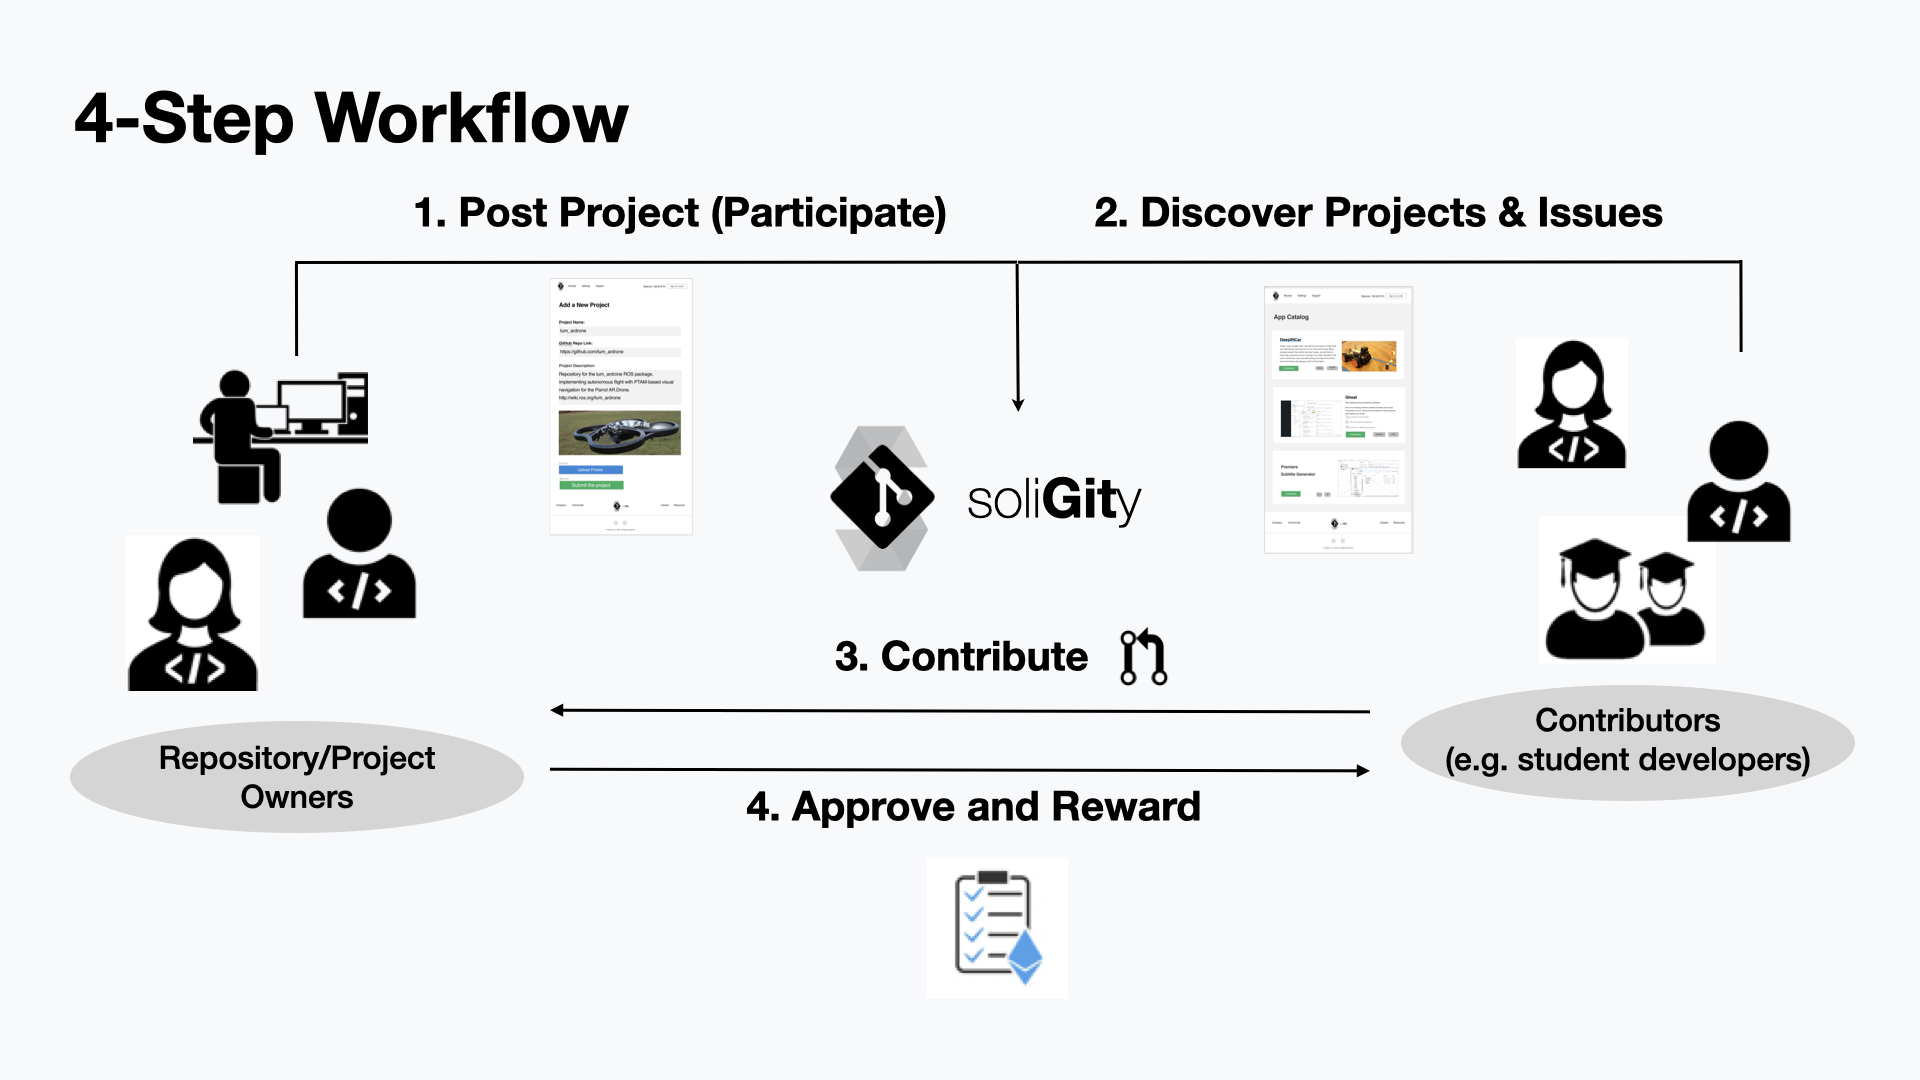
\includegraphics[width=16.5cm]{graphs/00a. workflow.jpeg}
	\caption{SoliGity 4-Step Workflow}
	\label{fig:workflow1}
\end{figure}


\subsection*{Step 1. Post Project}

As mentioned earlier, the SoliGity account is associated with the user’s GitHub account. Once configured, the user can access the list of their own repositories (Figure~\ref{fig:workflow2}a). To have one of their repositories being discovered by everyone on the platform, the project owner must link/add this repo to the project catalog (Figure~\ref{fig:workflow2}b). For every project in the catalog, any user can create issues (Figure~\ref{fig:workflow2}c). All issues created within SoliGity will be book-kept in the SoliGity blockchain DApp, and they will be propagated to GitHub as regular GitHub issues using GitHub APIs. While creating an issue, SoliGity also prompts the user for a price - the amount of cryptocurrency that the project owner will award to the developer when the work is approved. Each issue also comes with a status tracked by the DApp - \textit{Accepting Contributions}, \textit{Pending Approval}, and \textit{Done}. In this stage, a newly-opened issue is in \textit{Accepting Contribution} status.


\begin{figure}[H]
	\centering
	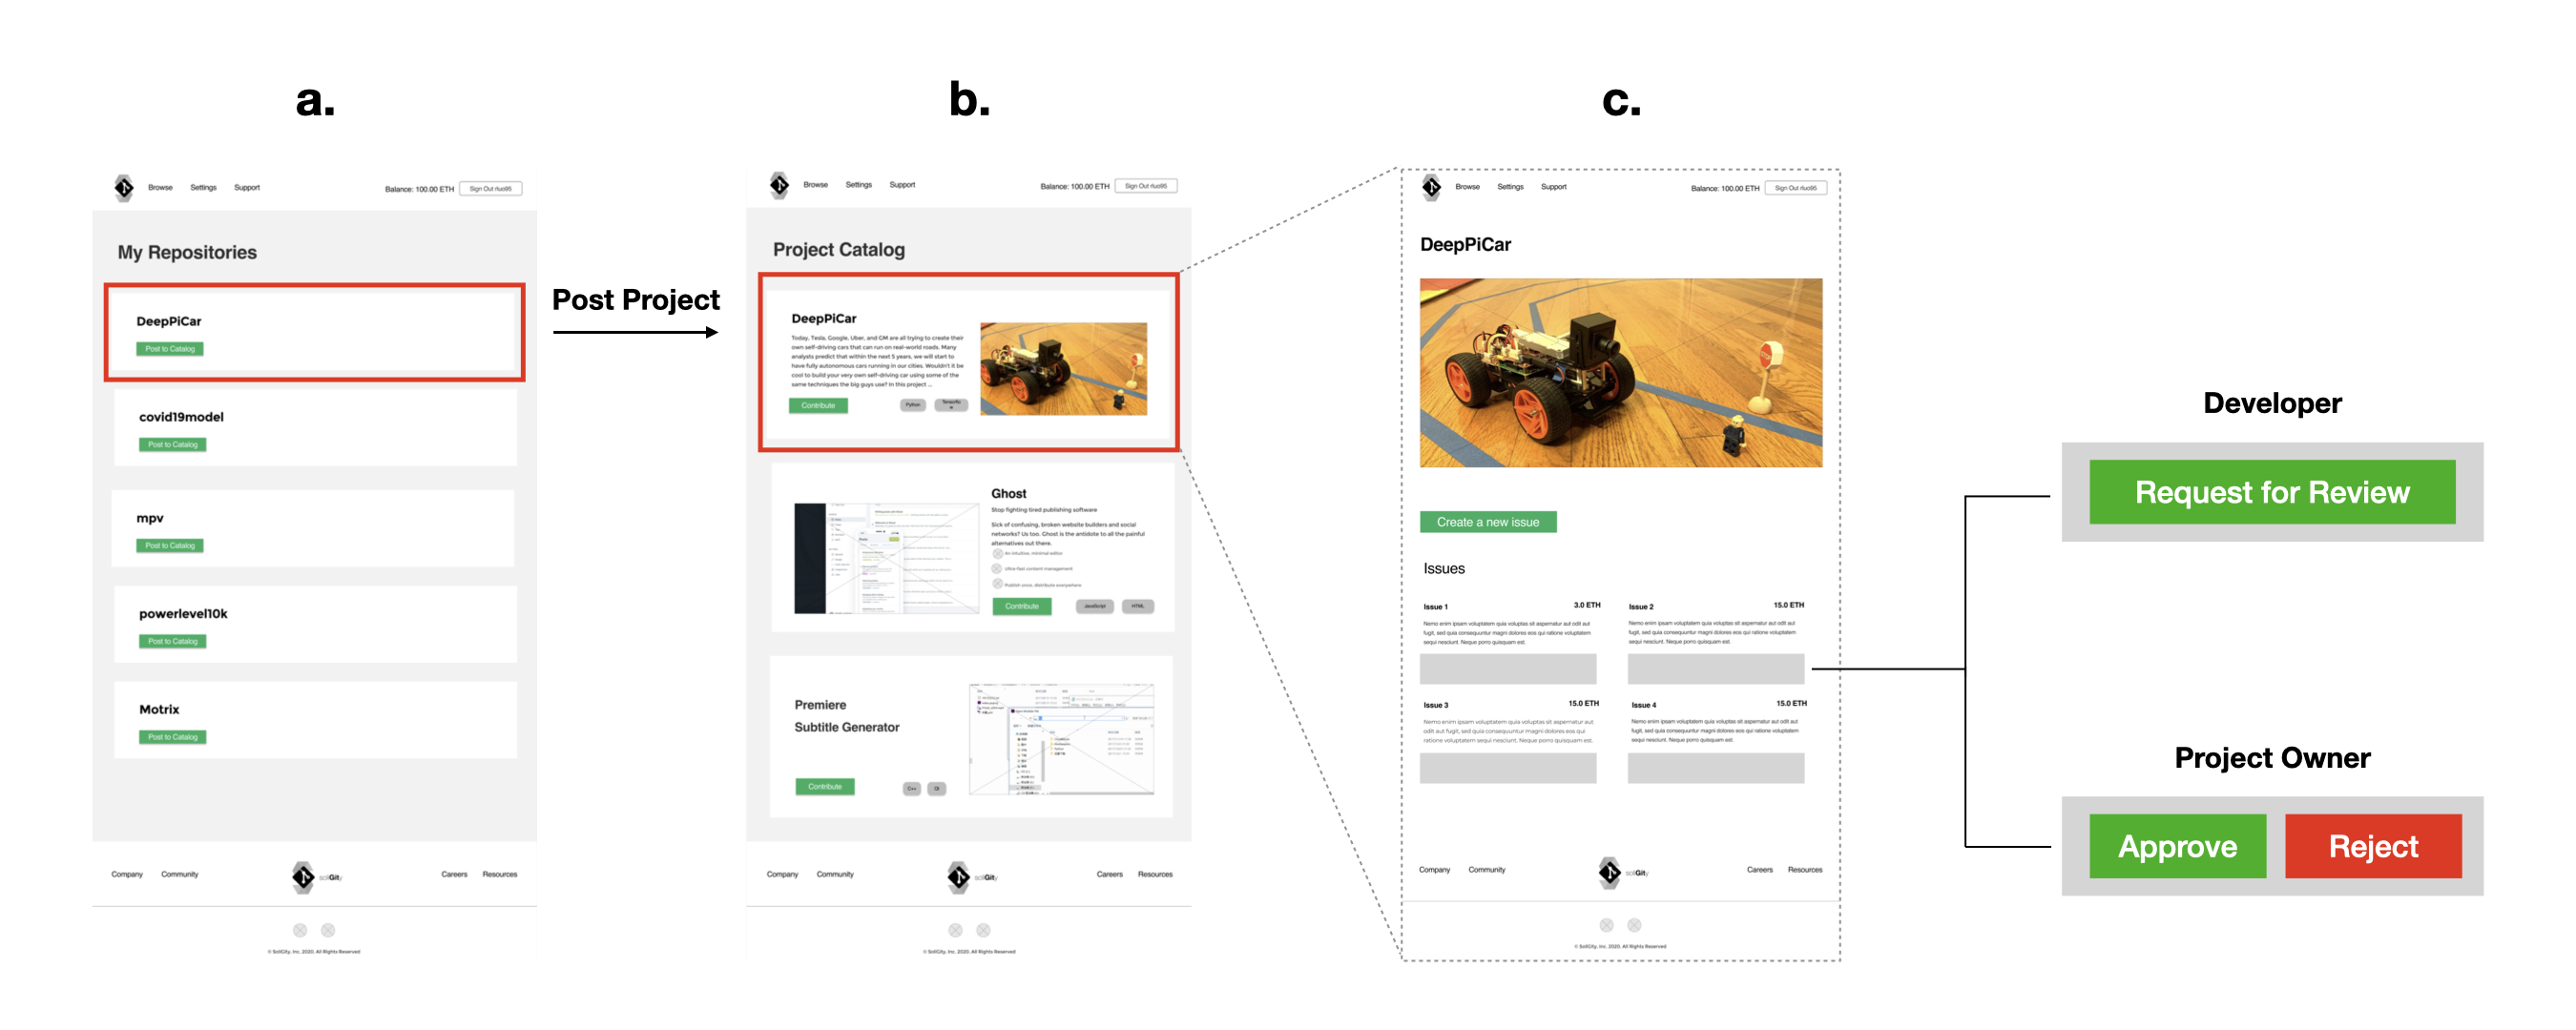
\includegraphics[width=16.5cm]{graphs/00b. workflow.jpeg}
	\caption{SoliGity 4-Step Workflow}
	\label{fig:workflow2}
\end{figure}

\subsection*{Step 2. Discover Project}

Once the projects are posted on the catalog, everyone can discover them. We envision an interface that looks like an App Store, displaying project information in rich details such as project name, pictures, languages \& frameworks etc. The intuitive, friendly experience will be of great benefit for these entry-level developers and students to quickly become interested in a project. The project description page (Figure~\ref{fig:workflow2}c) displays the issues. Note that issues are not limited to bugs - they can also be new features and feasibility studies that’s available for anyone to pick up and make contributions.

\subsection*{Step 3. Making Contribution}

Once the developer finds an issue to work on, he/she must fork the repository to their own GitHub account. We provide a button shortcut to help the developer fork the repo without leaving SoliGity. Then, the development process is identical to regular Git workflow - the developer commits and pushes the work to their forked repo, then makes a pull request when the work is done (Figure~\ref{fig:workflow2}c). Note that the review request is made in SoliGity - this makes sure that both our DApp and GitHub are aware of this activity. On SoliGity, the issue status will be changed to \textit{Pending Approval} from \textit{Accepting Contribution}; on GitHub, a pull request will be made for the project owner to review the code changes.

\subsection*{Step 4. Rewarding Contribution}
When a review request is made, the project owner reviews the code changes on GitHub website as he/she normally does in the traditional Git workflow. If the work is acceptable, the owner will approve the code change on SoliGity by pressing the Approve button (Figure~\ref{fig:workflow2}c). Doing so will (i) Merge the changes to the owner’s Git repository,
(ii) Transfer the bounty in ETH to developer’s wallet,
(iii) Change the issue status from \textit{Pending Approval} to \textit{Done}. In case the owner is not satisfied with the code changes, he/she can reject the contribution by pressing the Reject button (Figure X~\ref{fig:workflow2}c). This will set the issue status back to Accepting Contribution and the process can be re-started.  \\


\noindent Since the GitHub commands including Issue Creation, Fork, and Making Pull Request are fully integrated into SoliGity, the entire workflow is intuitive and straightforward. The transaction takes place between the project owner and the developer nearly instantly, securely without third parties. All of these functional and non-functional features make SoliGity redefine the open-source project rewarding mechanism. In the next section we demonstrate our working prototype step-by-step.

\section{Step-by-step Screenshot with Explanation}
In this section, we demonstrate SoliGity step-by-step. 


\subsection*{Step 0. Initial Setup}
 \begin{enumerate}
   \item DApp Setup
       \begin{figure}[H]
    	\centering
        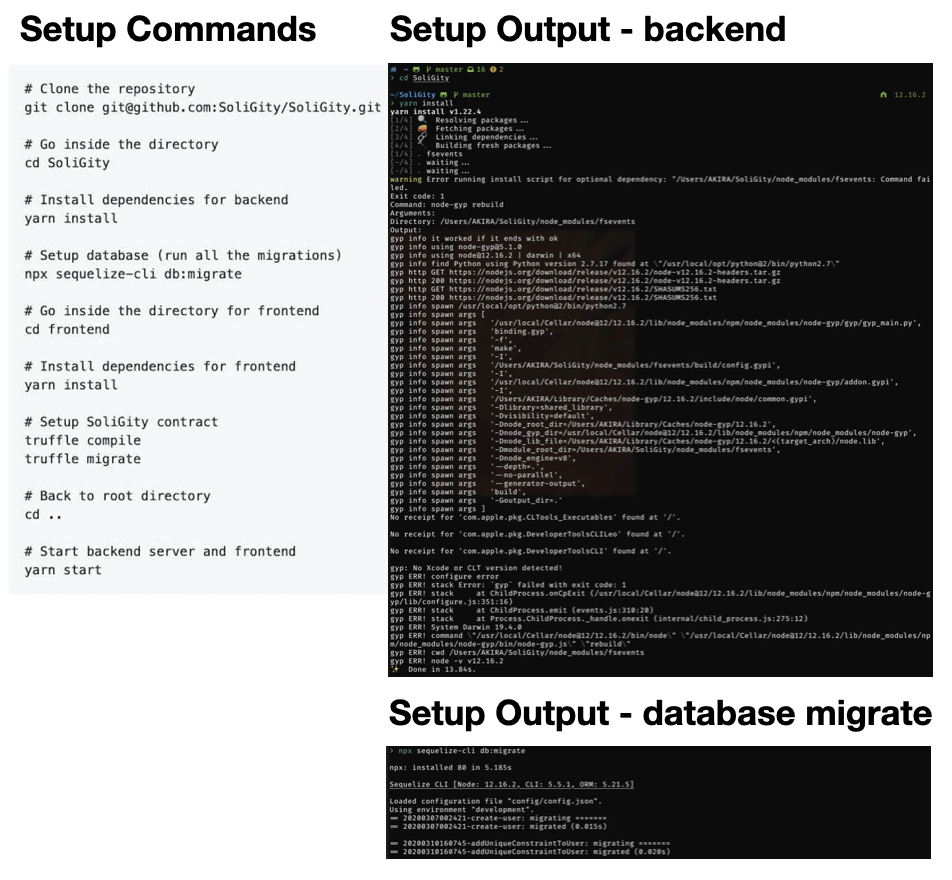
\includegraphics[height=7.5cm]{graphs/46. setup_1.png}\\
    	\caption{SoliGity Setup}
    	\label{fig:setup1}
        \end{figure}
    
        \begin{figure}[H]
        	\centering
            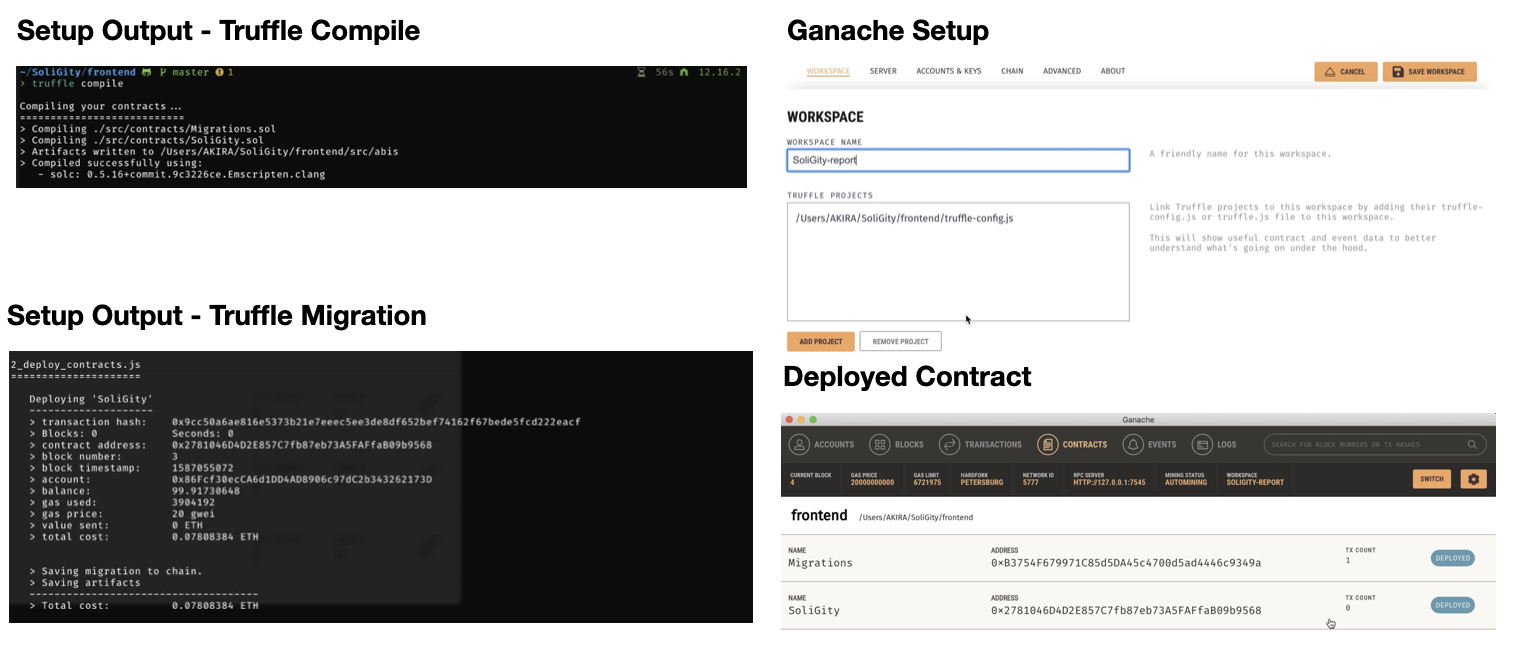
\includegraphics[height=7.5cm]{graphs/47. setup_2.png}\\
        	\caption{SoliGity Setup Cont'd}
        	\label{fig:setup2}
        \end{figure}

        \begin{figure}[H]
        	\centering
            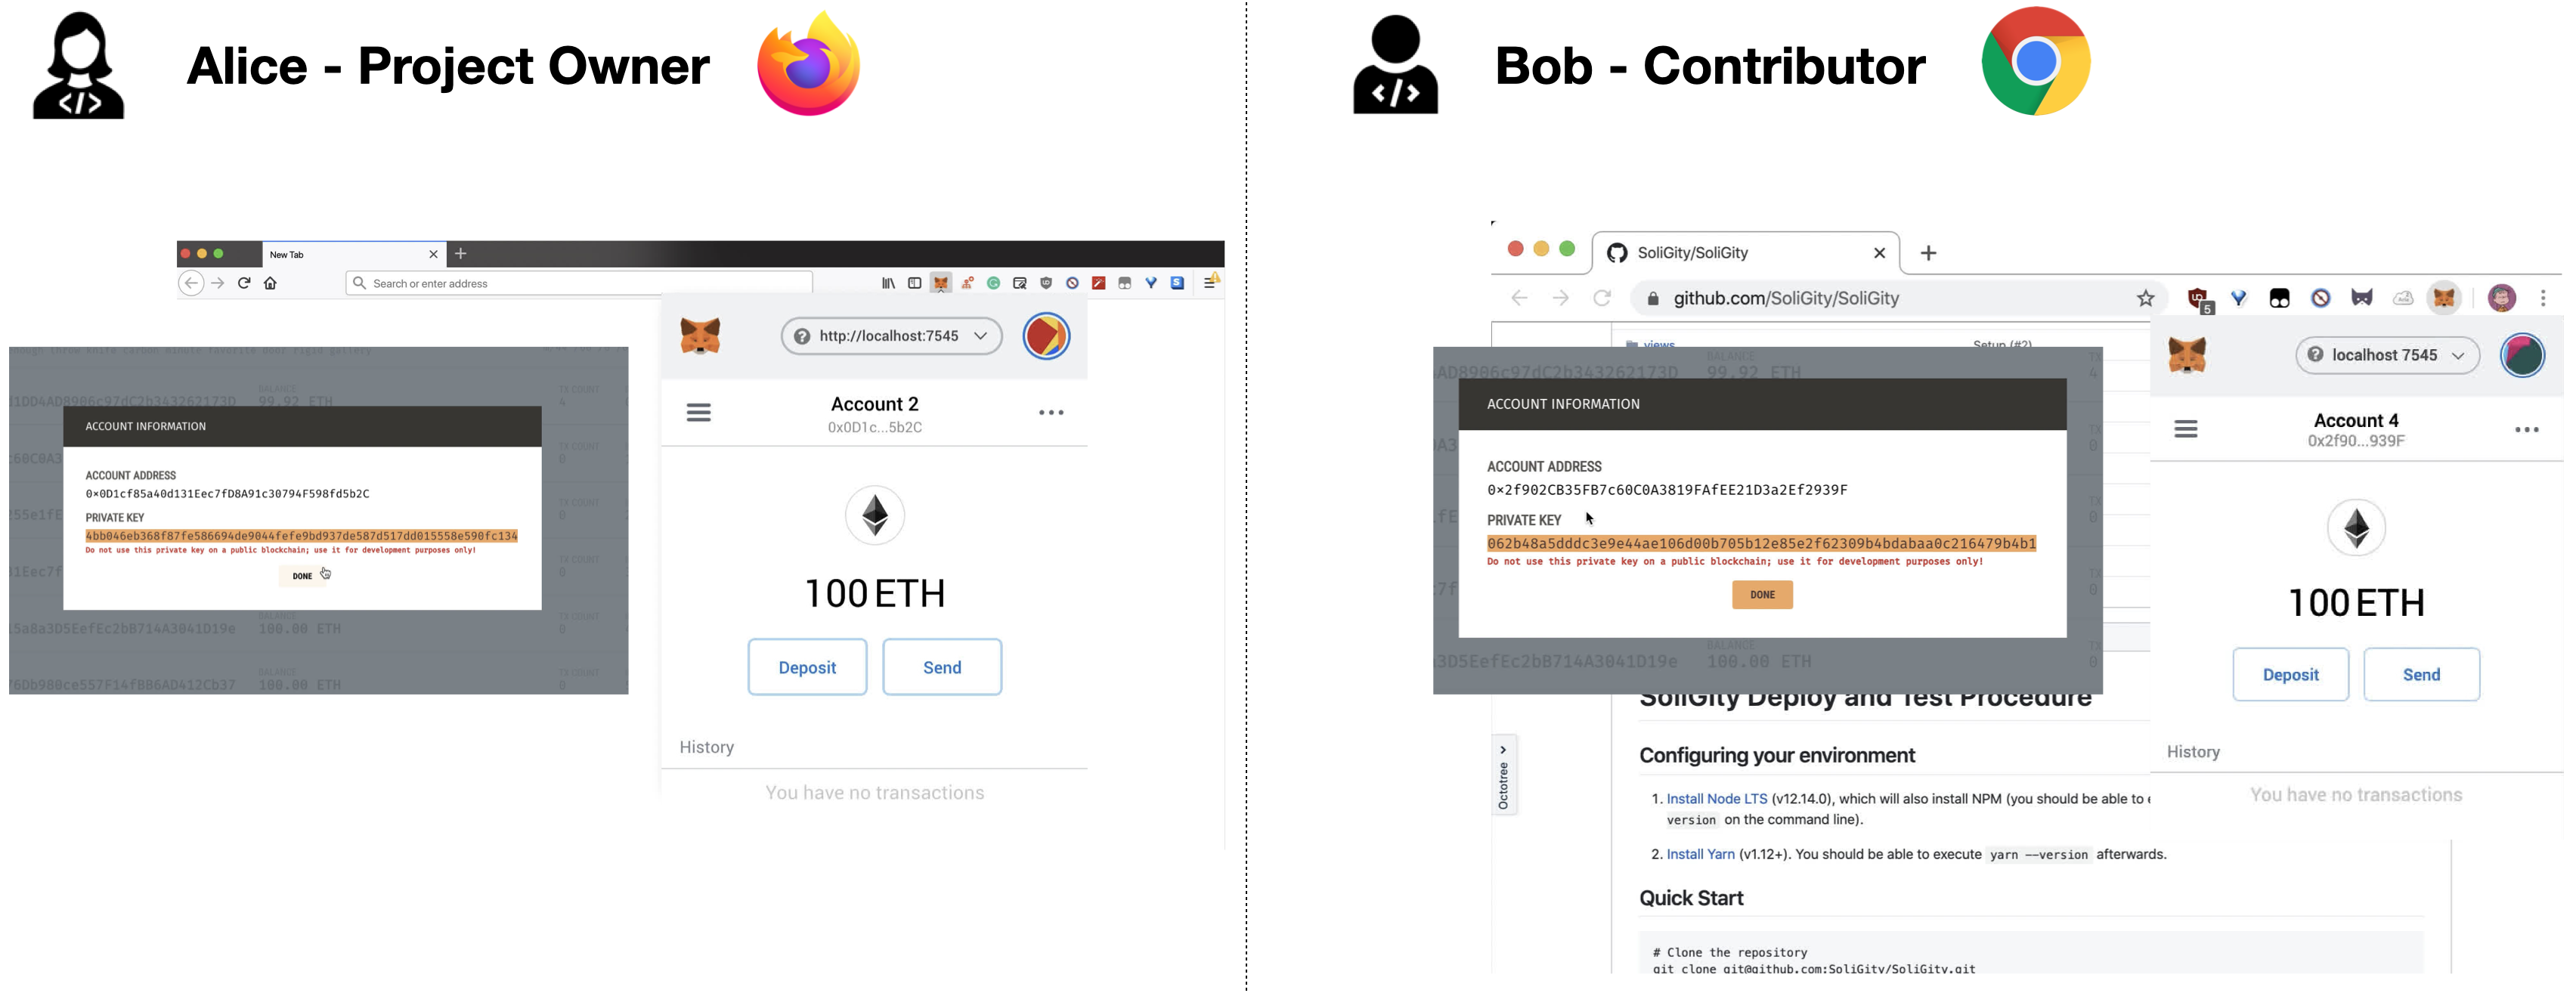
\includegraphics[width=16.5cm]{graphs/48. setup_3.png}\\
        	\caption{SoliGity Setup Cont'd}
        	\label{fig:setup3}
        \end{figure}

   \item SolGity Account Setup
        \begin{figure}[H]
        	\centering
            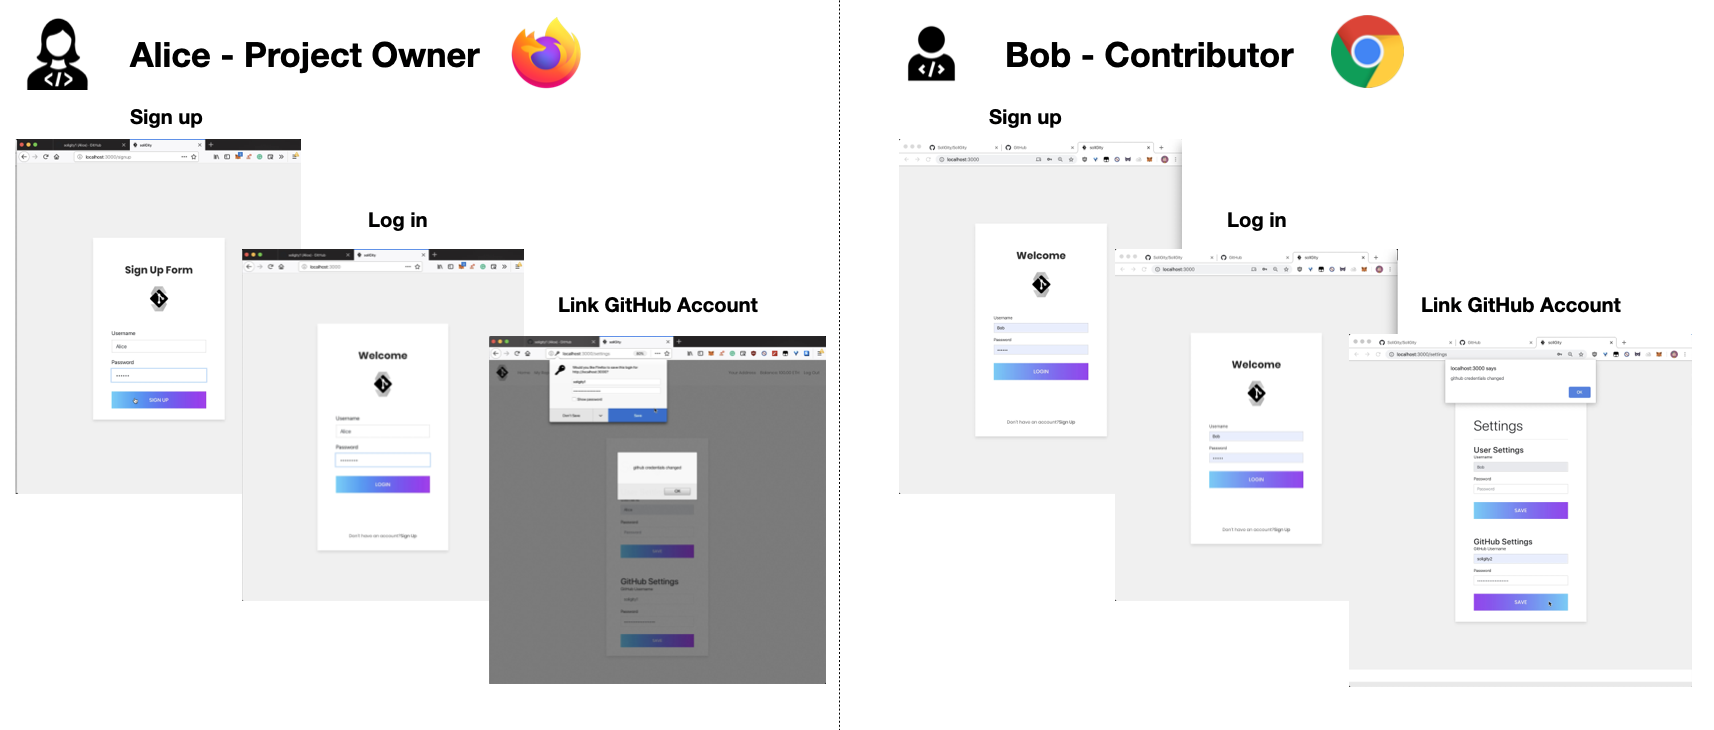
\includegraphics[width=16.5cm]{graphs/49. setup_4.png}\\
        	\caption{SoliGity Setup Cont'd}
        	\label{fig:setup4}
        \end{figure}
 \end{enumerate}

\subsection*{Step 1. Post Project}
 \begin{enumerate}
    \item Post Project to Catalog
         \begin{figure}[H]
        	\centering
            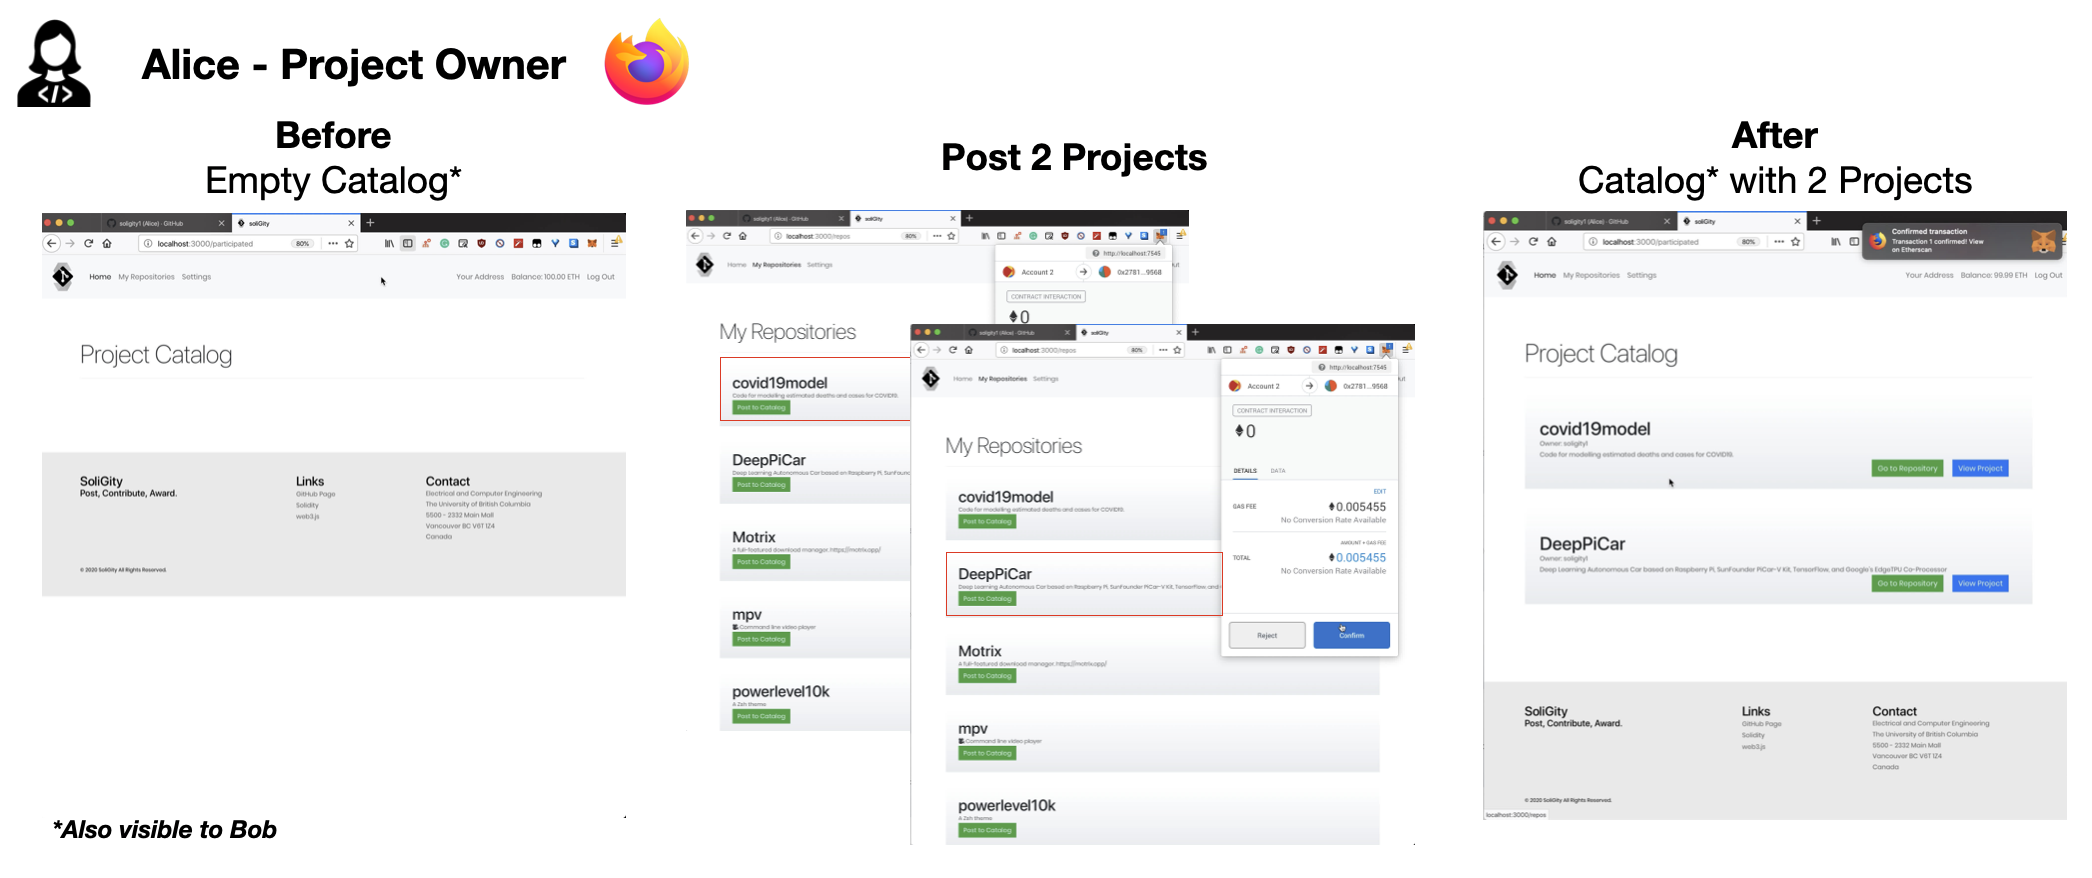
\includegraphics[width=16.5cm]{graphs/50. post_1.png}\\
        	\caption{Project owner posting 2 projects to Project Catalog}
        	\label{fig:post1}
        \end{figure}

    \item Create Issue
    
         \begin{figure}[H]
        	\centering
            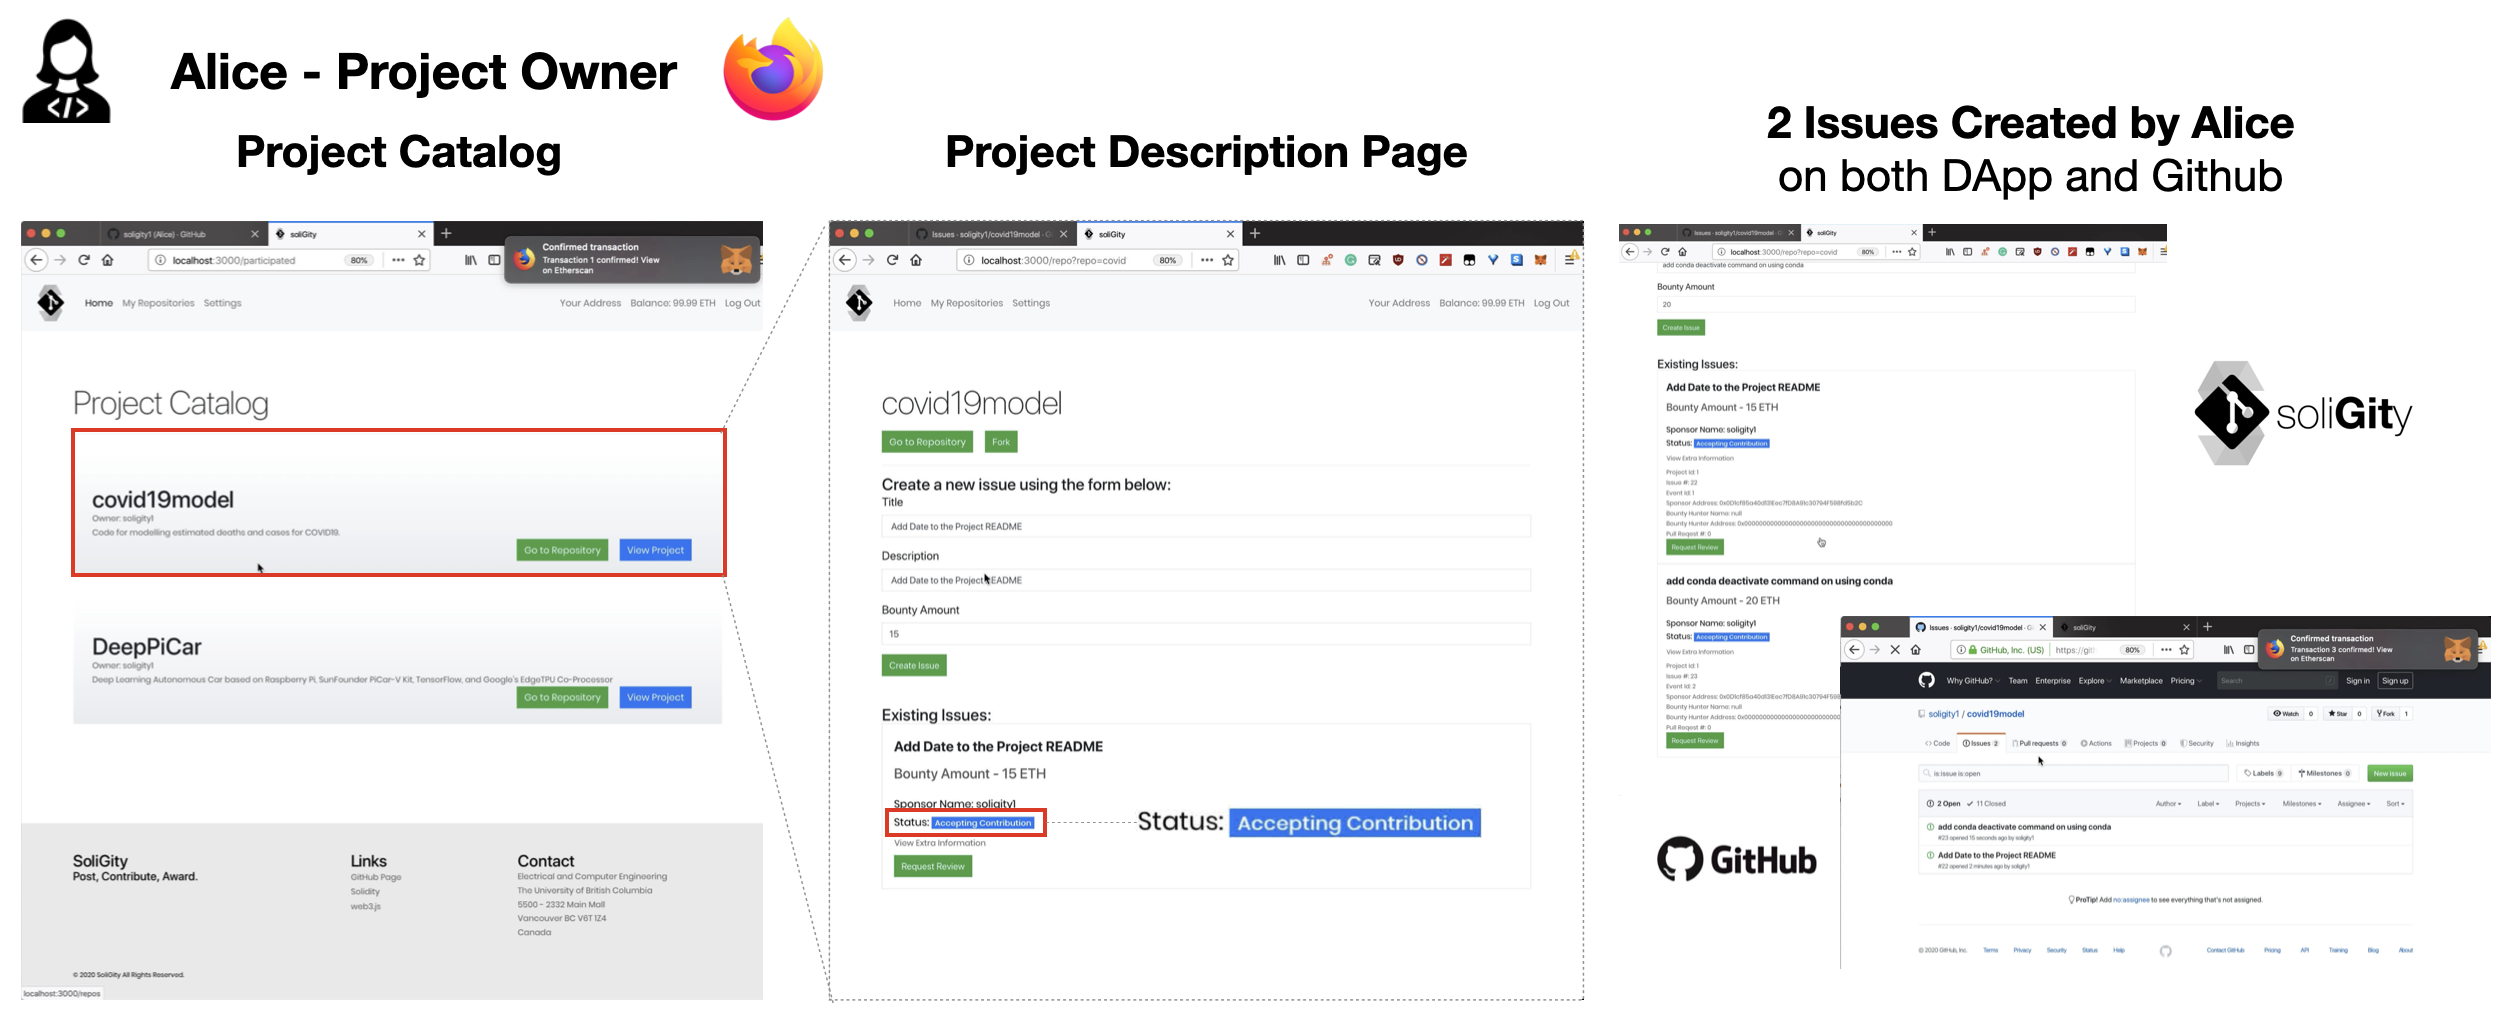
\includegraphics[width=16.5cm]{graphs/51. post_2.png}\\
        	\caption{Project owner creating 2 issues for a project}
        	\label{fig:post2}
        \end{figure}

 \end{enumerate}


\subsection*{Step 2. Discover Project}

     \begin{figure}[H]
    	\centering
        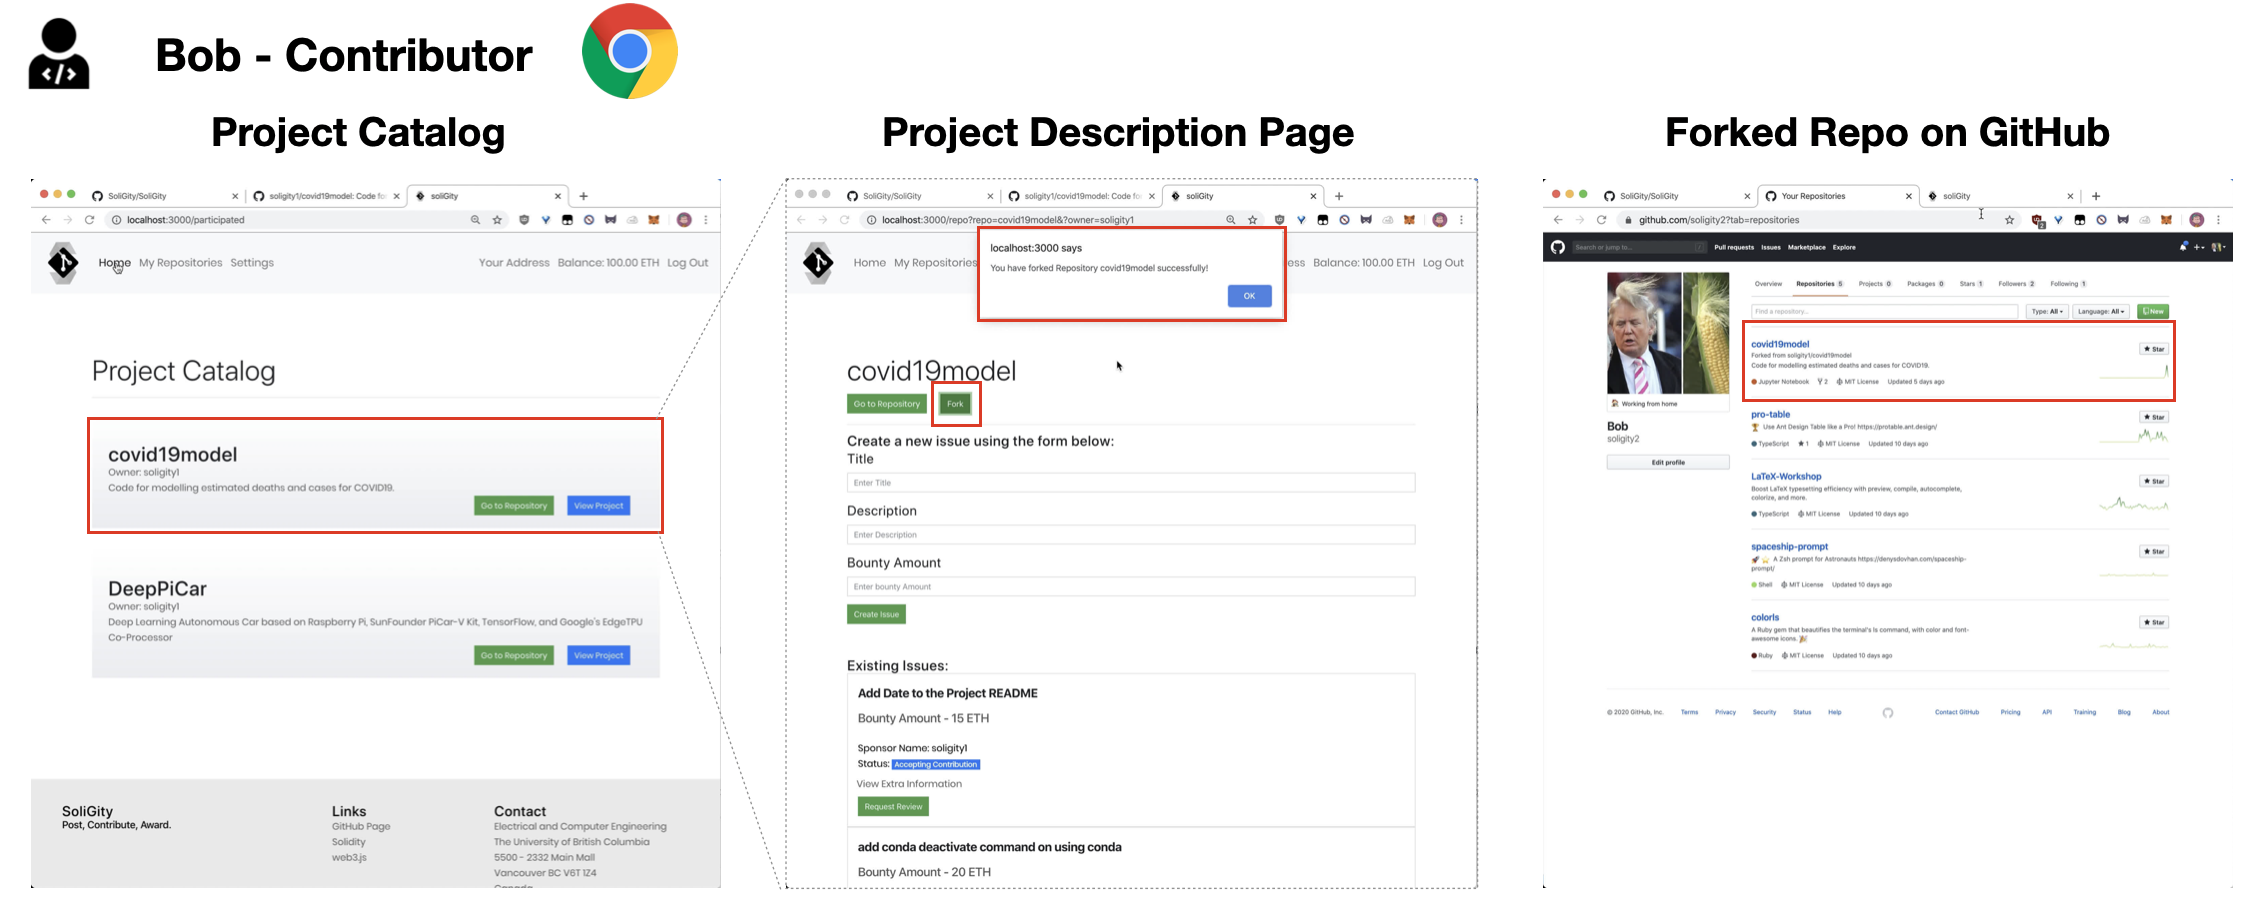
\includegraphics[width=16.5cm]{graphs/52. discover_1.png}\\
    	\caption{Contributor discovering projects and choosing an issue to work on}
    	\label{fig:discover1}
    \end{figure}


\subsection*{Step 3. Making Contribution}


\subsection*{Step 4. Rewarding Contribution}





% 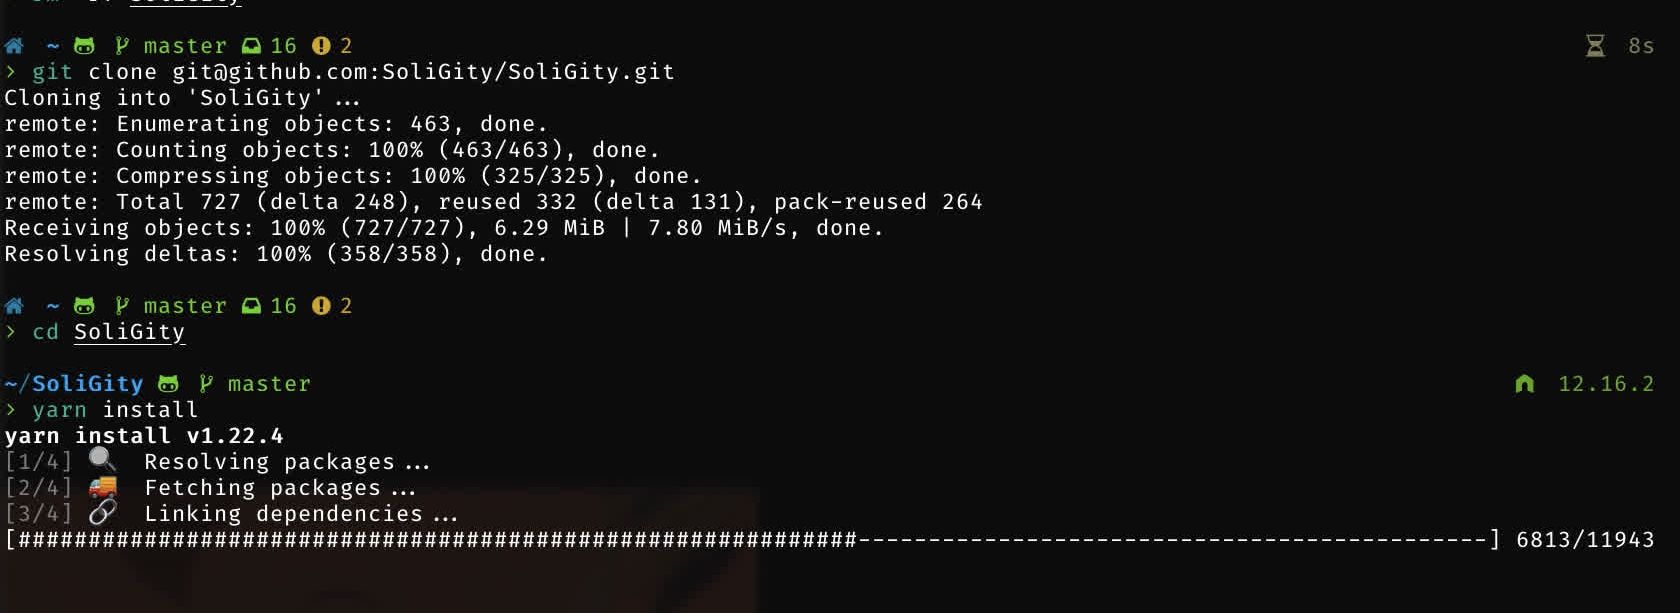
\includegraphics[height=7cm]{graphs/01. git_clone}

% 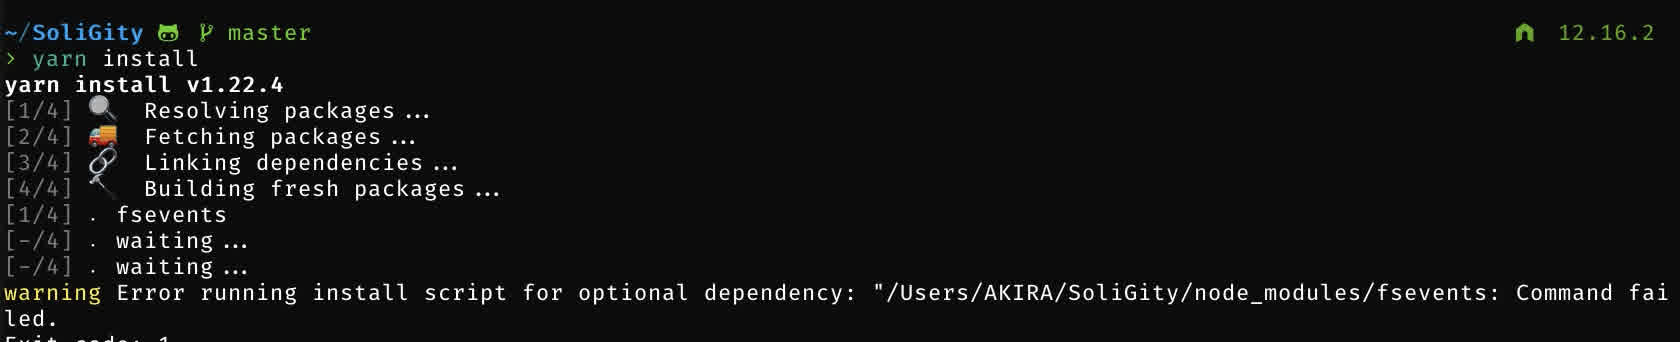
\includegraphics[height=7cm]{graphs/02. yarn_install_backend}

% 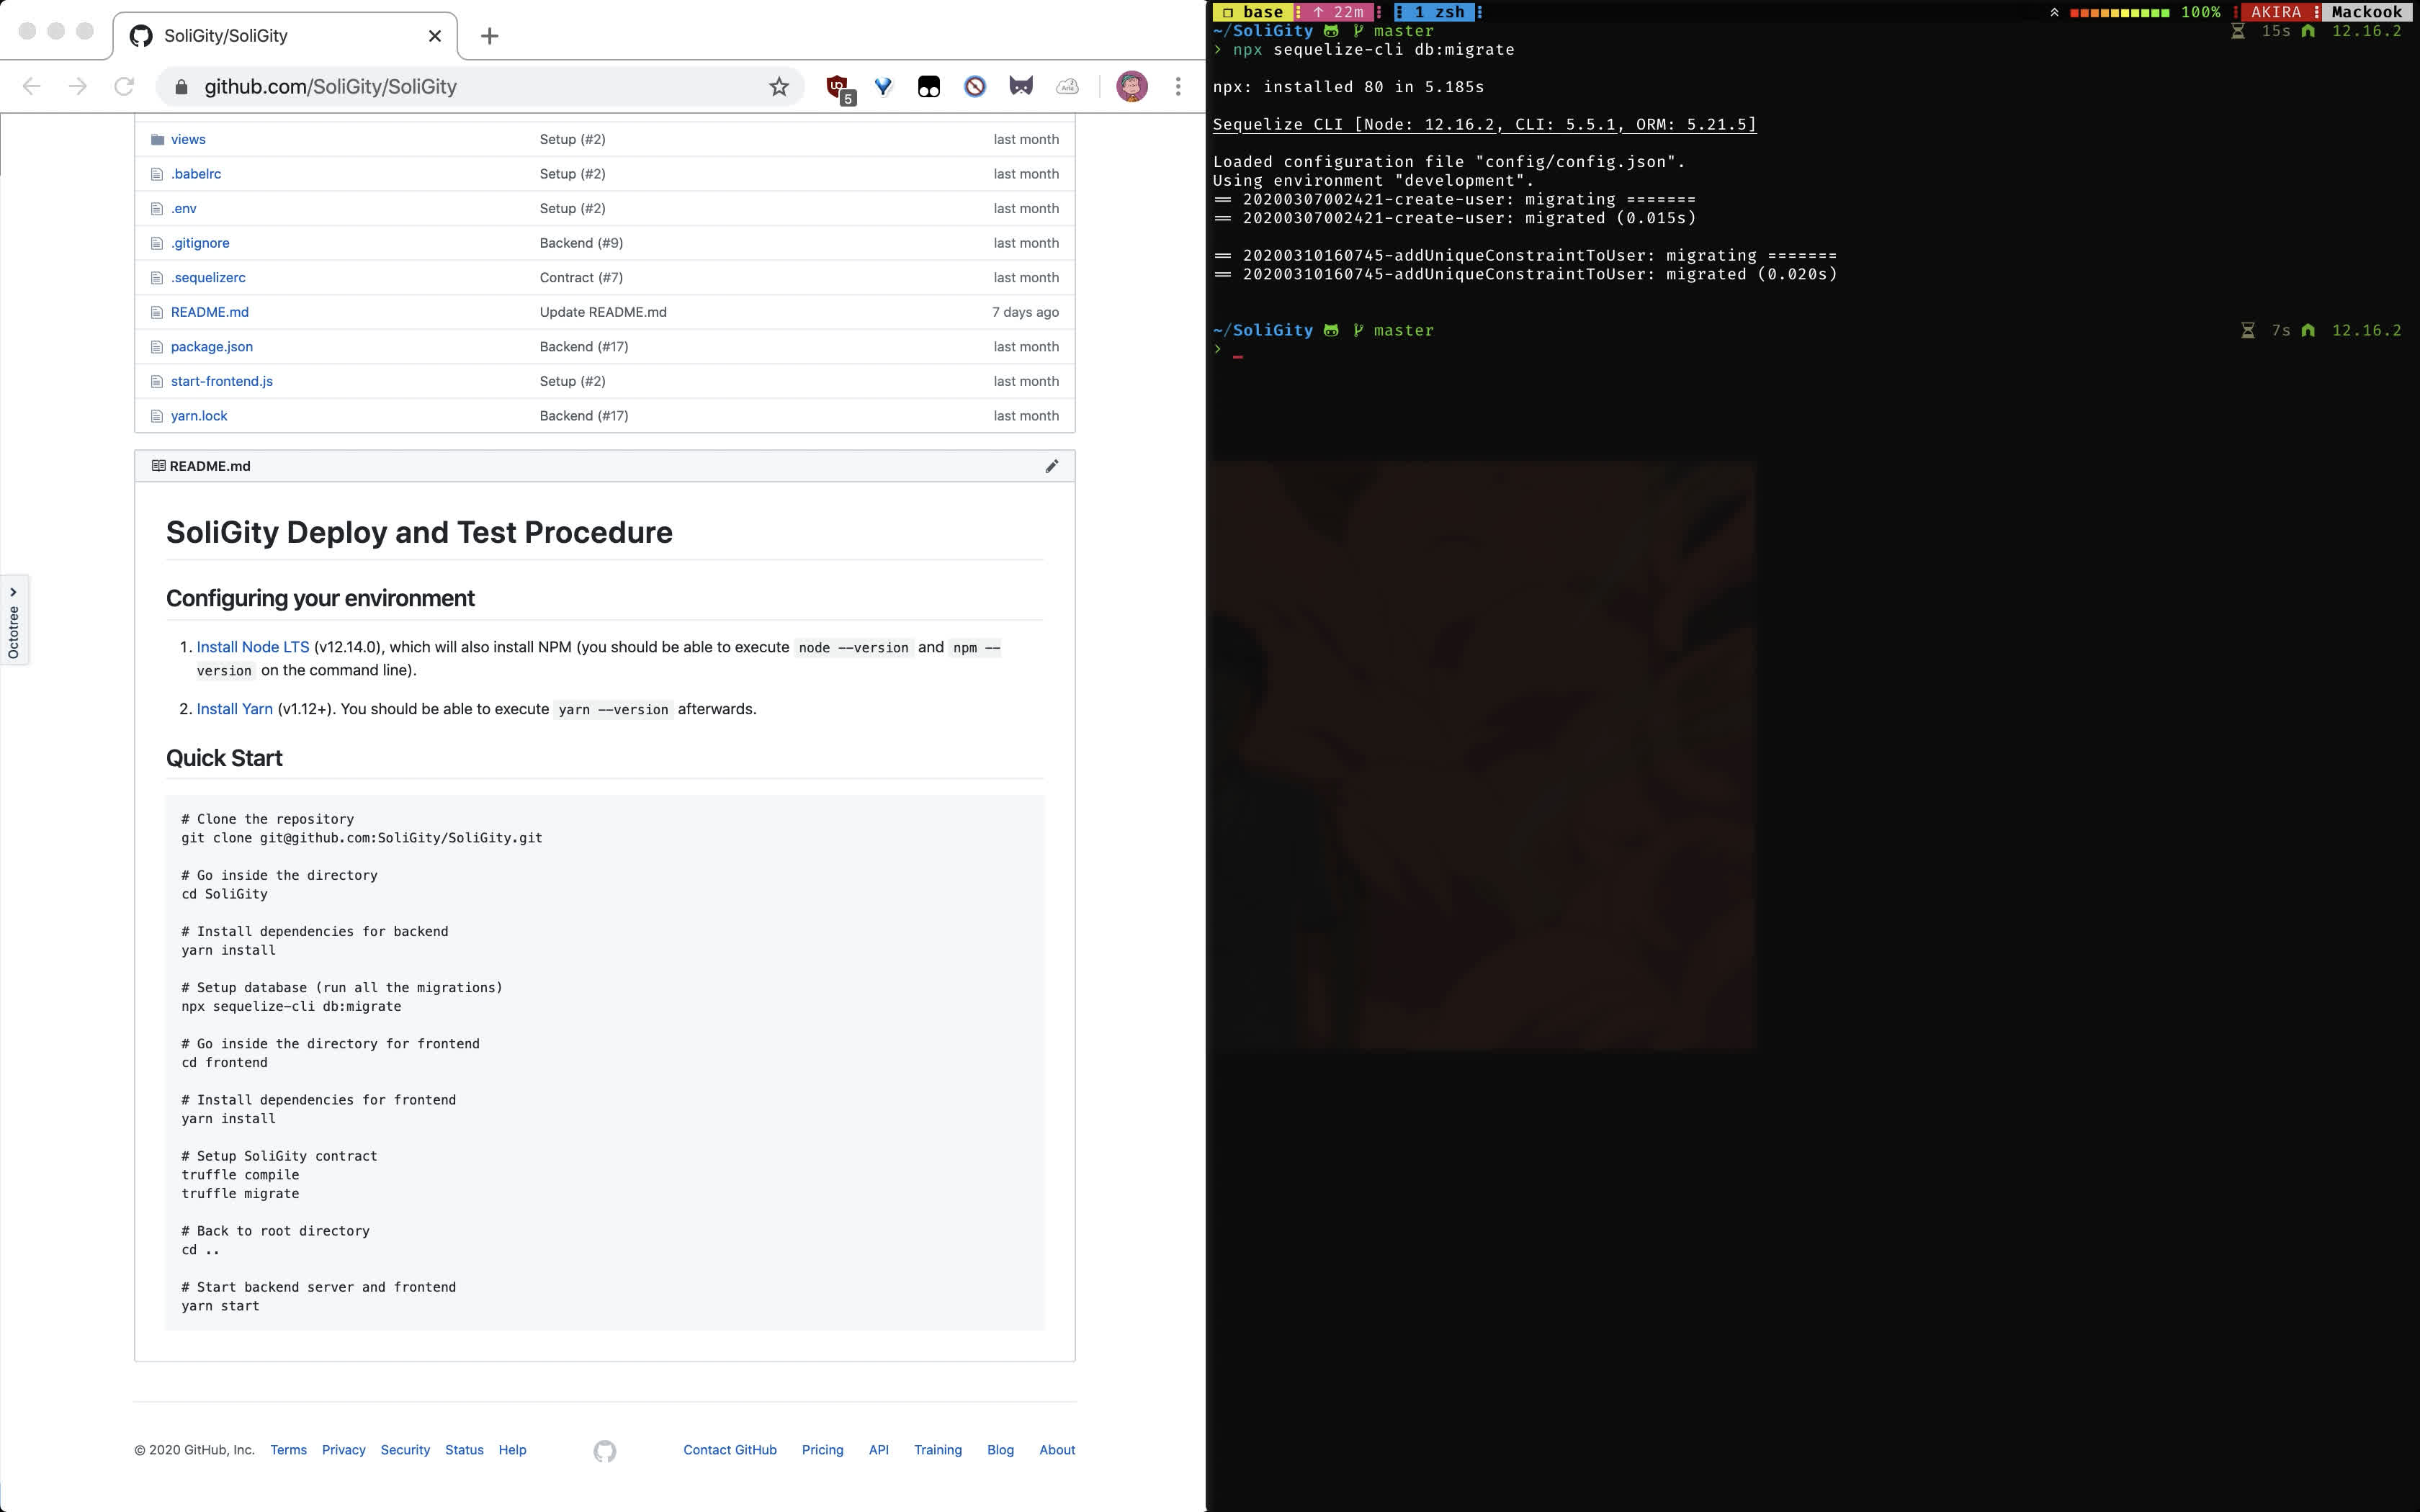
\includegraphics[height=7cm]{graphs/03. user_db_migrate}

% 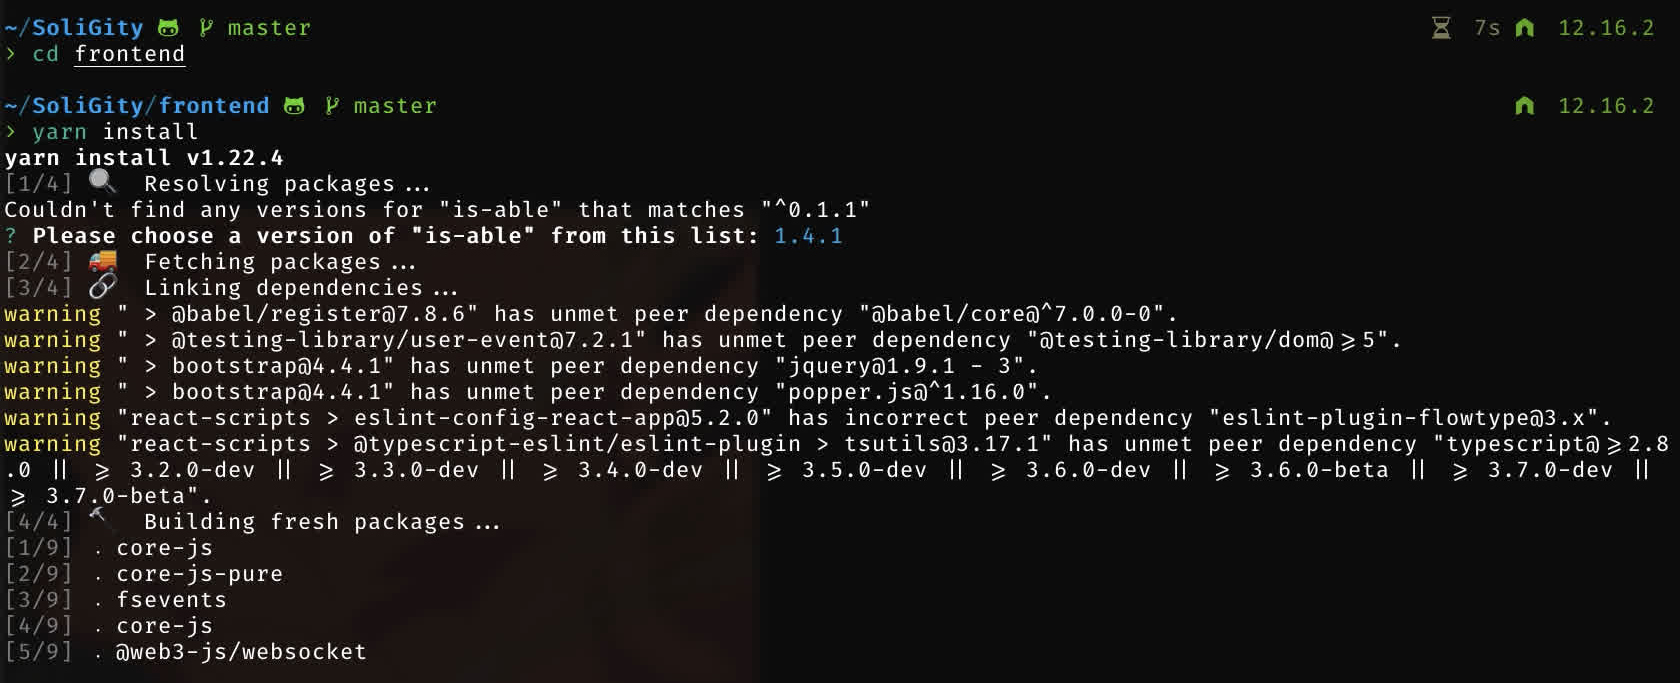
\includegraphics[height=7cm]{graphs/04. yarn_install_frontend}

% 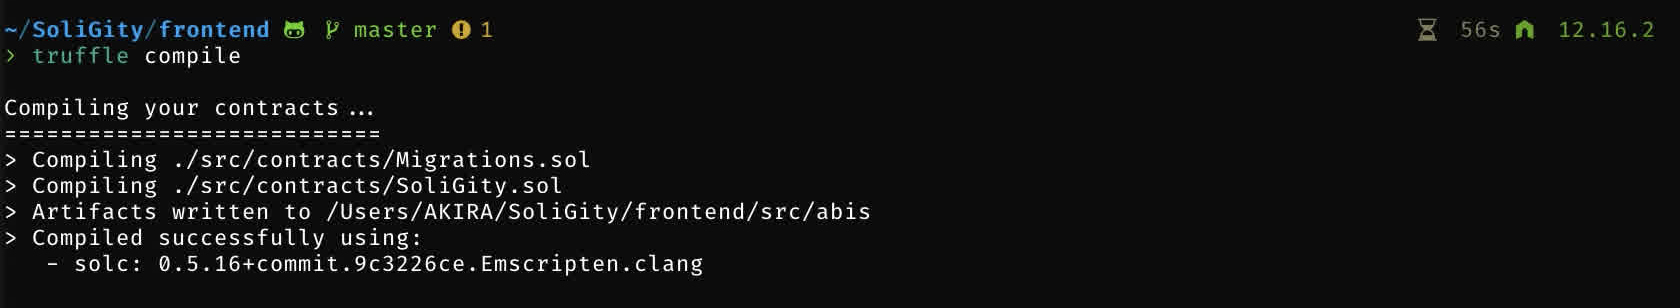
\includegraphics[height=7cm]{graphs/05. truffle_compile}

% 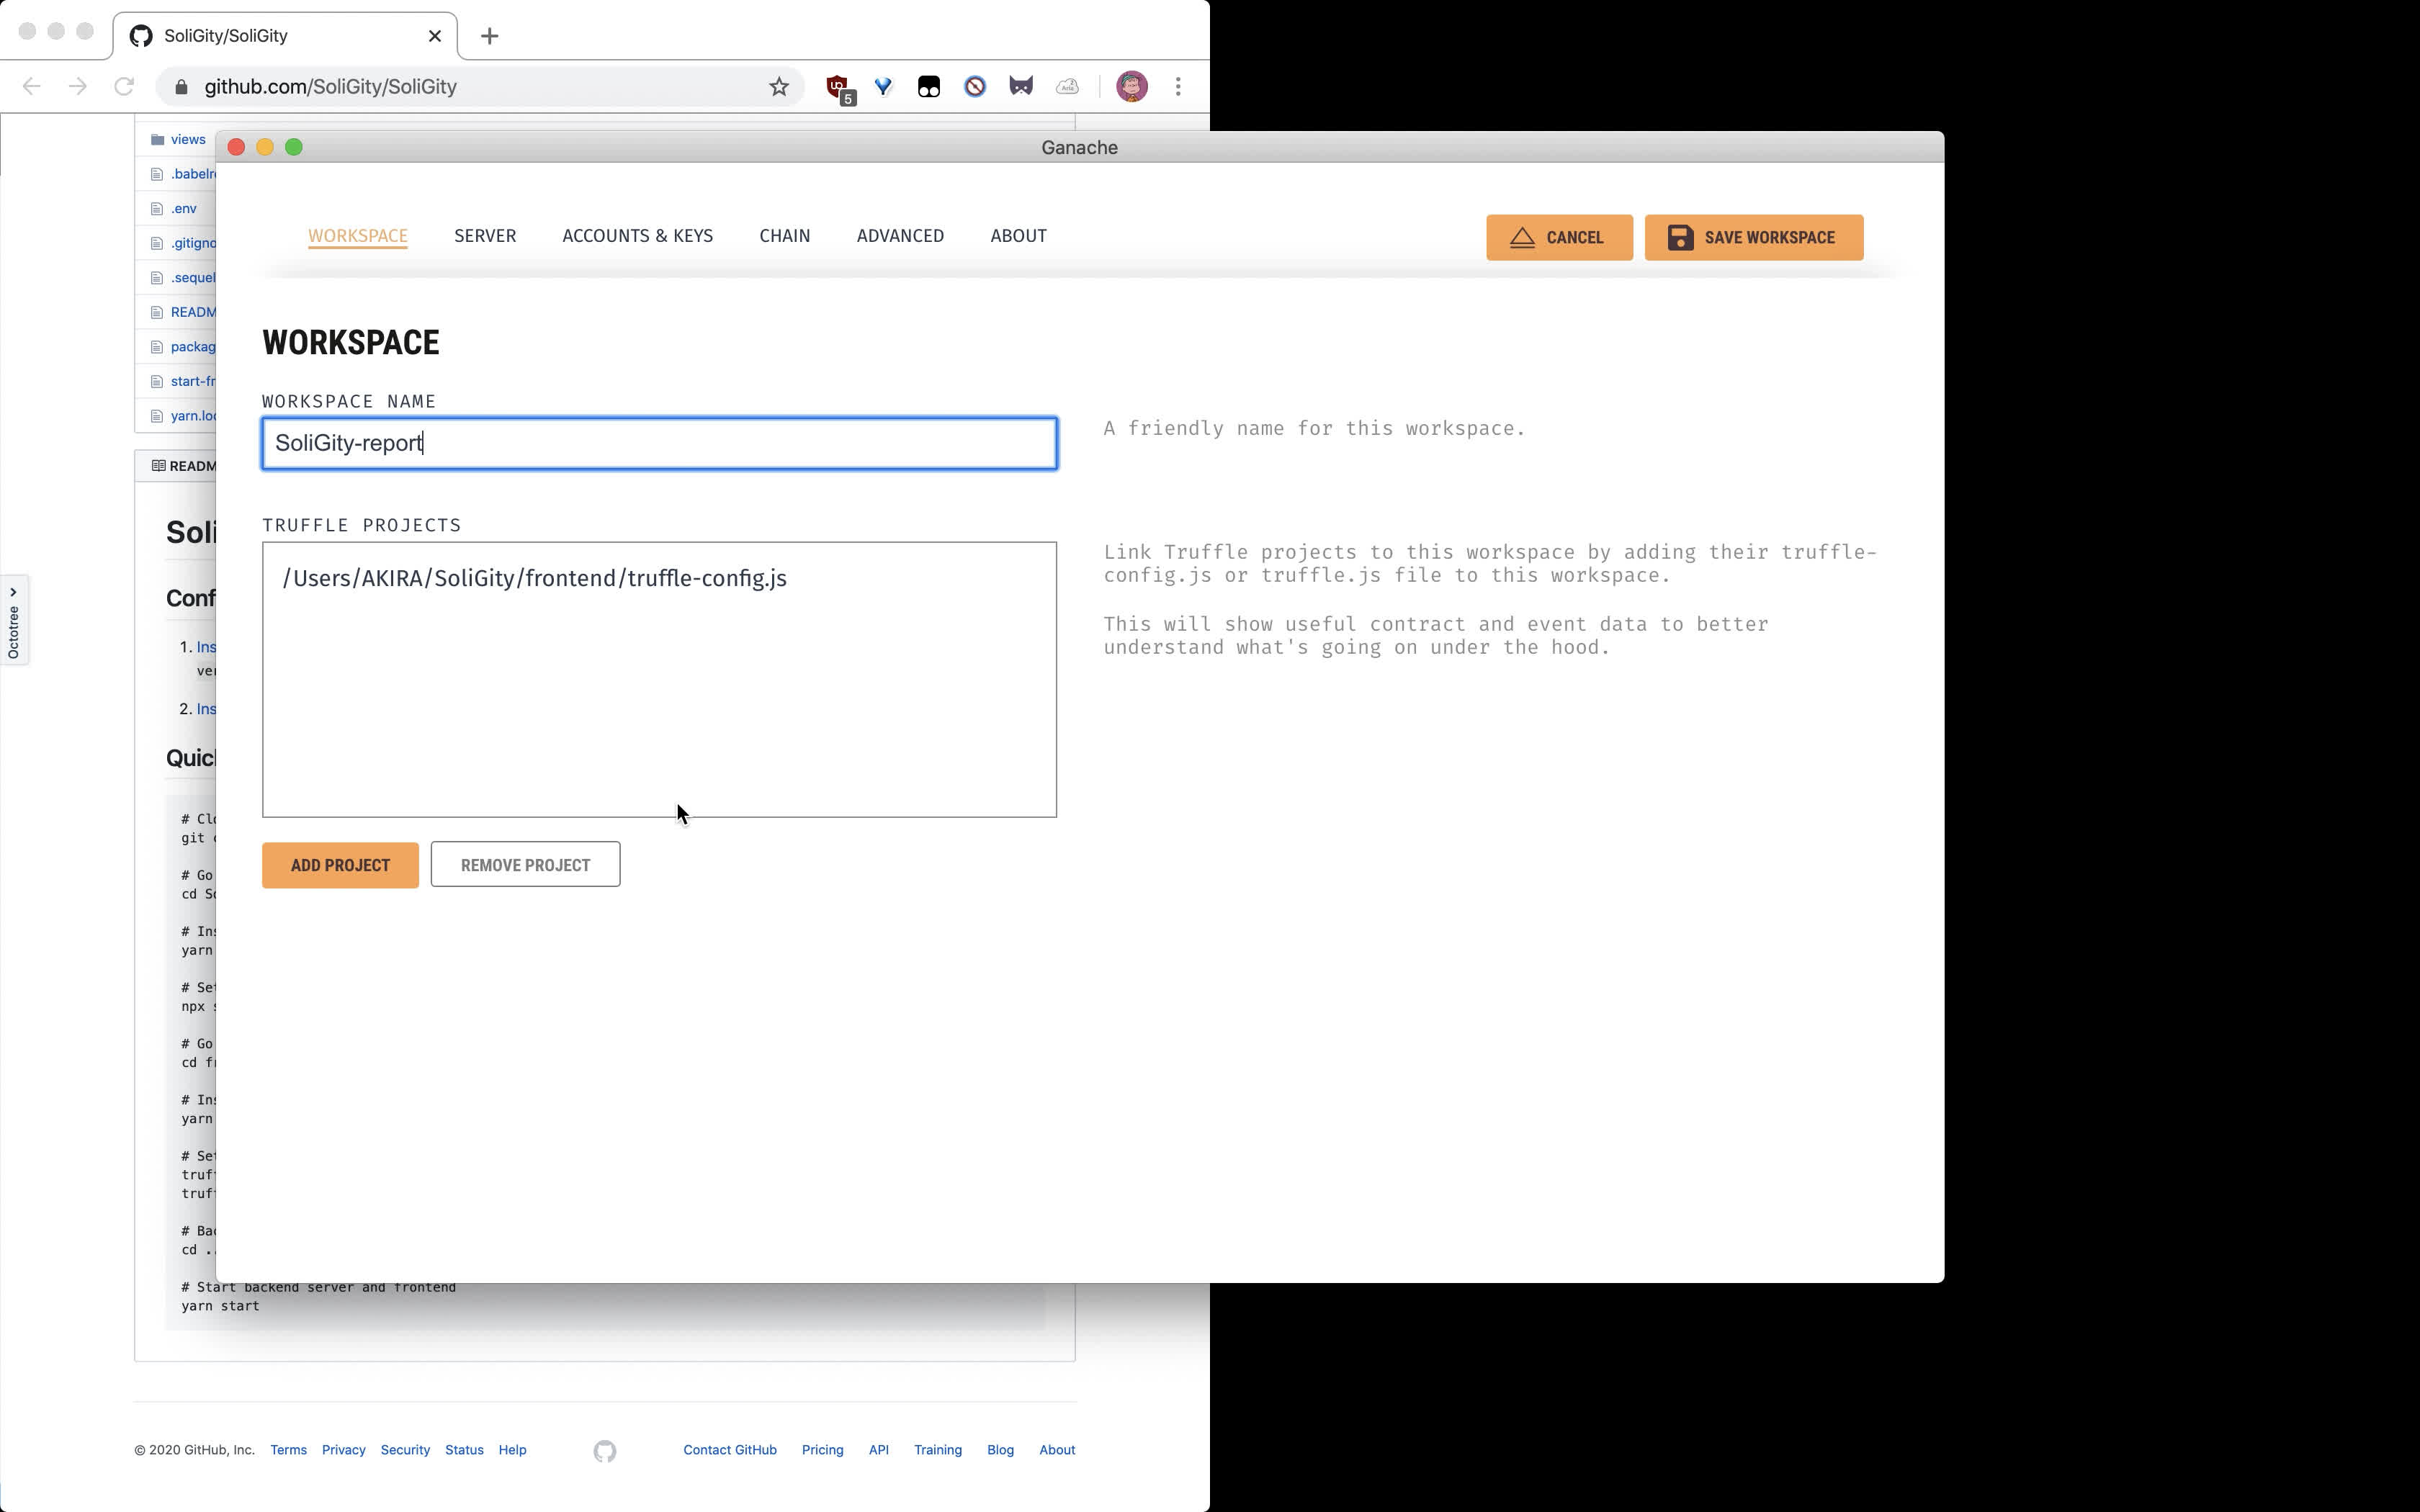
\includegraphics[height=7cm]{graphs/06. ganache_setup}

% 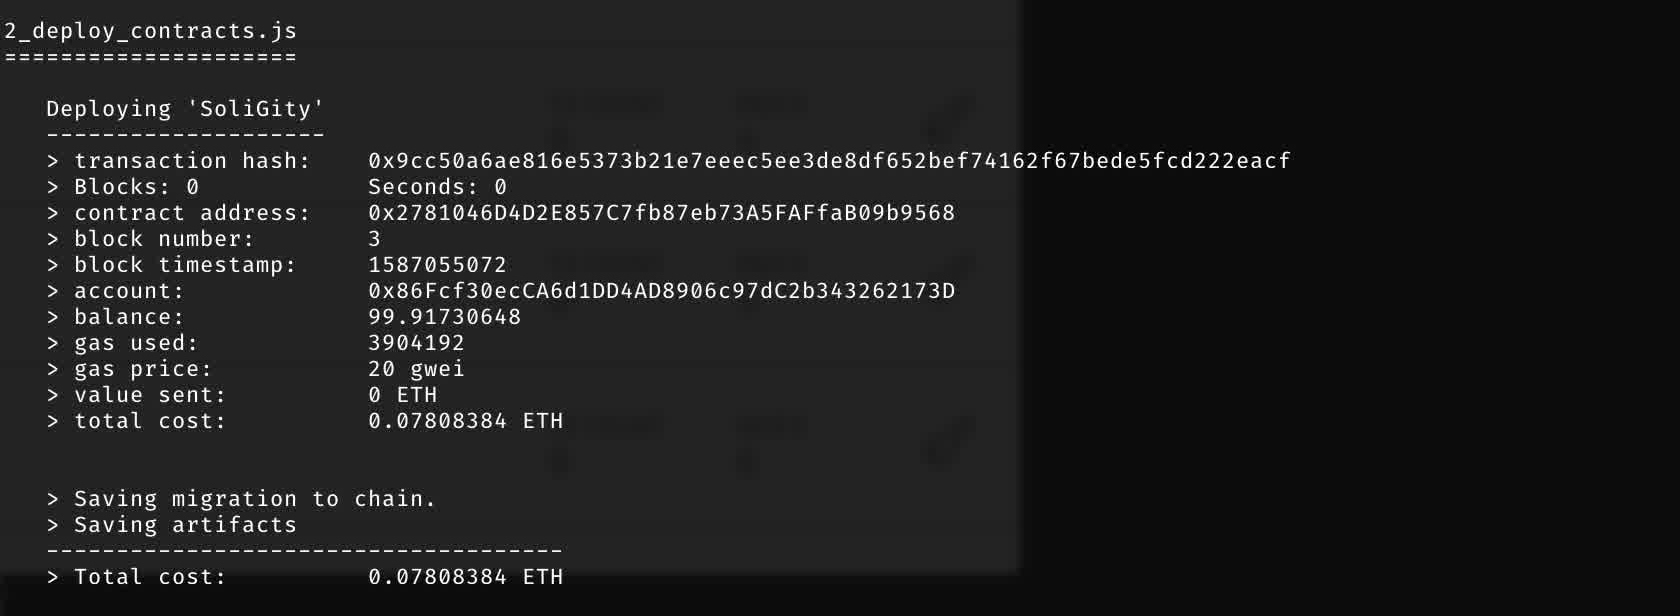
\includegraphics[height=7cm]{graphs/07. truffle_migrate}

% 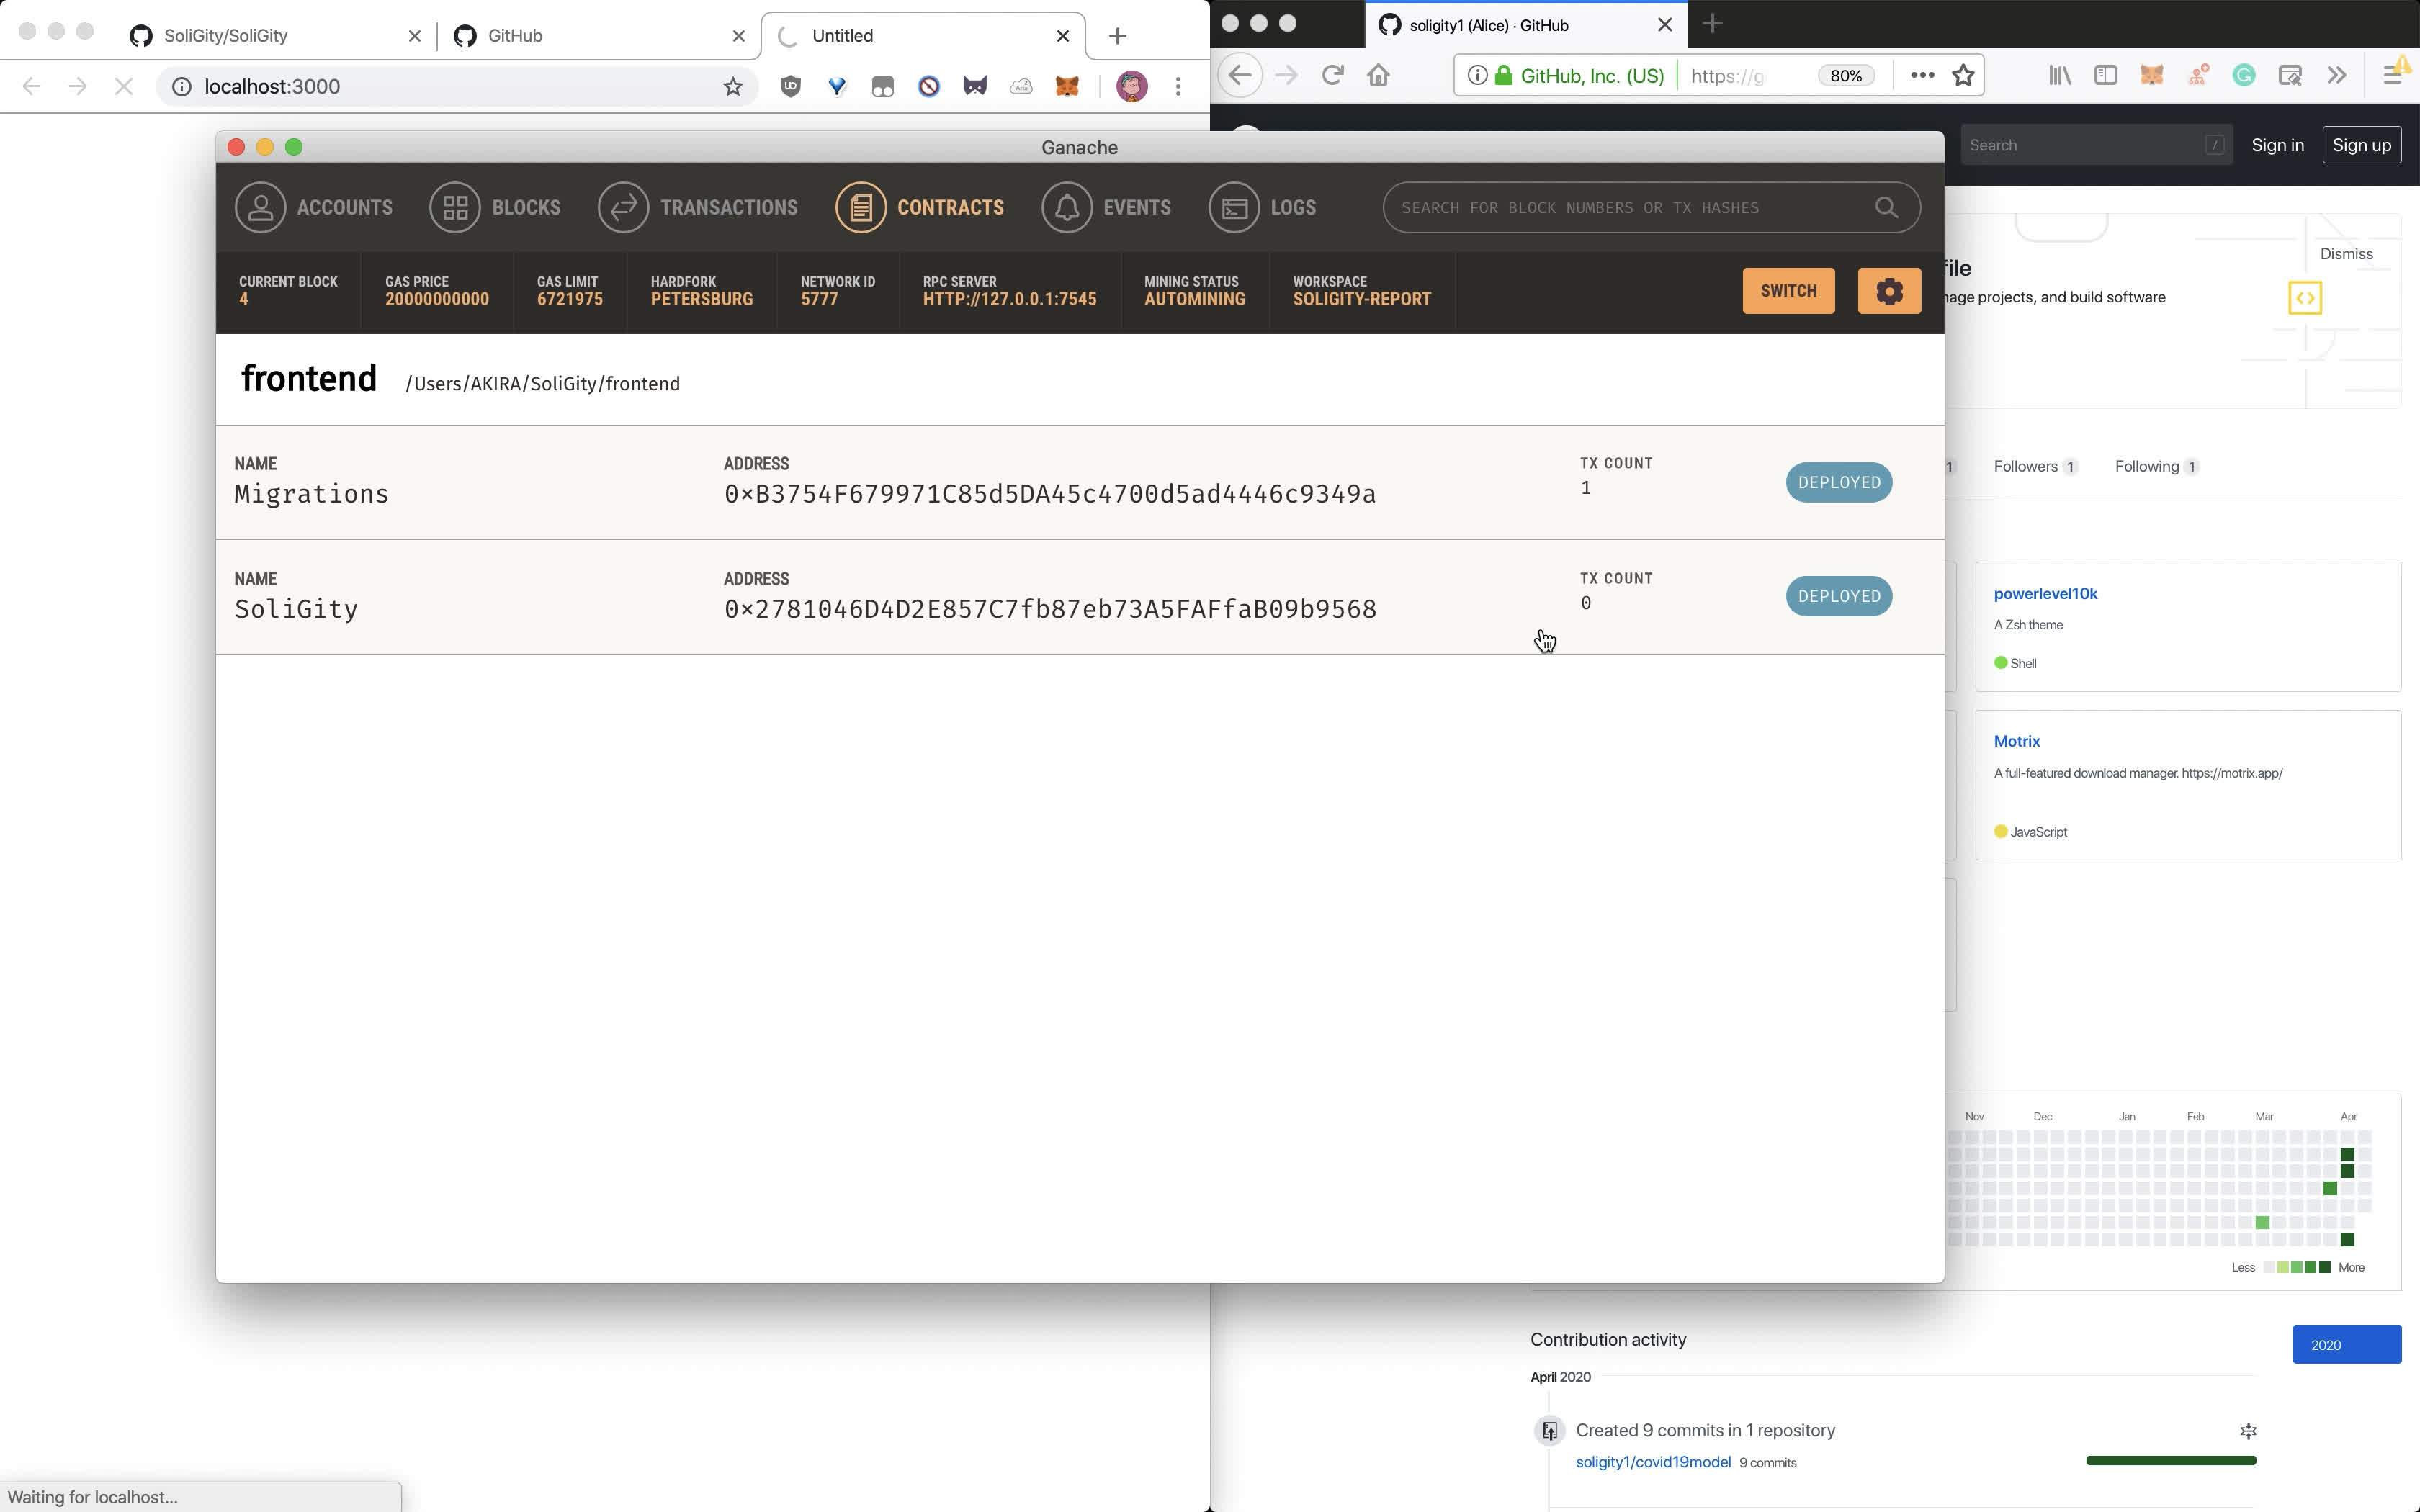
\includegraphics[height=7cm]{graphs/08. ganache_deployed_contract}

% 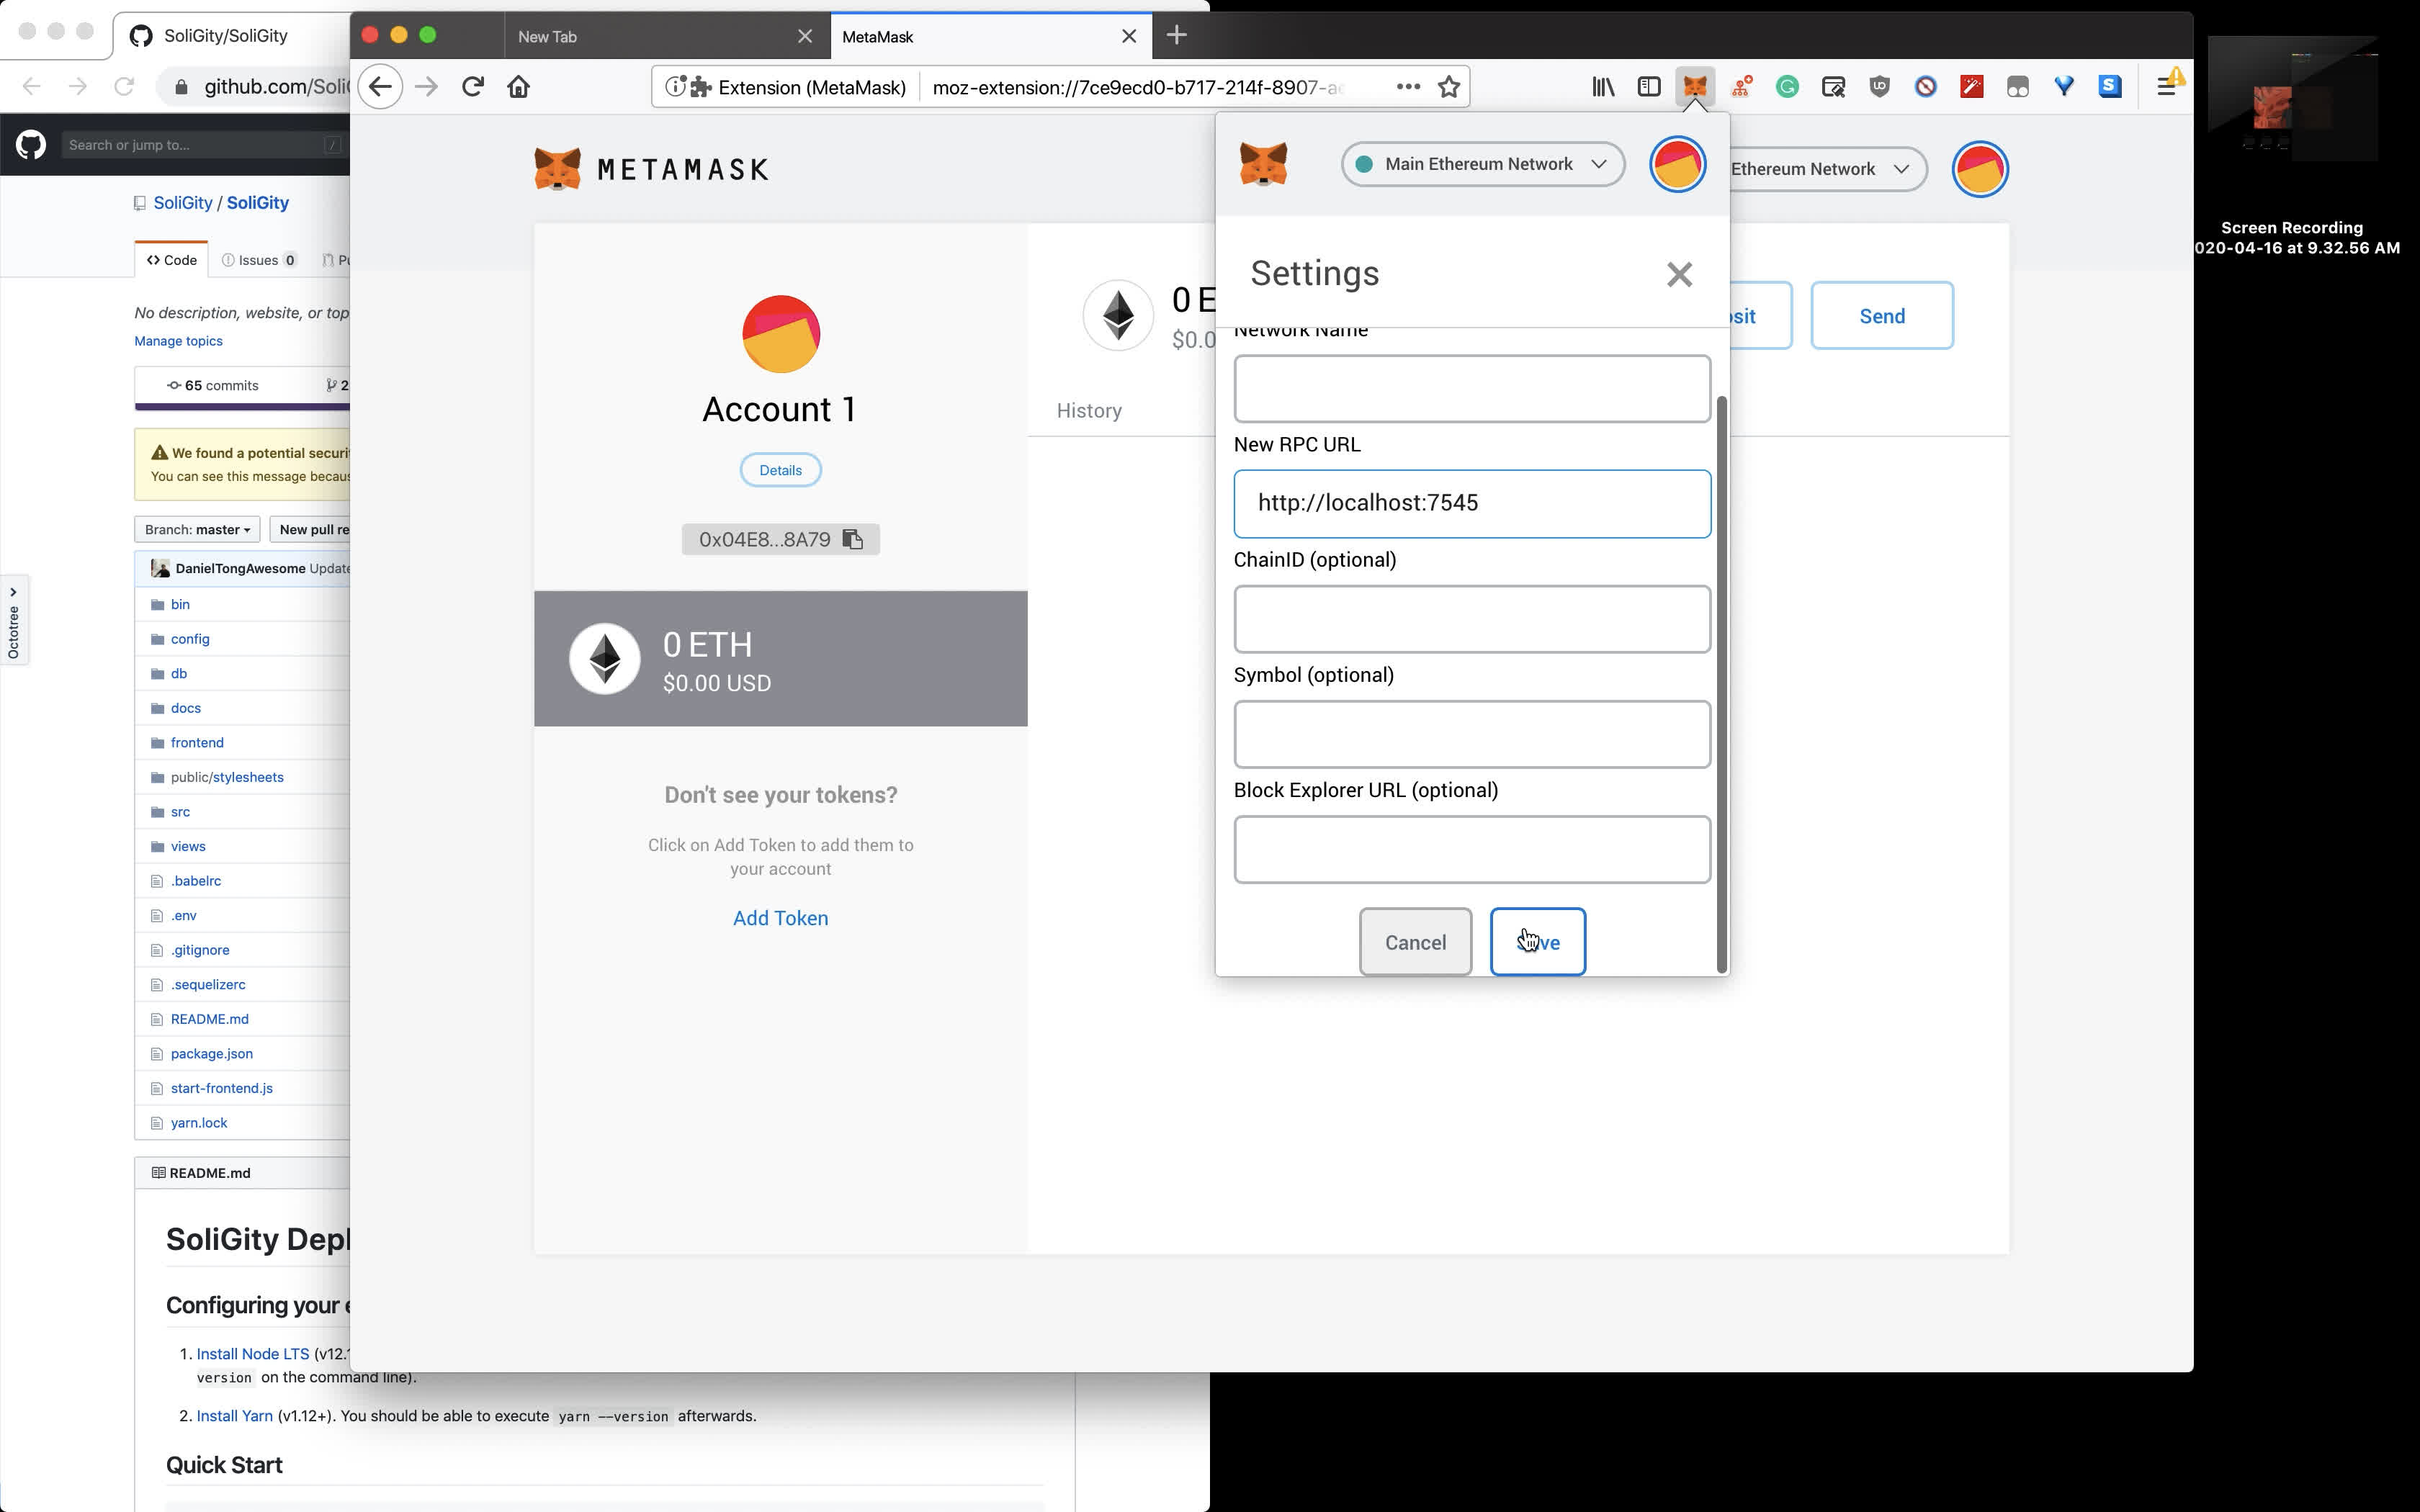
\includegraphics[height=7cm]{graphs/09. metamask_setup_network}

% 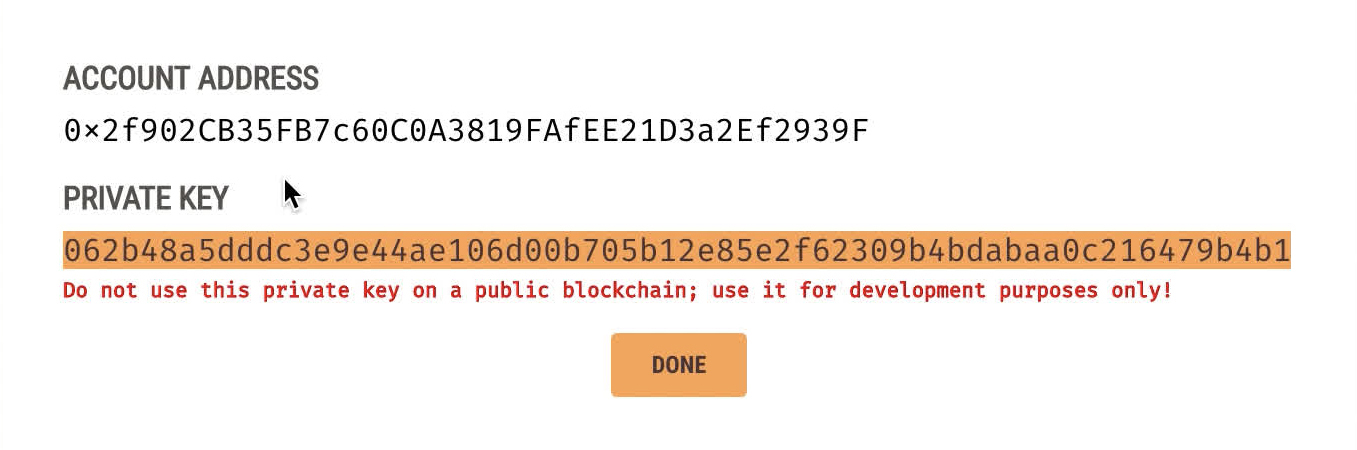
\includegraphics[height=7cm]{graphs/10. metamask_setup_bob}

% 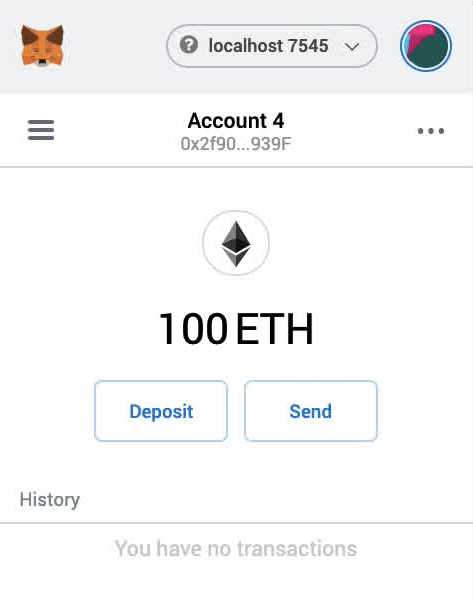
\includegraphics[height=7cm]{graphs/11. metamask_setup_bob}

% 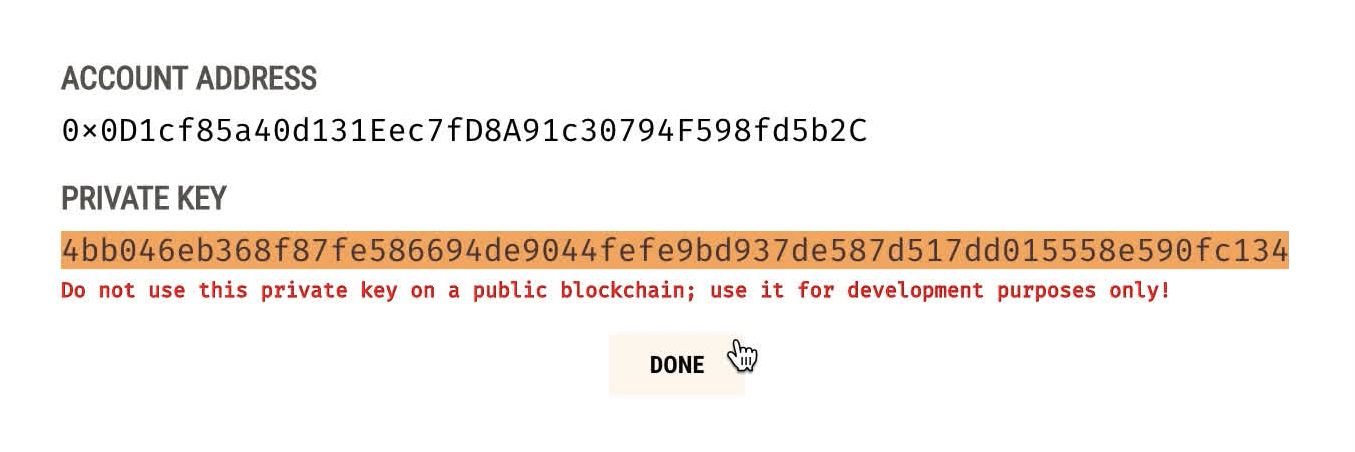
\includegraphics[height=7cm]{graphs/12. metamask_setup_alice}

% 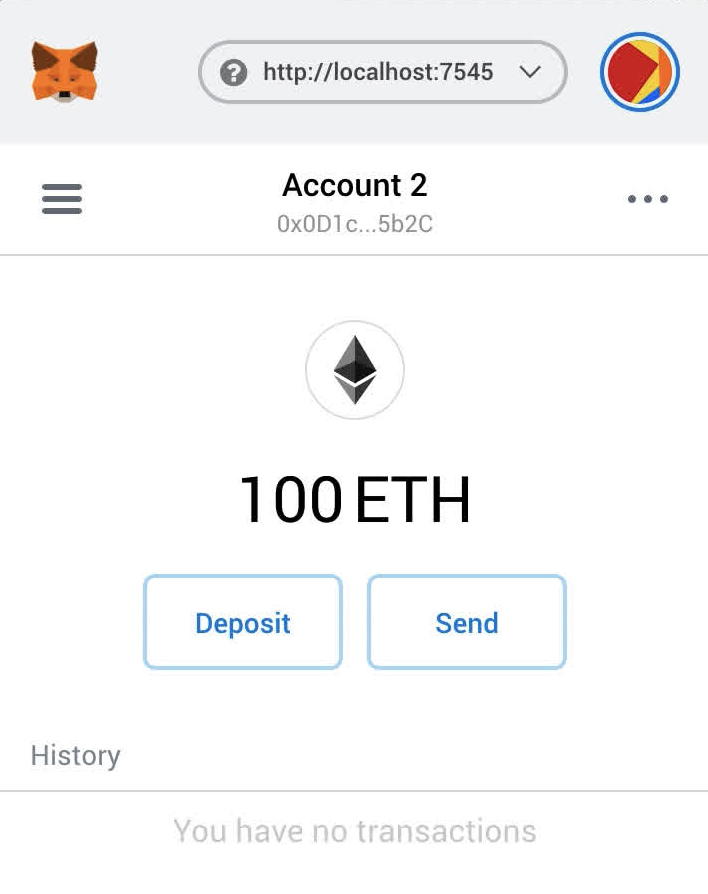
\includegraphics[height=7cm]{graphs/13. metamask_setup_alice}

% 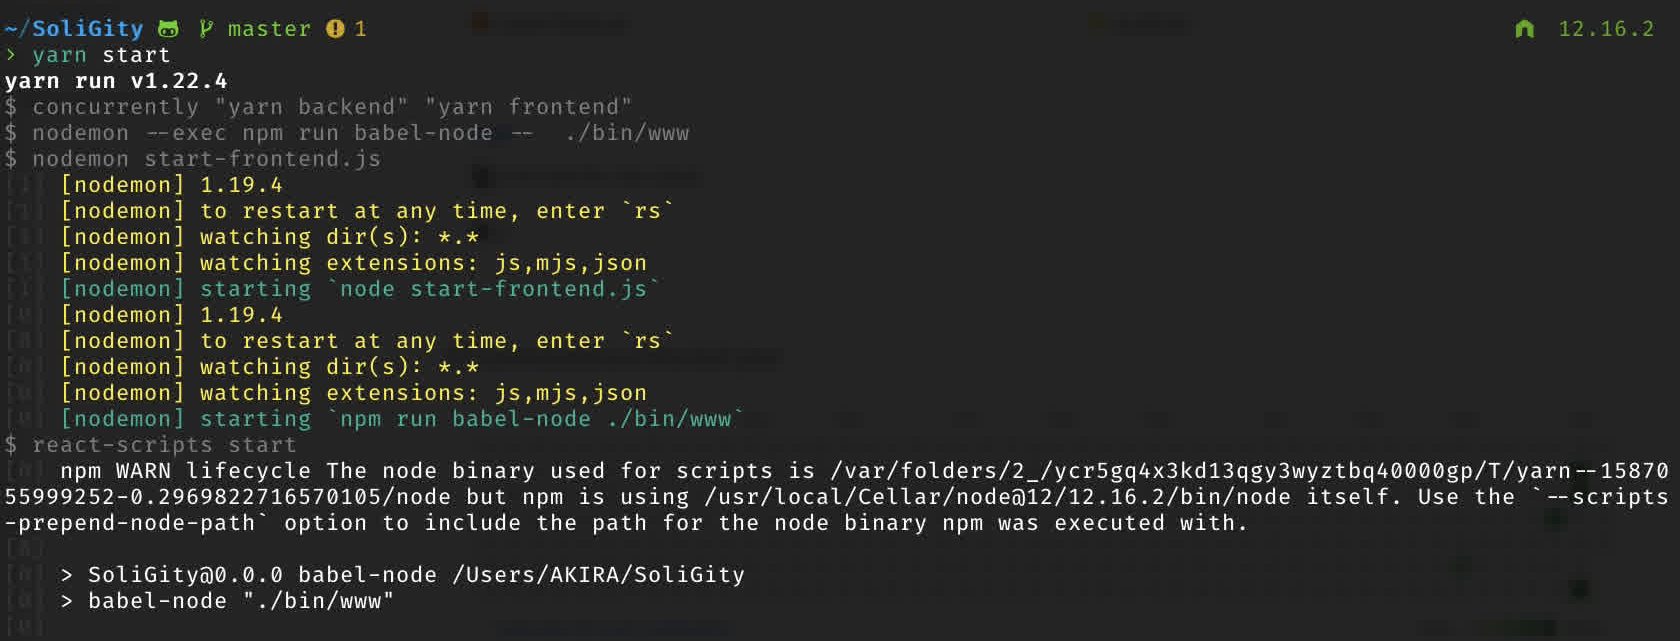
\includegraphics[height=7cm]{graphs/14. yarn_start}

% 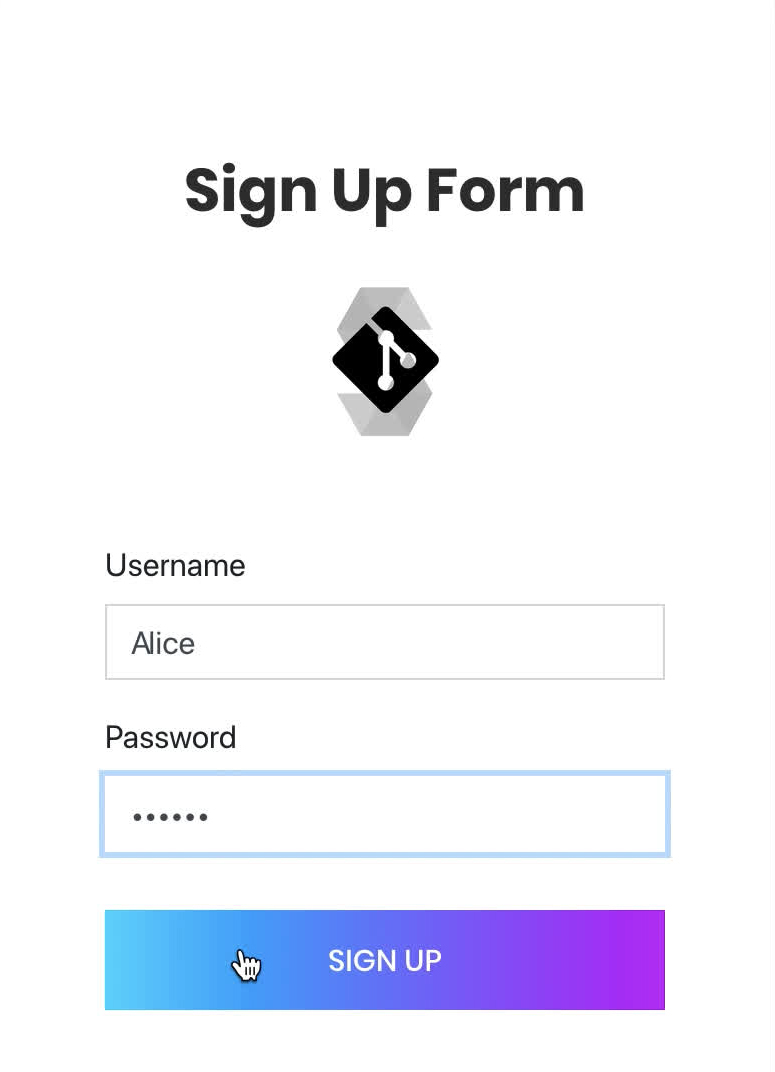
\includegraphics[height=7cm]{graphs/15. alice_sign_up}

% 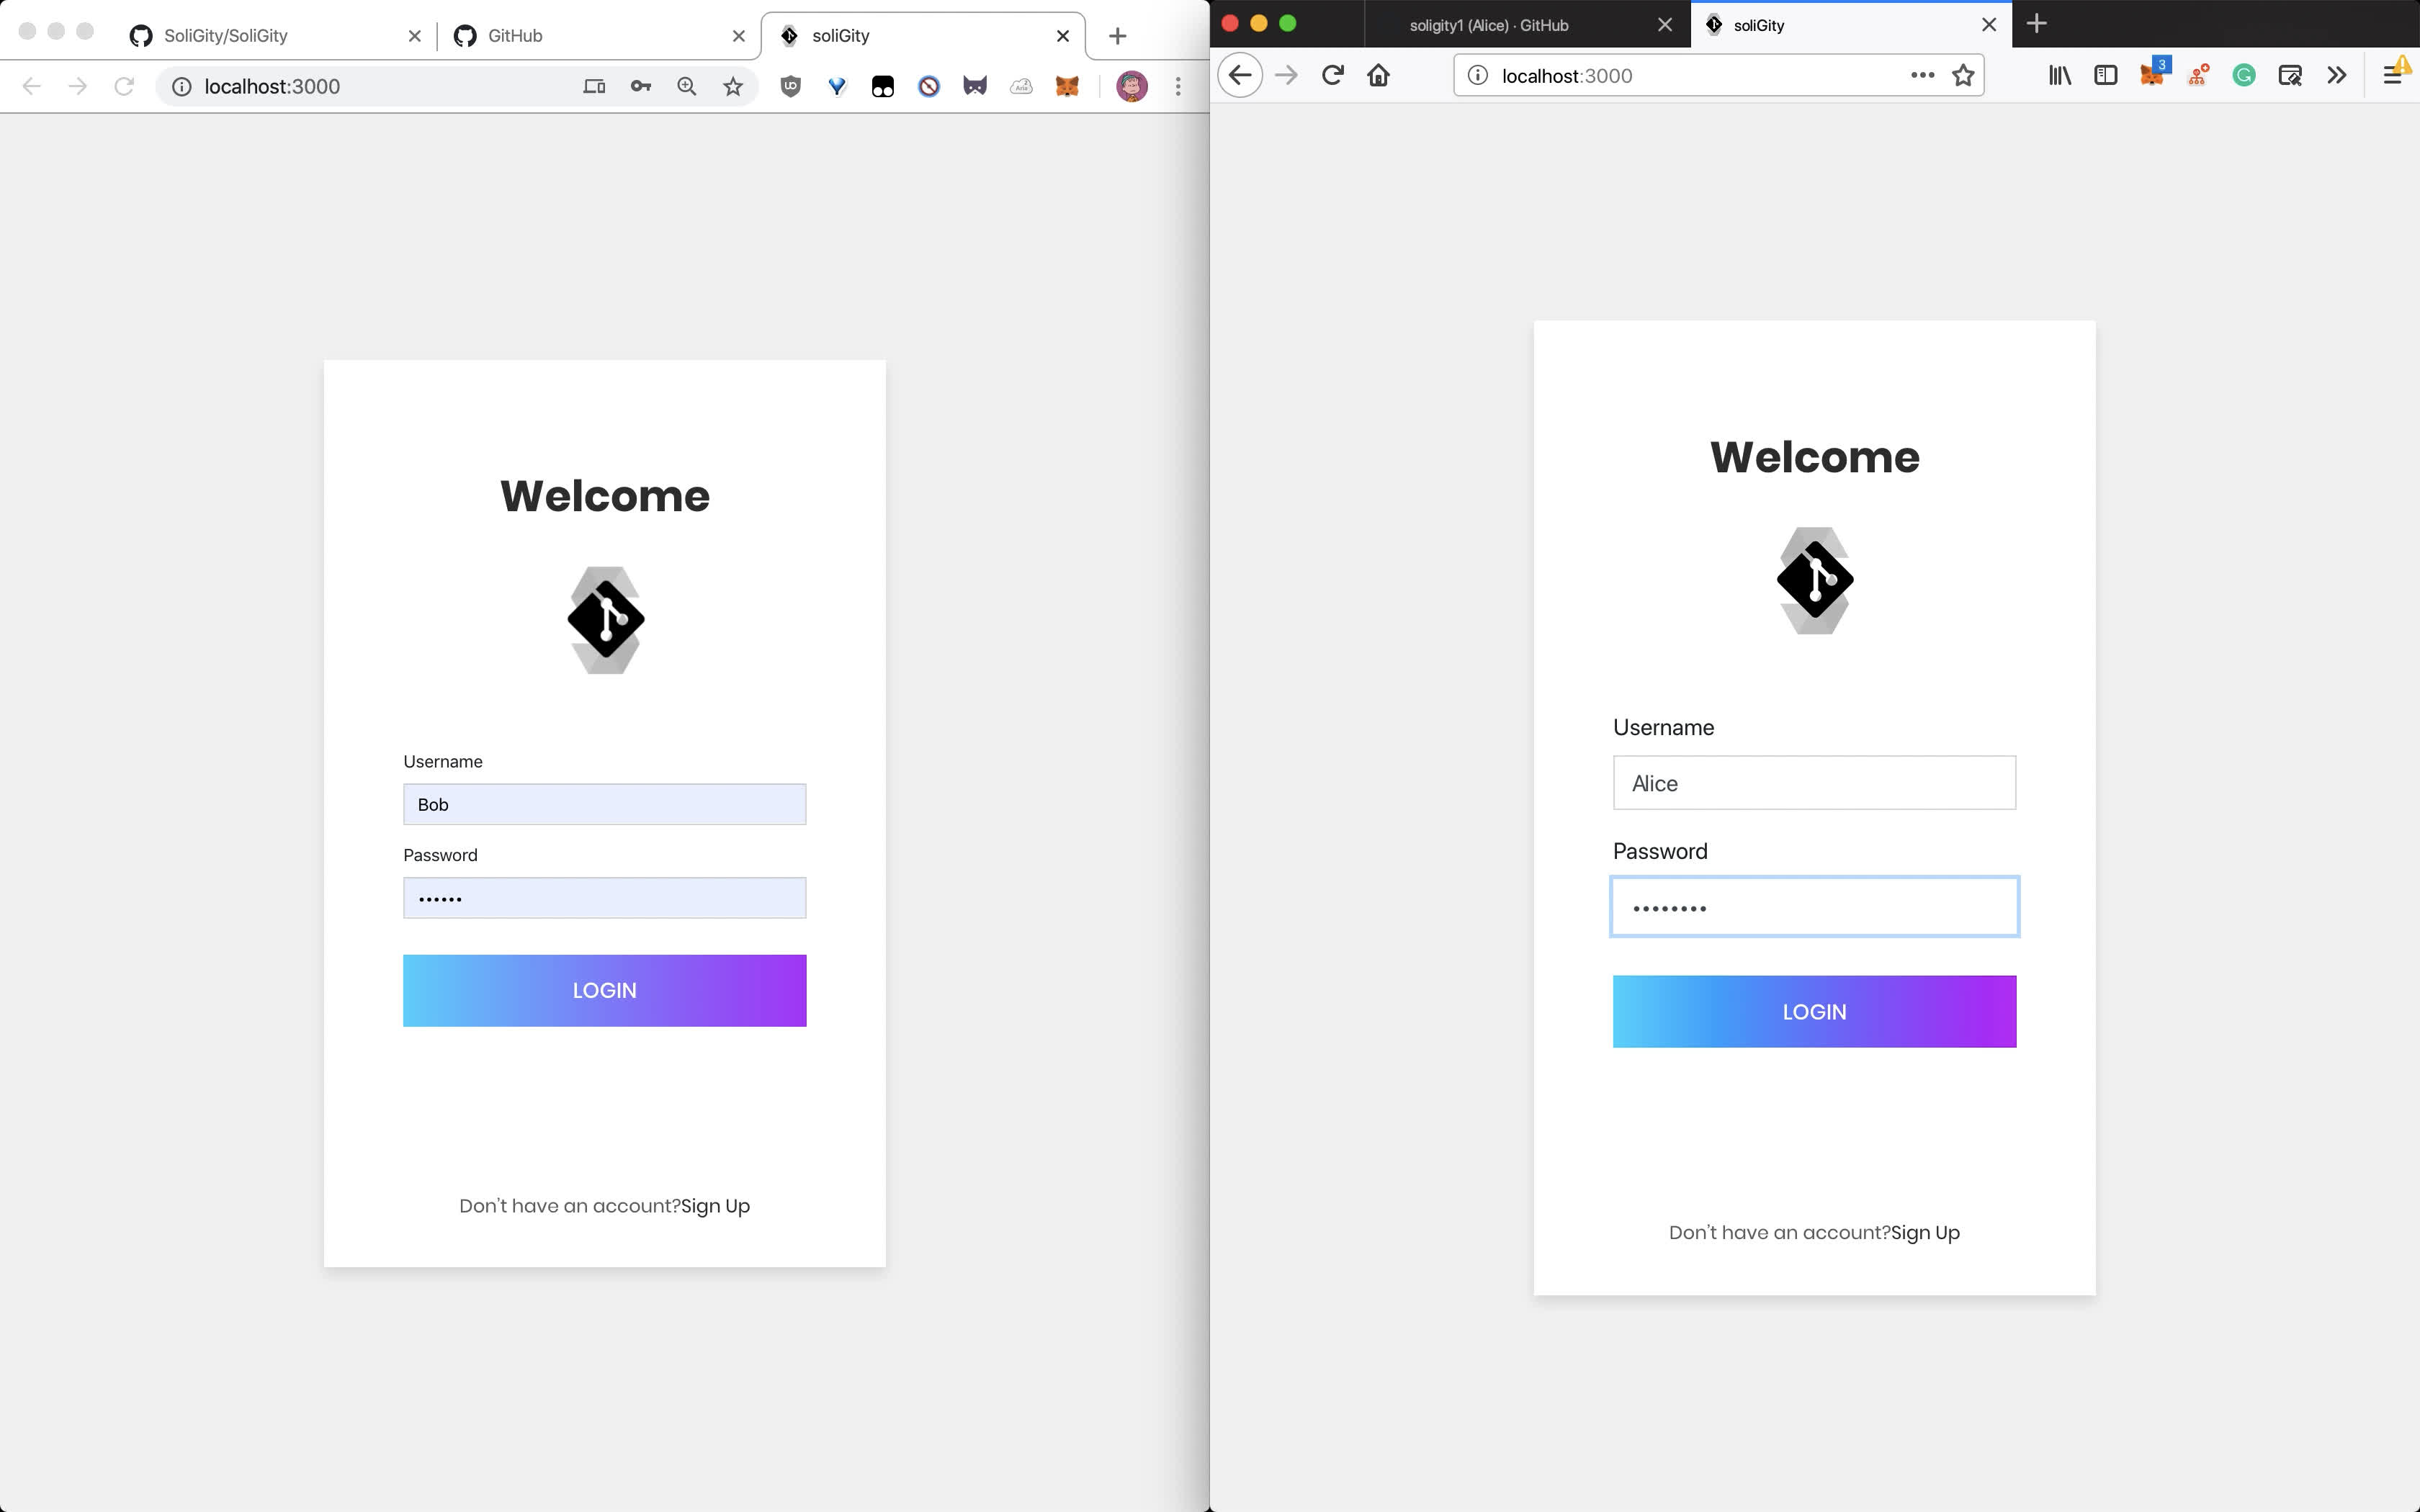
\includegraphics[height=7cm]{graphs/16. alice_login}

% 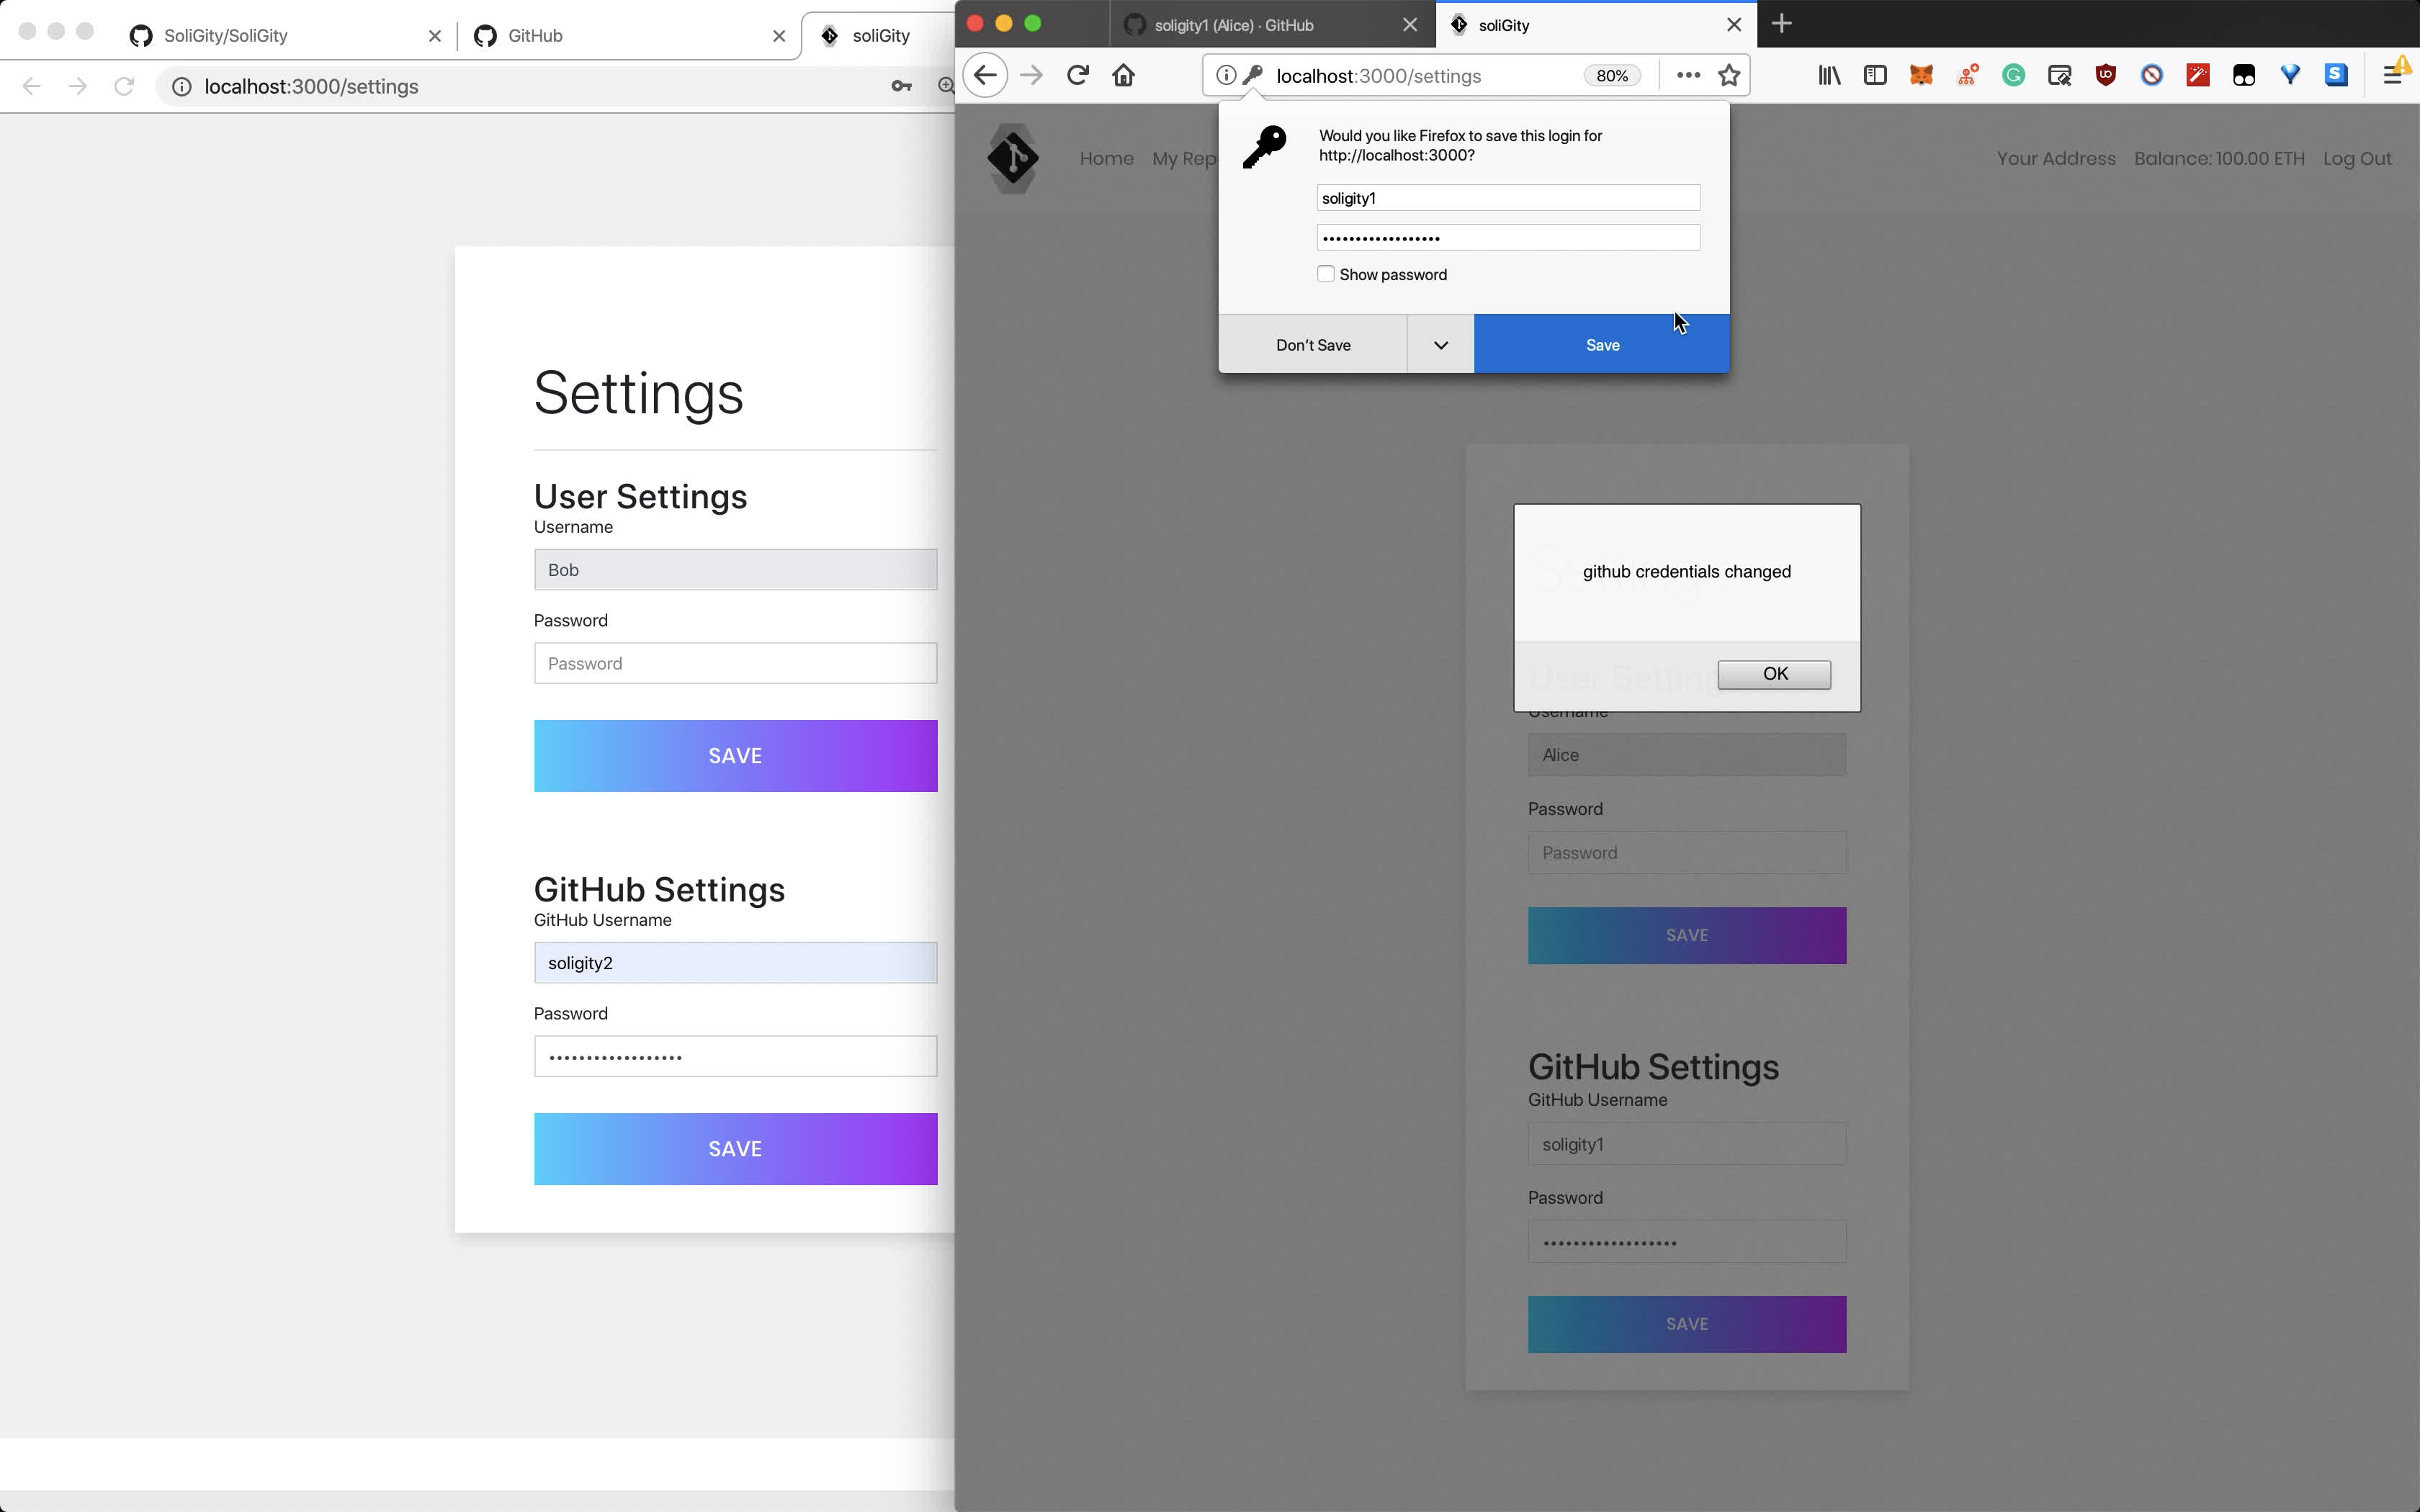
\includegraphics[height=7cm]{graphs/17. alice_gitub_setup}

% 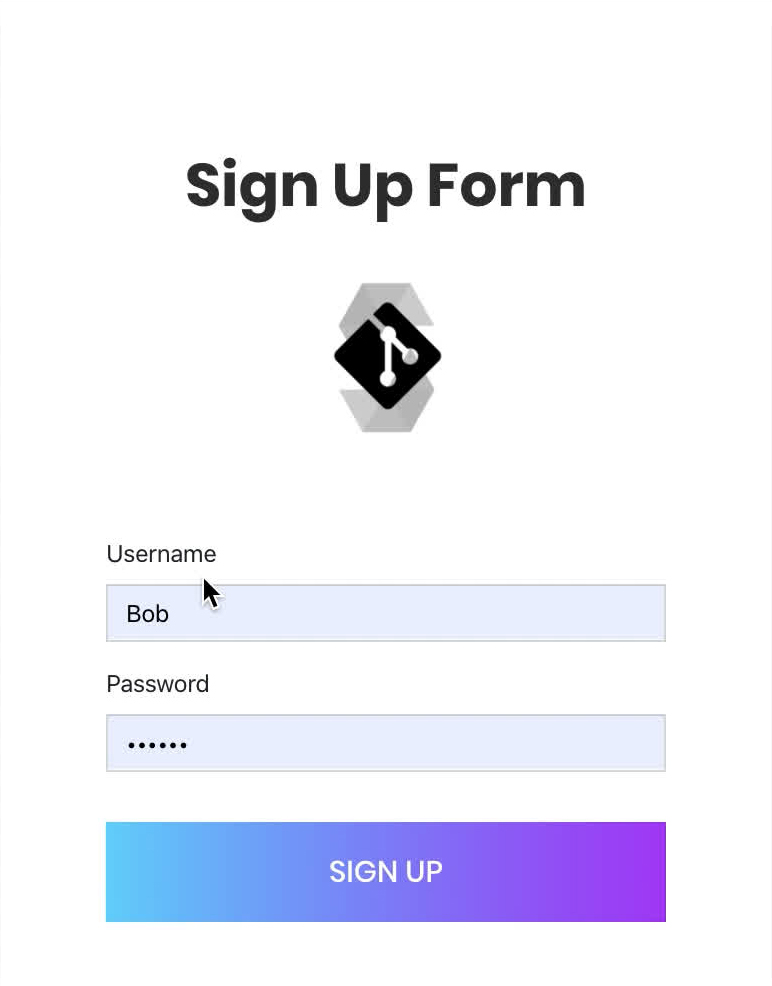
\includegraphics[height=7cm]{graphs/18. bob_sign_up}

% 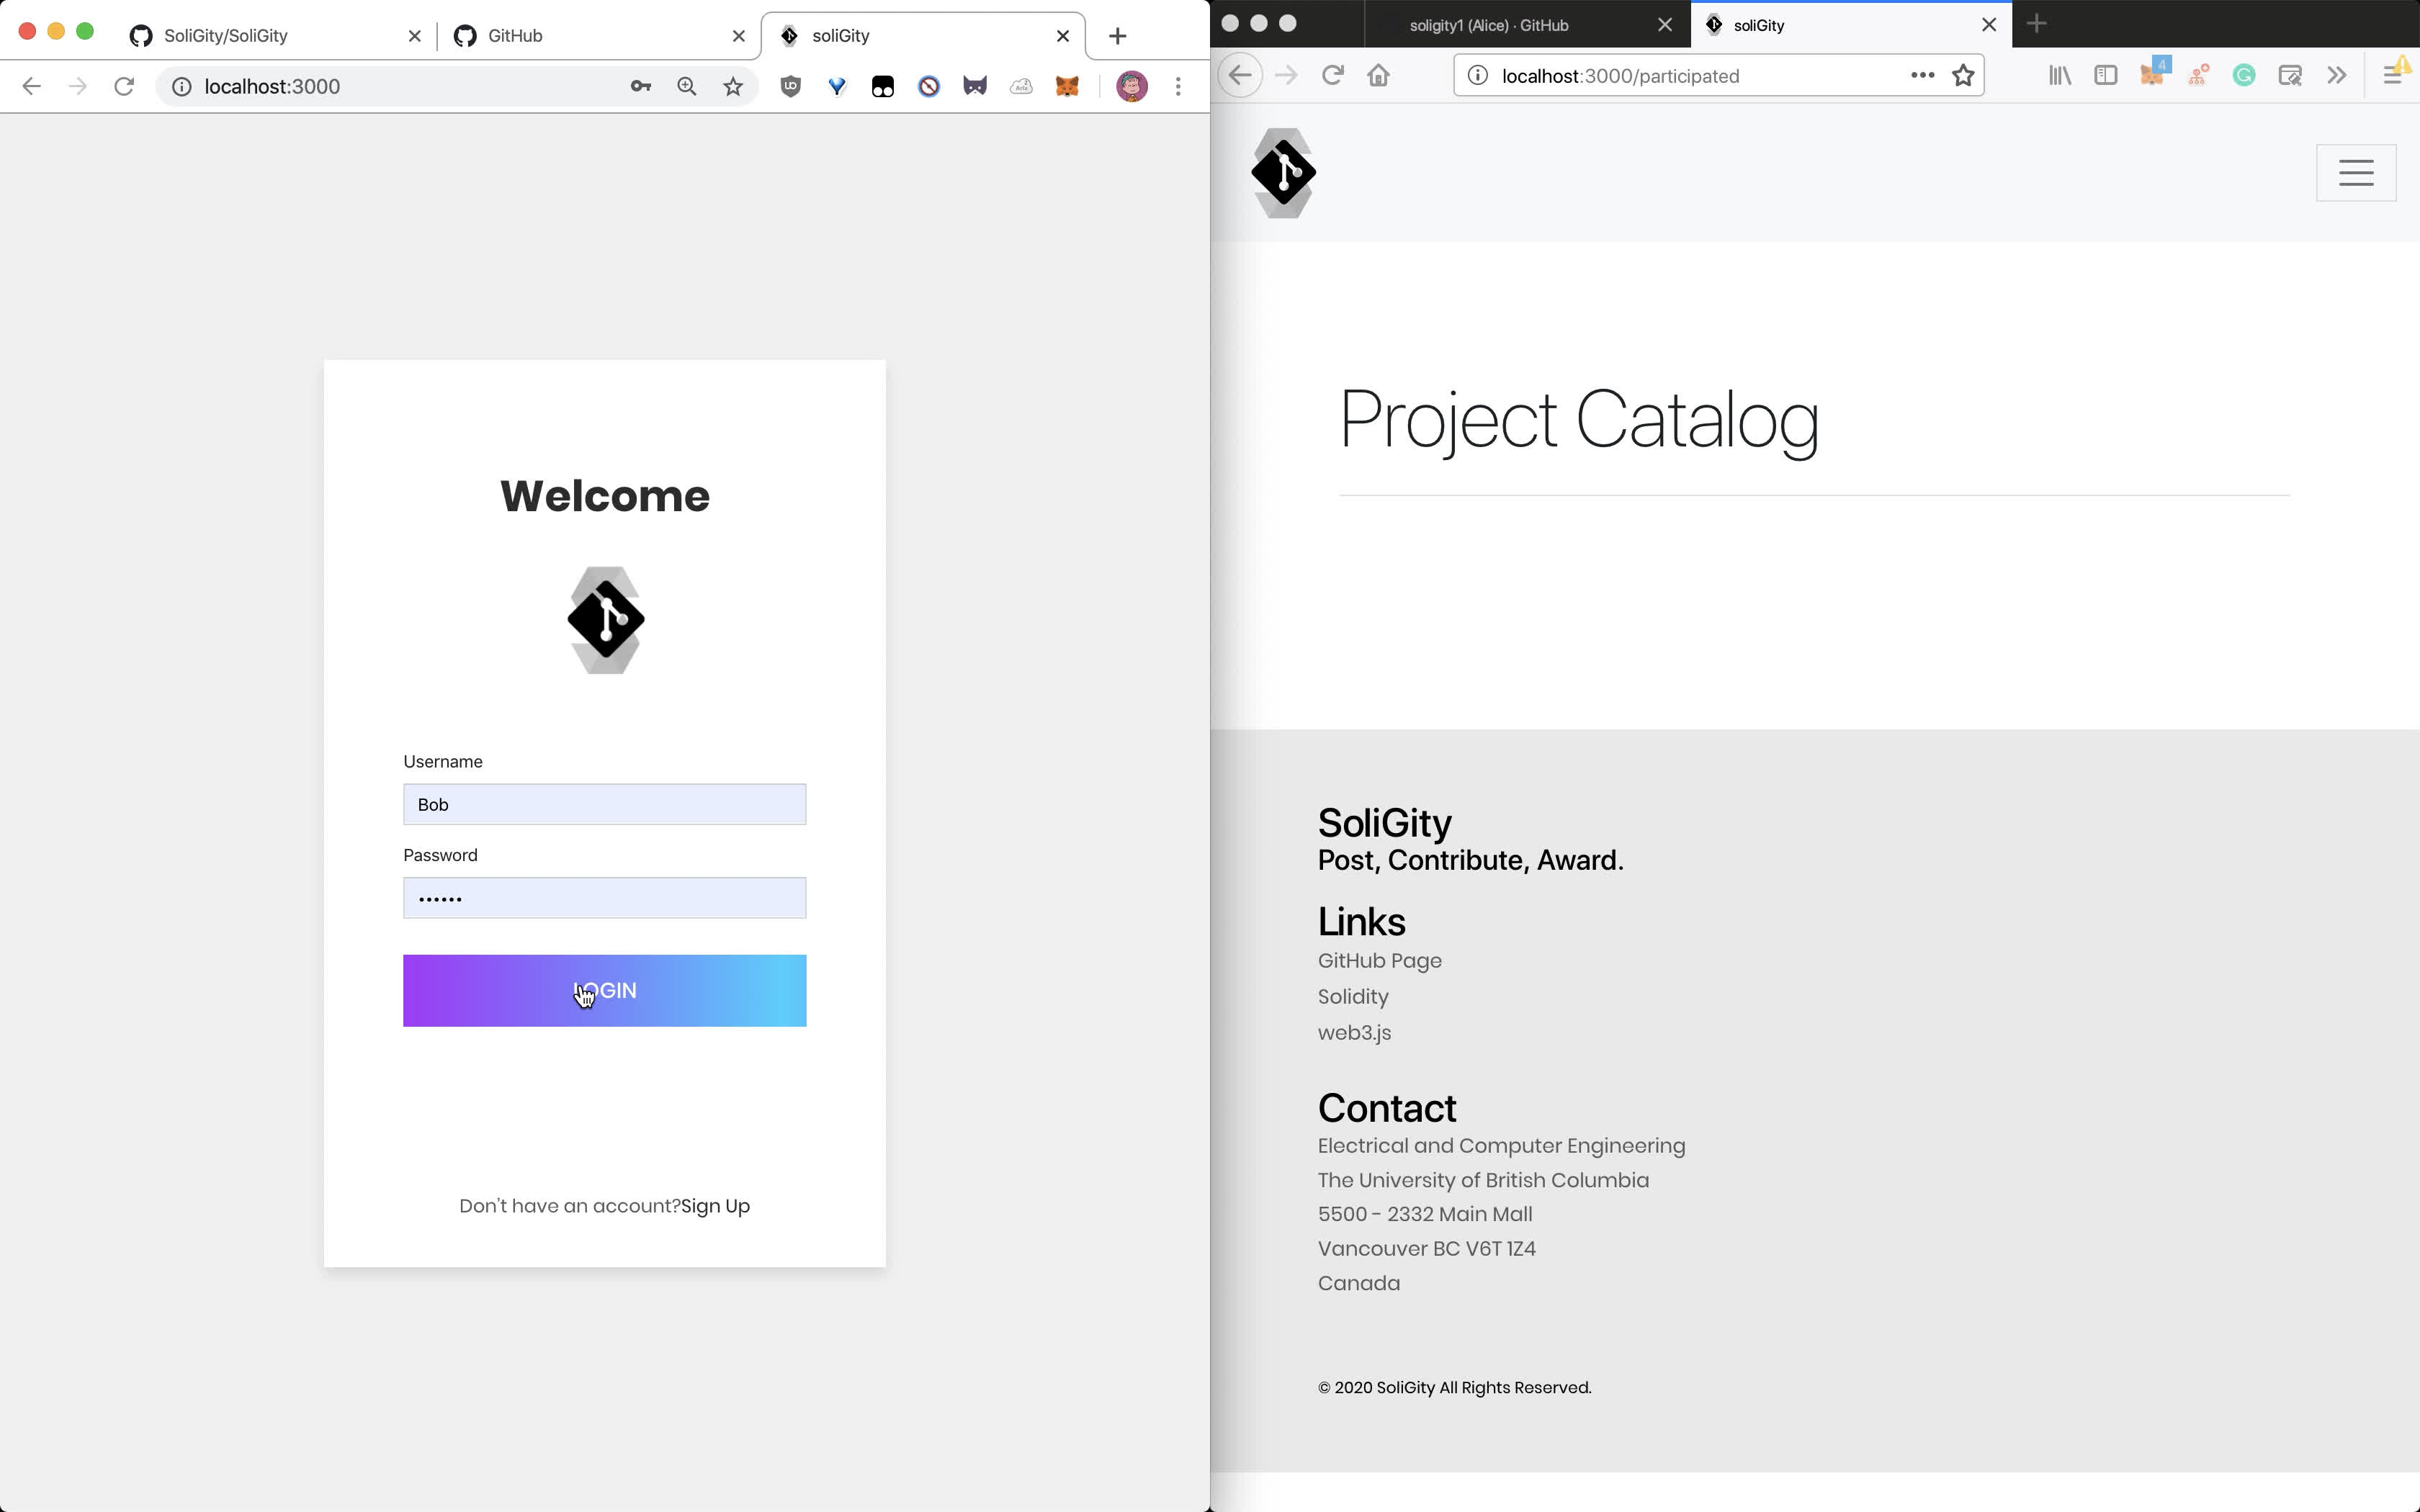
\includegraphics[height=7cm]{graphs/19. bob_login}

% 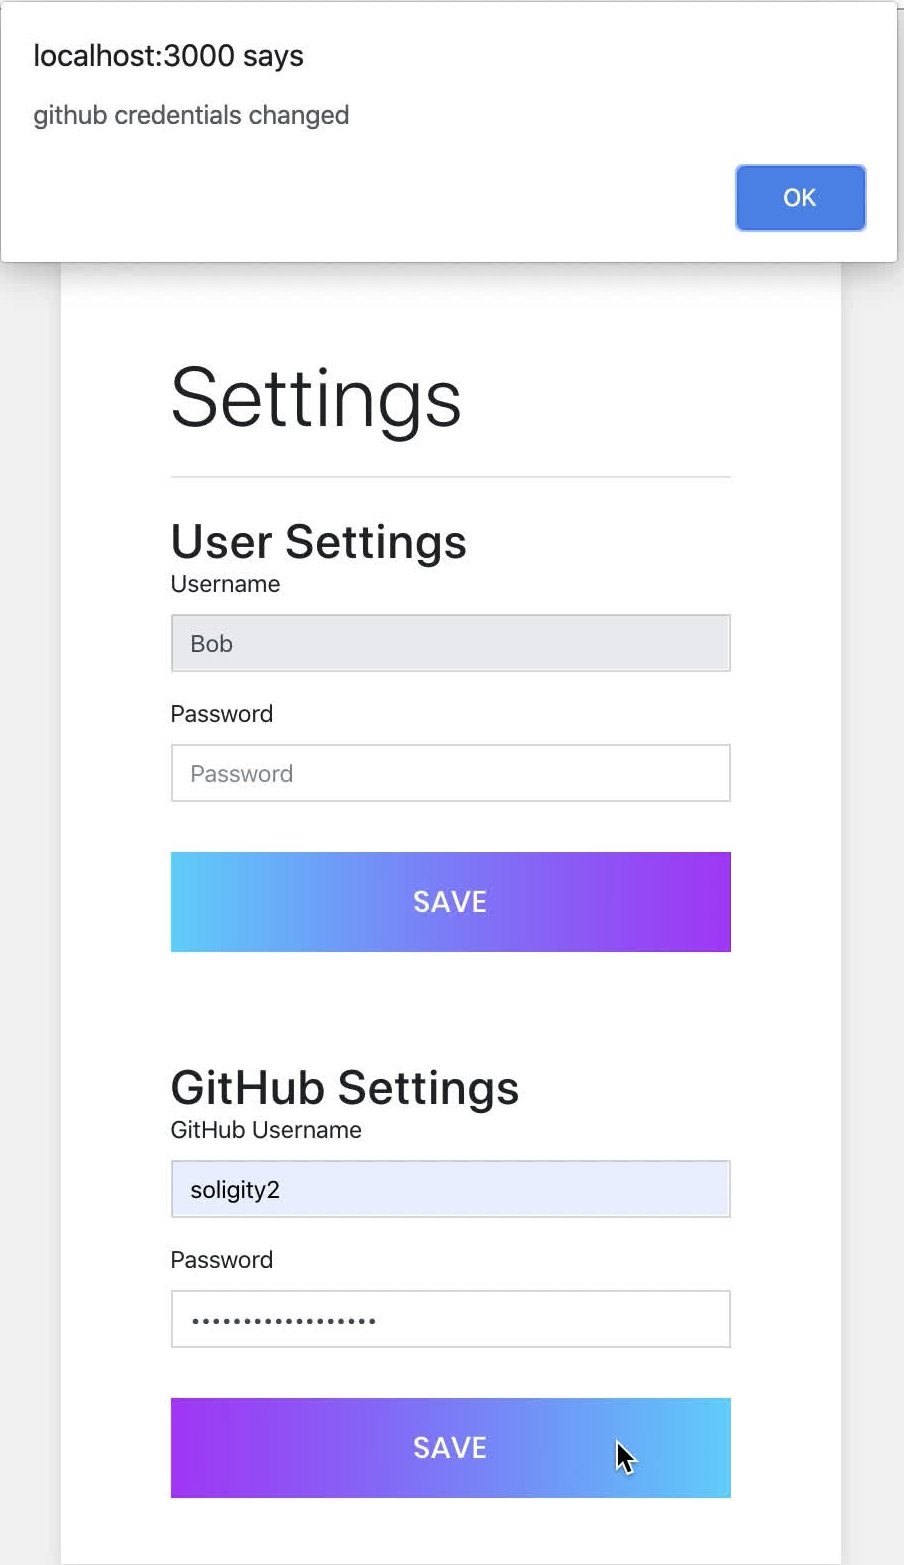
\includegraphics[height=7cm]{graphs/20. bob_gitub_setup}

% 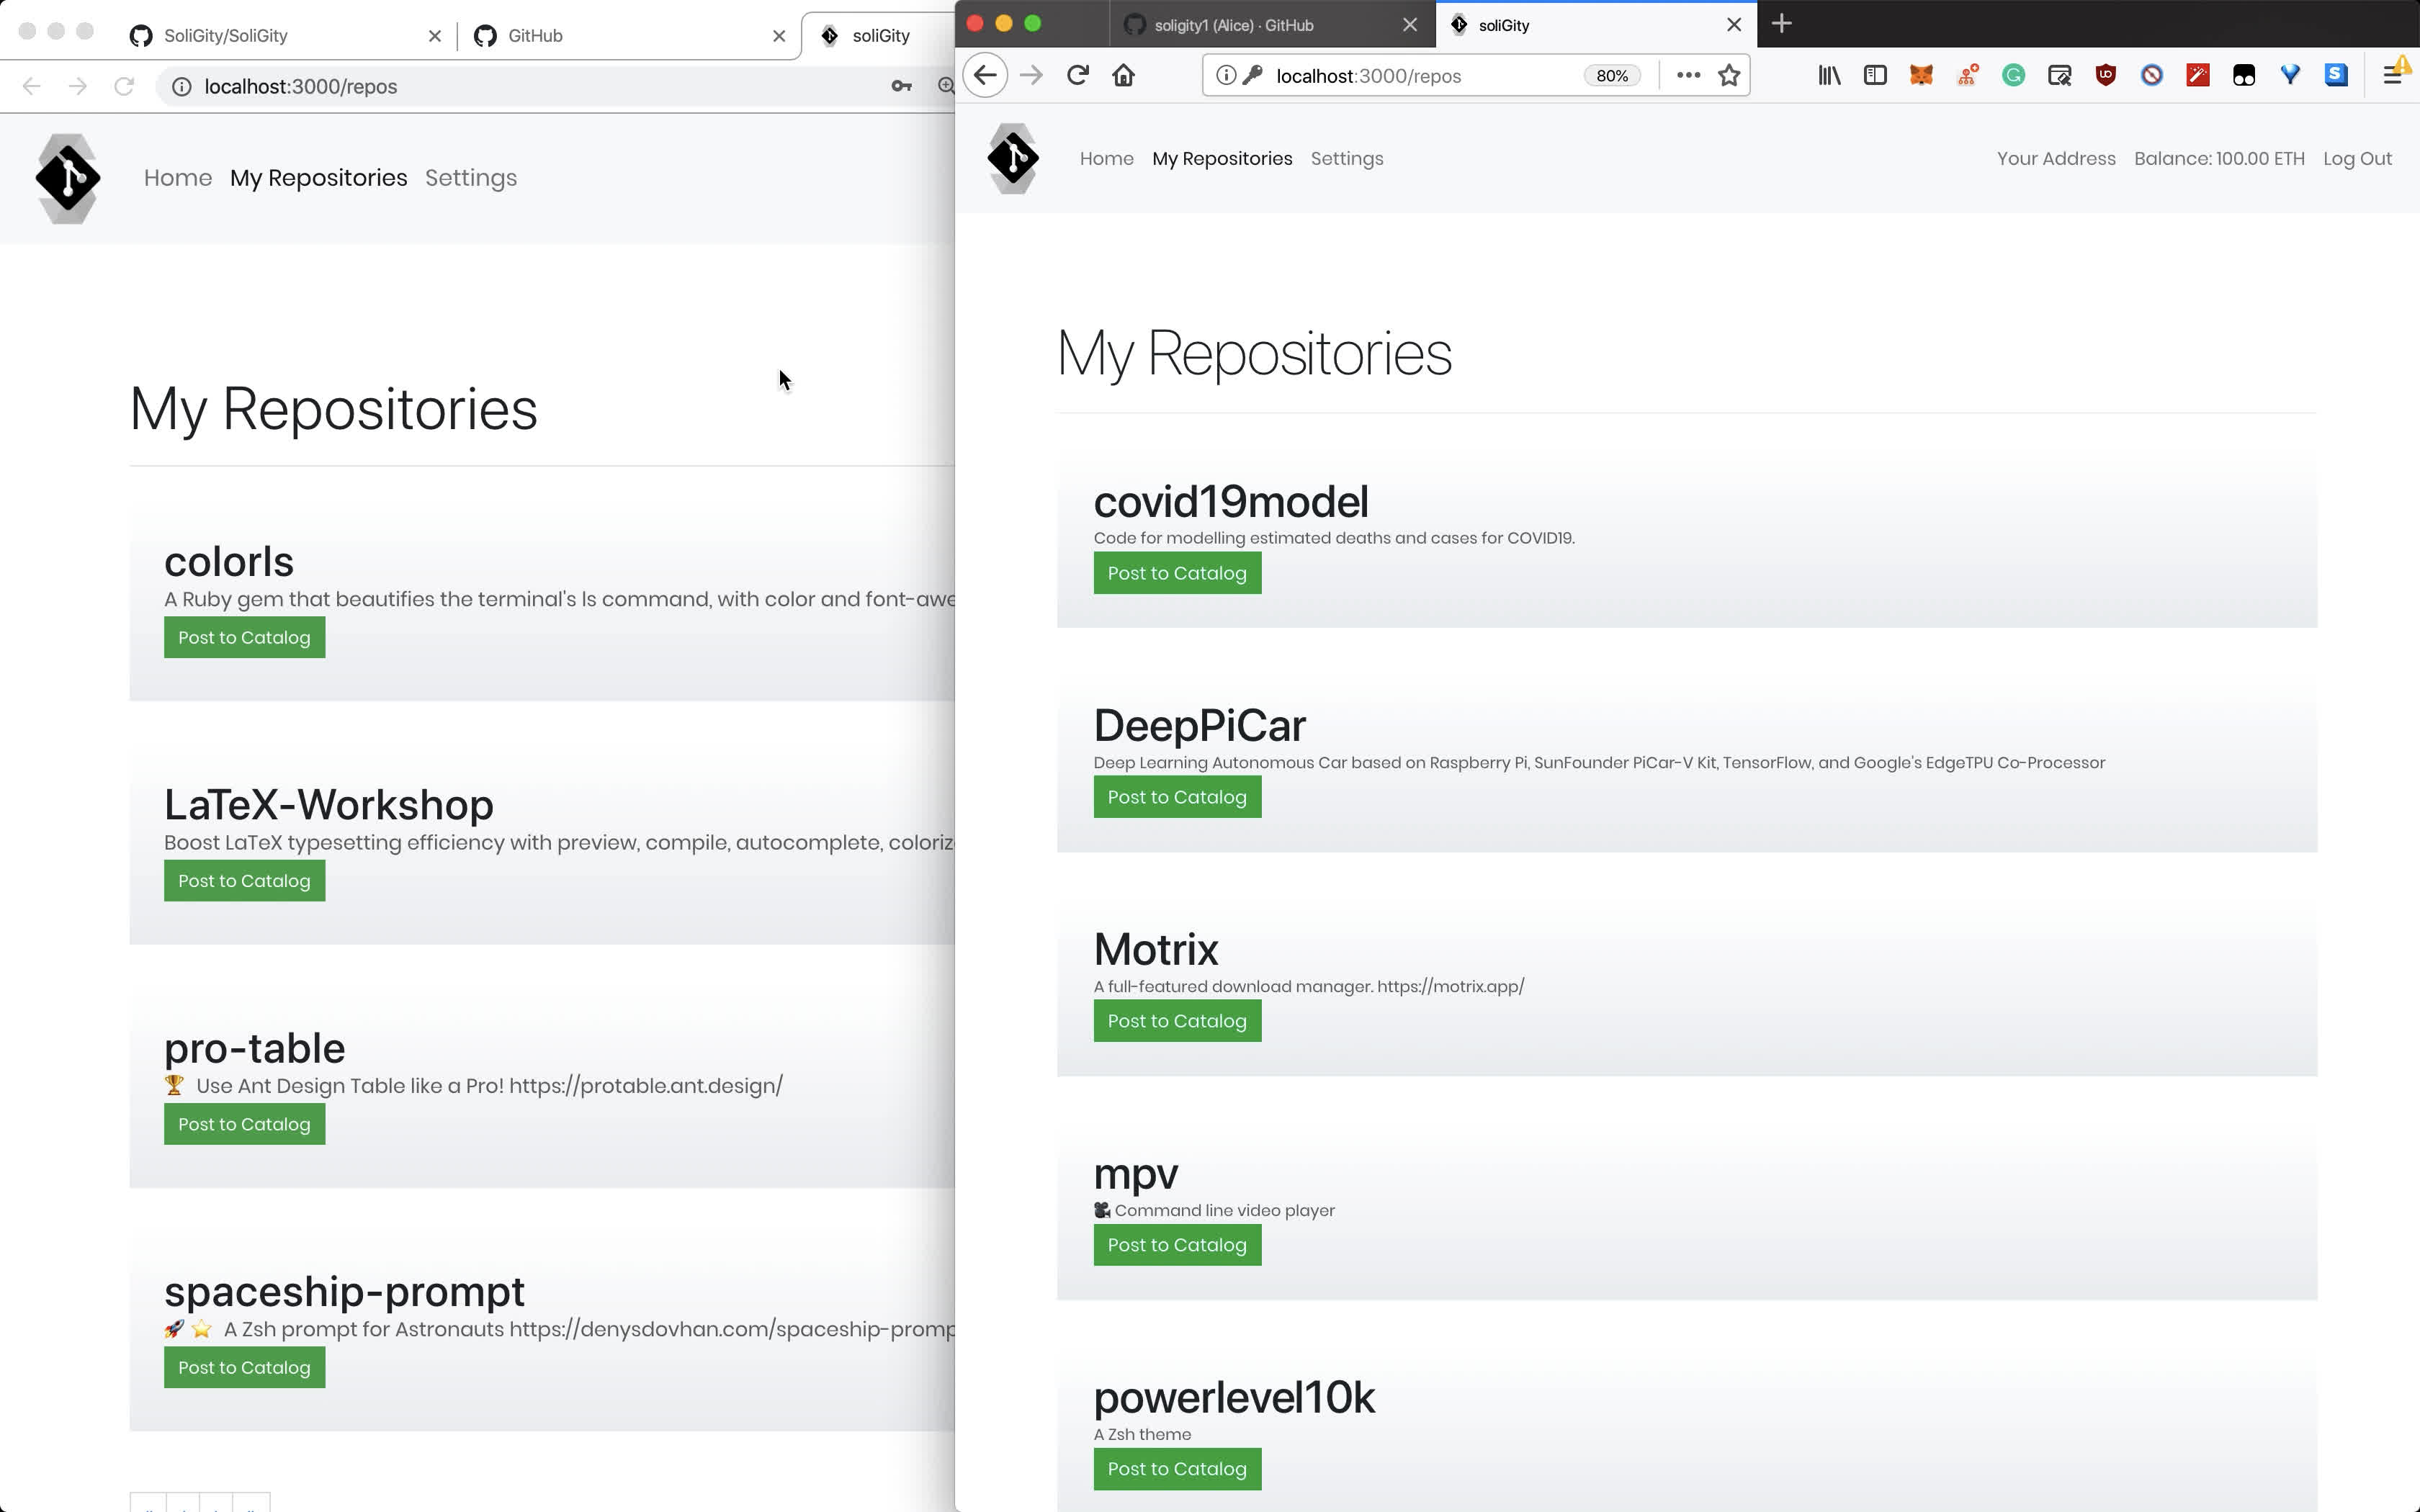
\includegraphics[height=7cm]{graphs/21. alice_bob_repos}

% 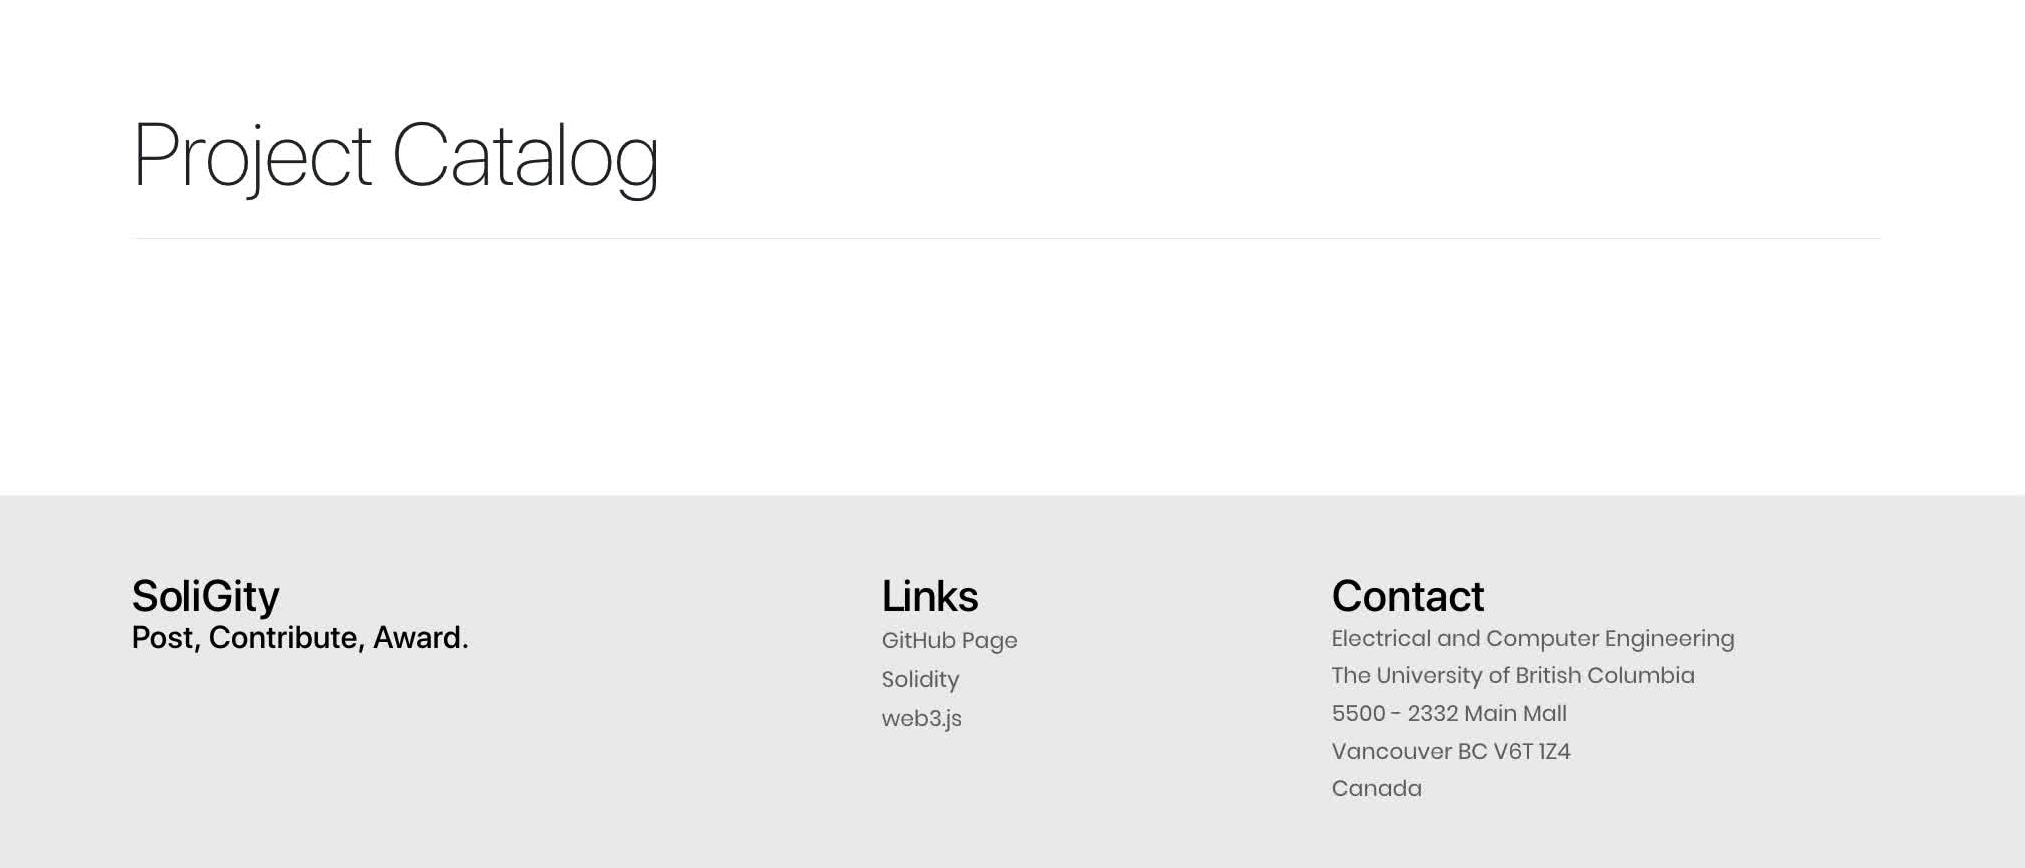
\includegraphics[height=7cm]{graphs/22. empty_project_catalog}

% 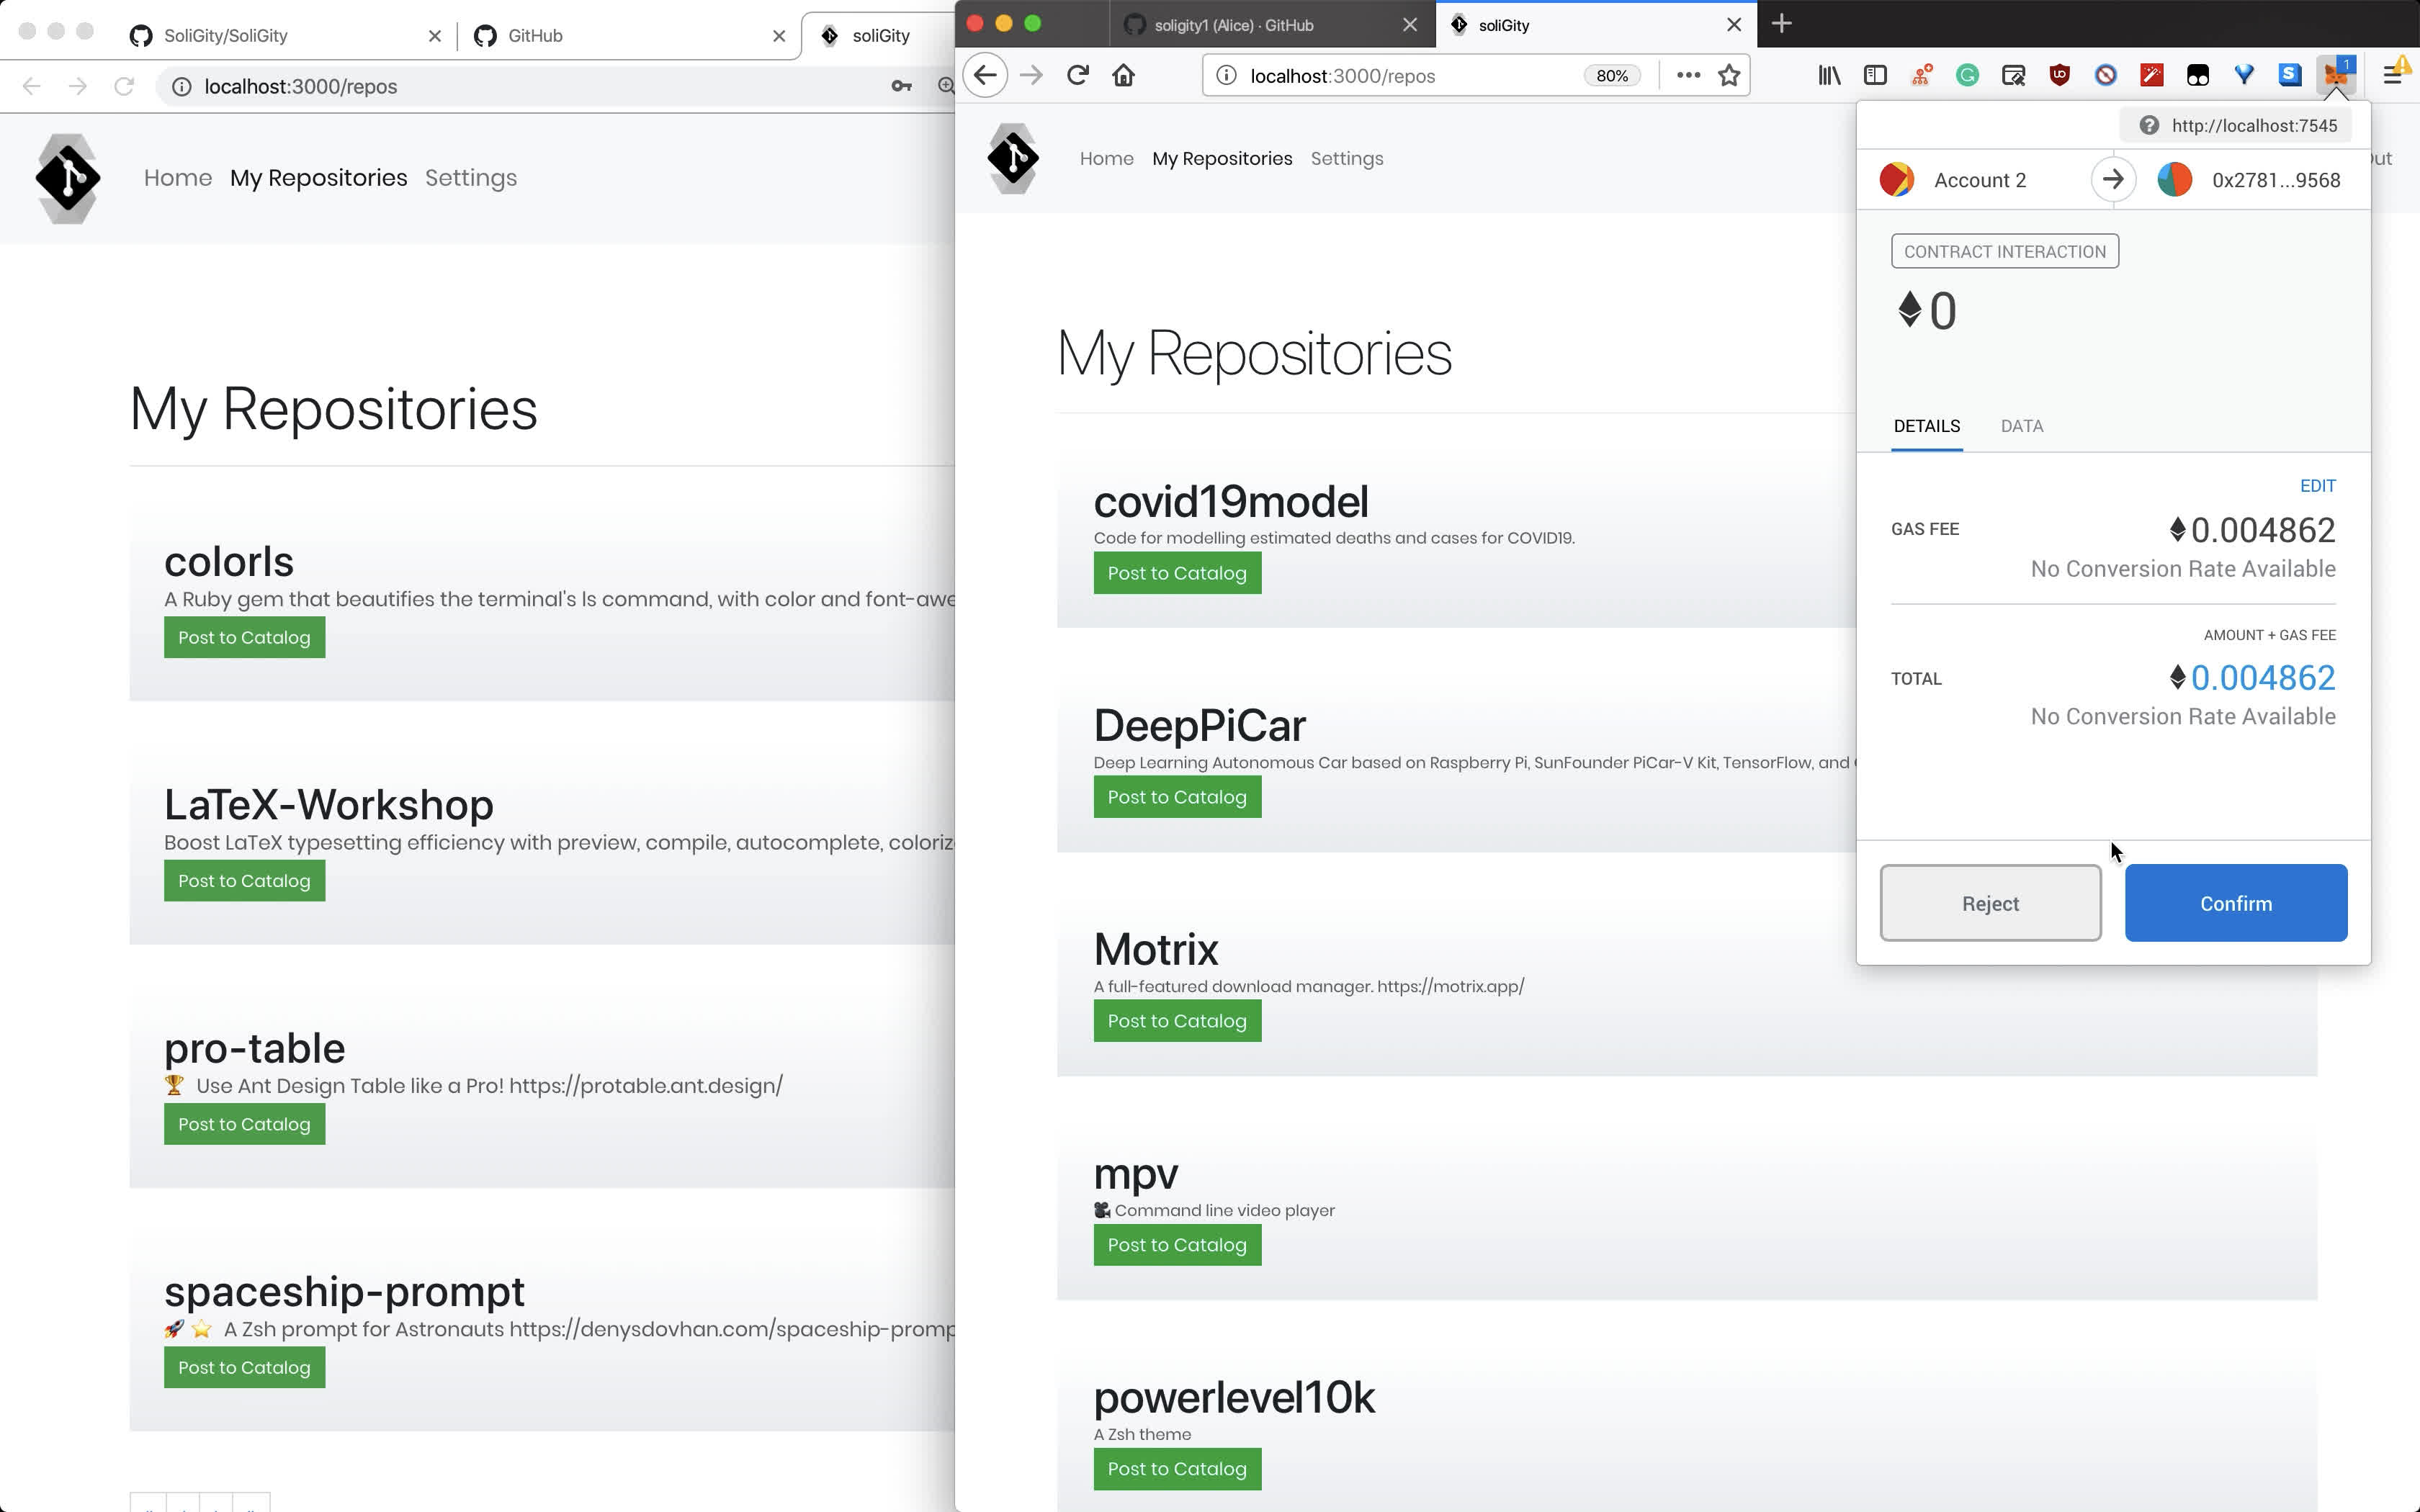
\includegraphics[height=7cm]{graphs/23. alice_post_to_catalog_1}

% 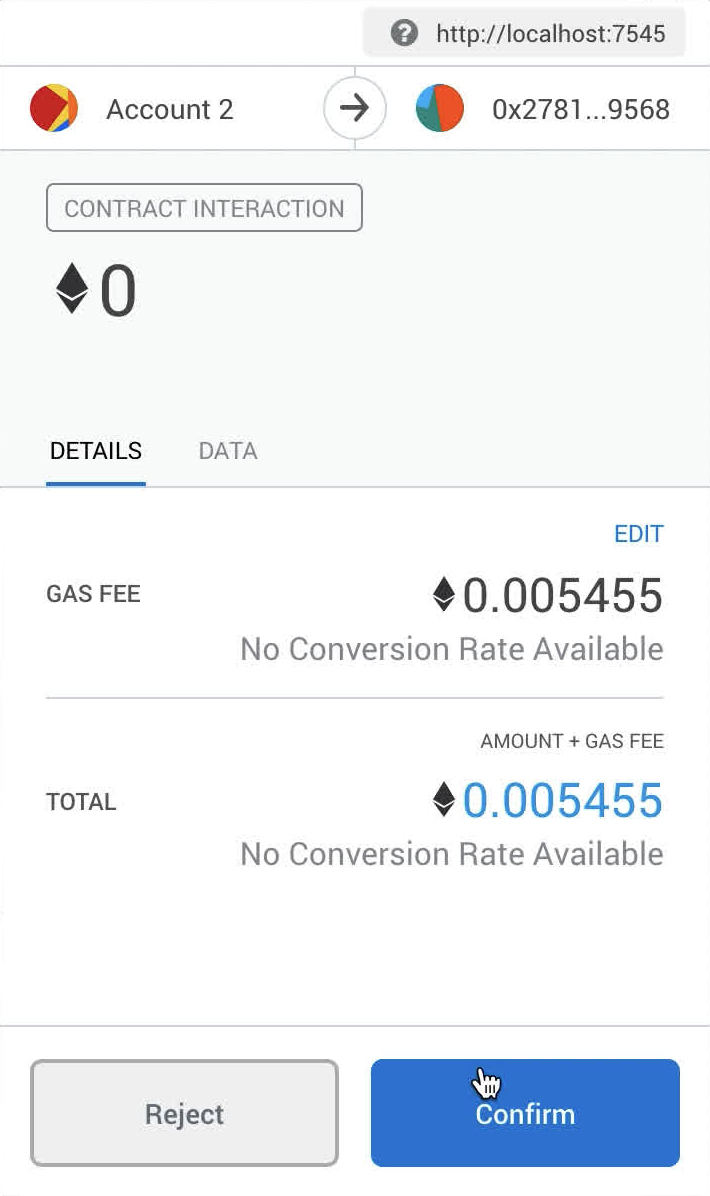
\includegraphics[height=7cm]{graphs/24. alice_post_to_catalog_2}

% 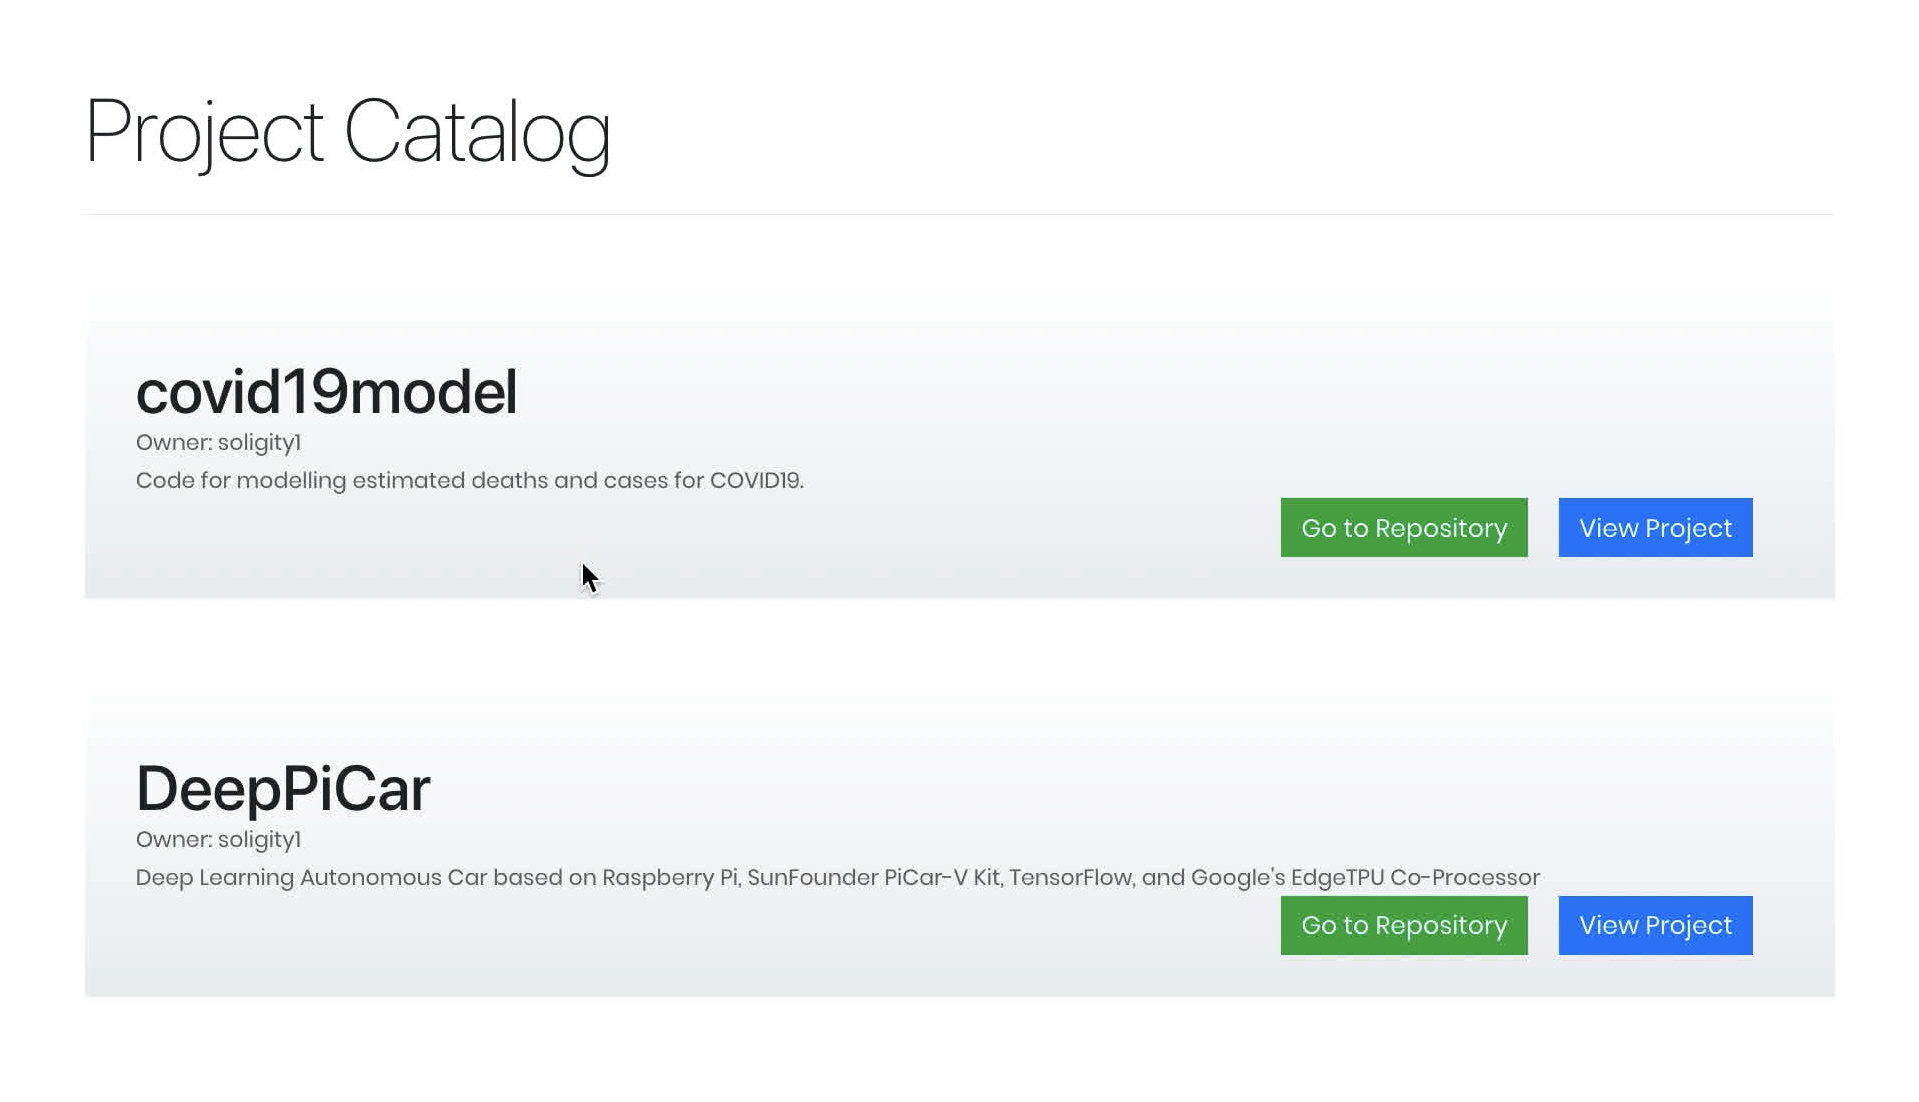
\includegraphics[height=7cm]{graphs/25. added_project_catalog}

% 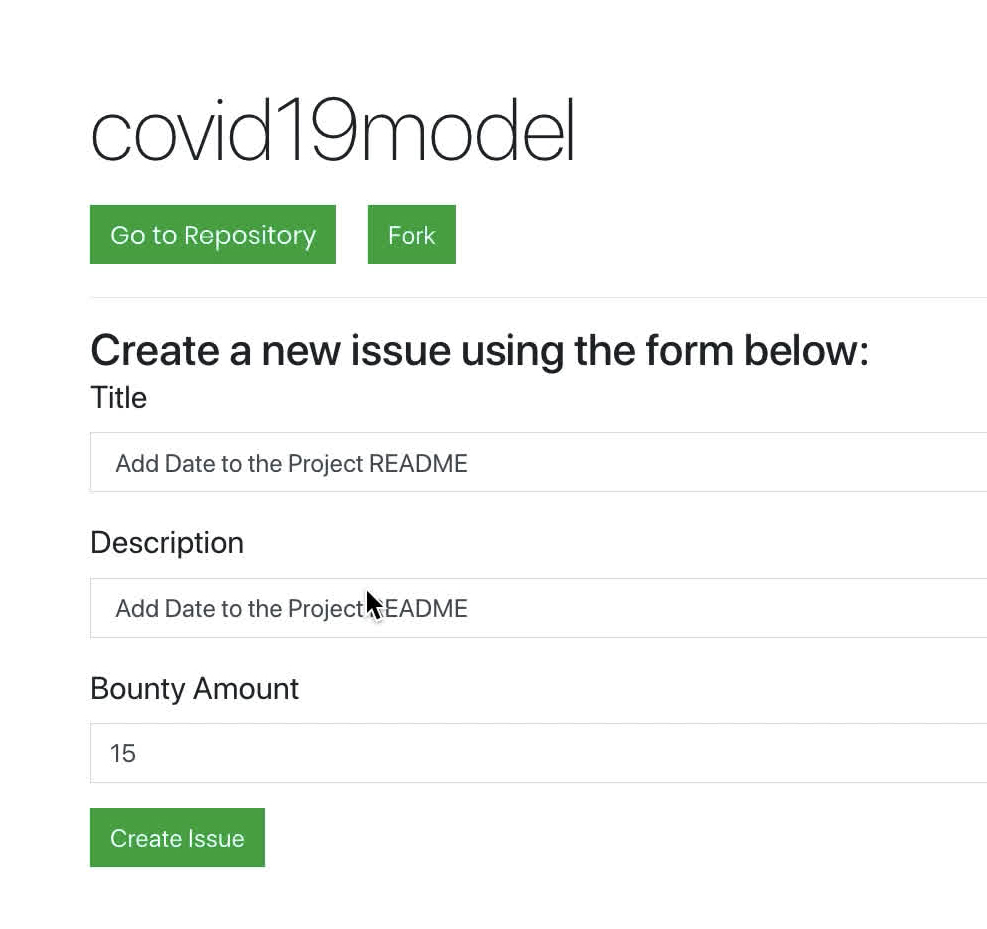
\includegraphics[height=7cm]{graphs/26. alice_create_issue1}

% 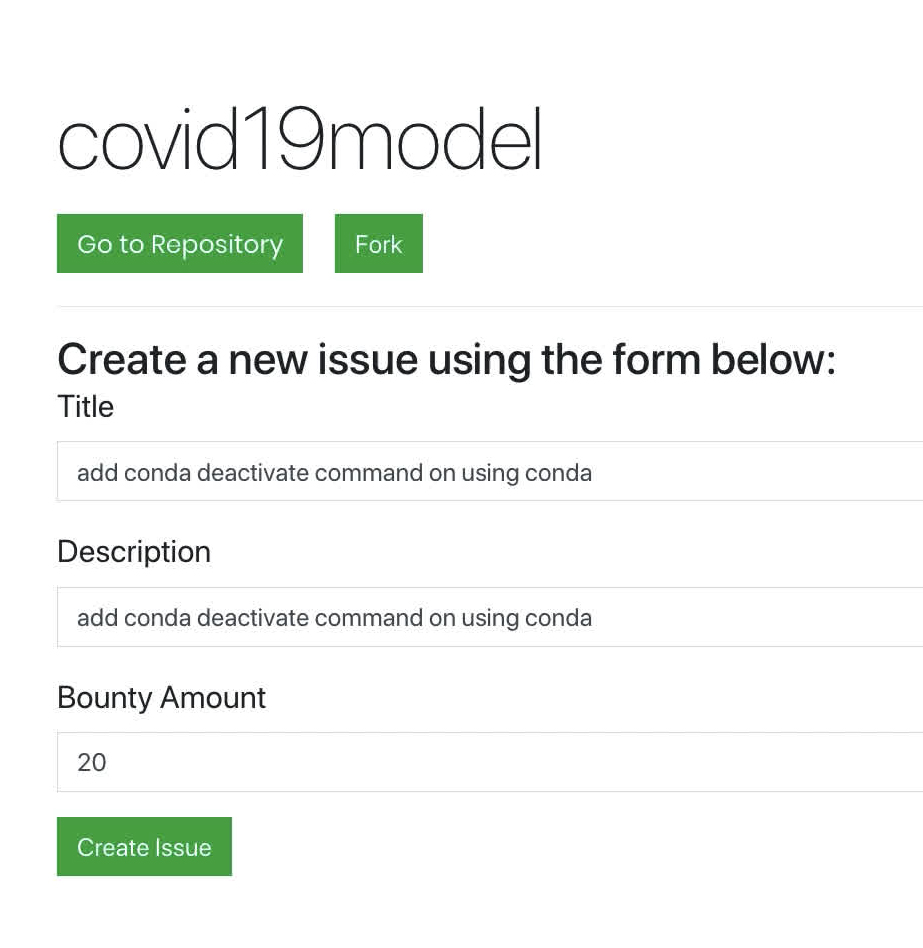
\includegraphics[height=7cm]{graphs/27. alice_create_issue2}

% 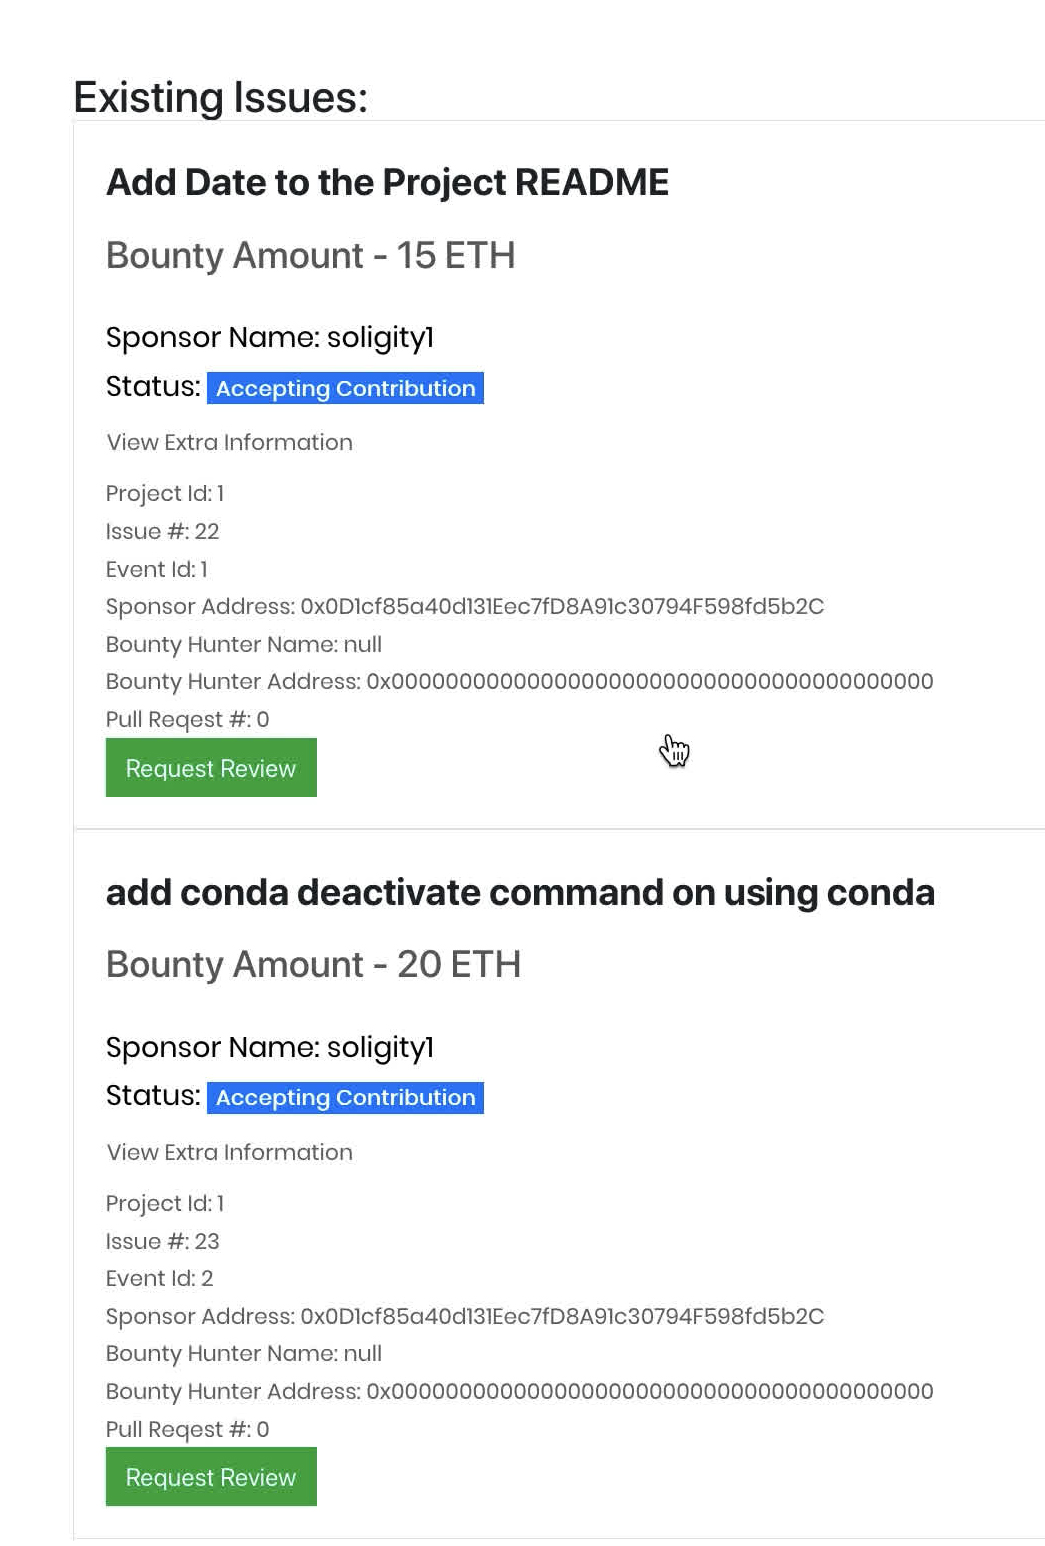
\includegraphics[height=7cm]{graphs/28. soligity_issues}

% 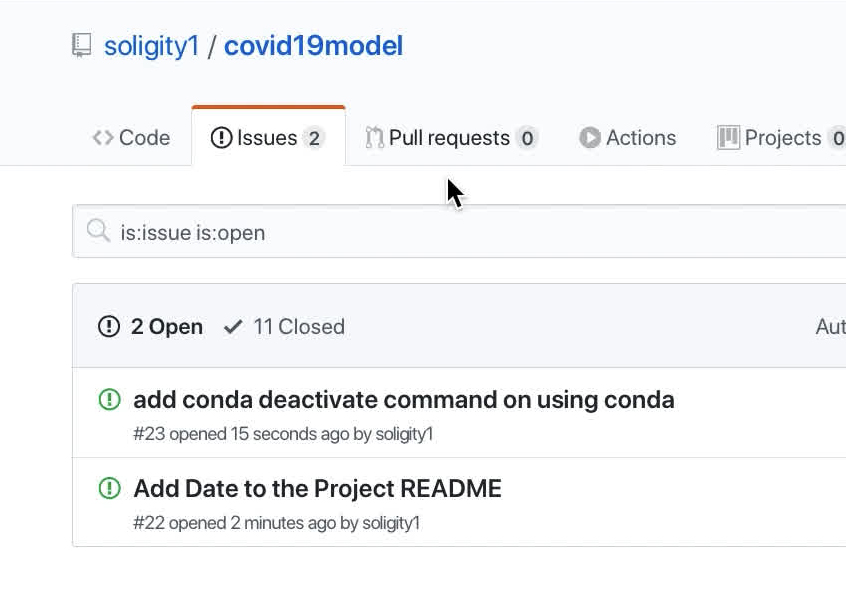
\includegraphics[height=7cm]{graphs/29. github_issues}

% 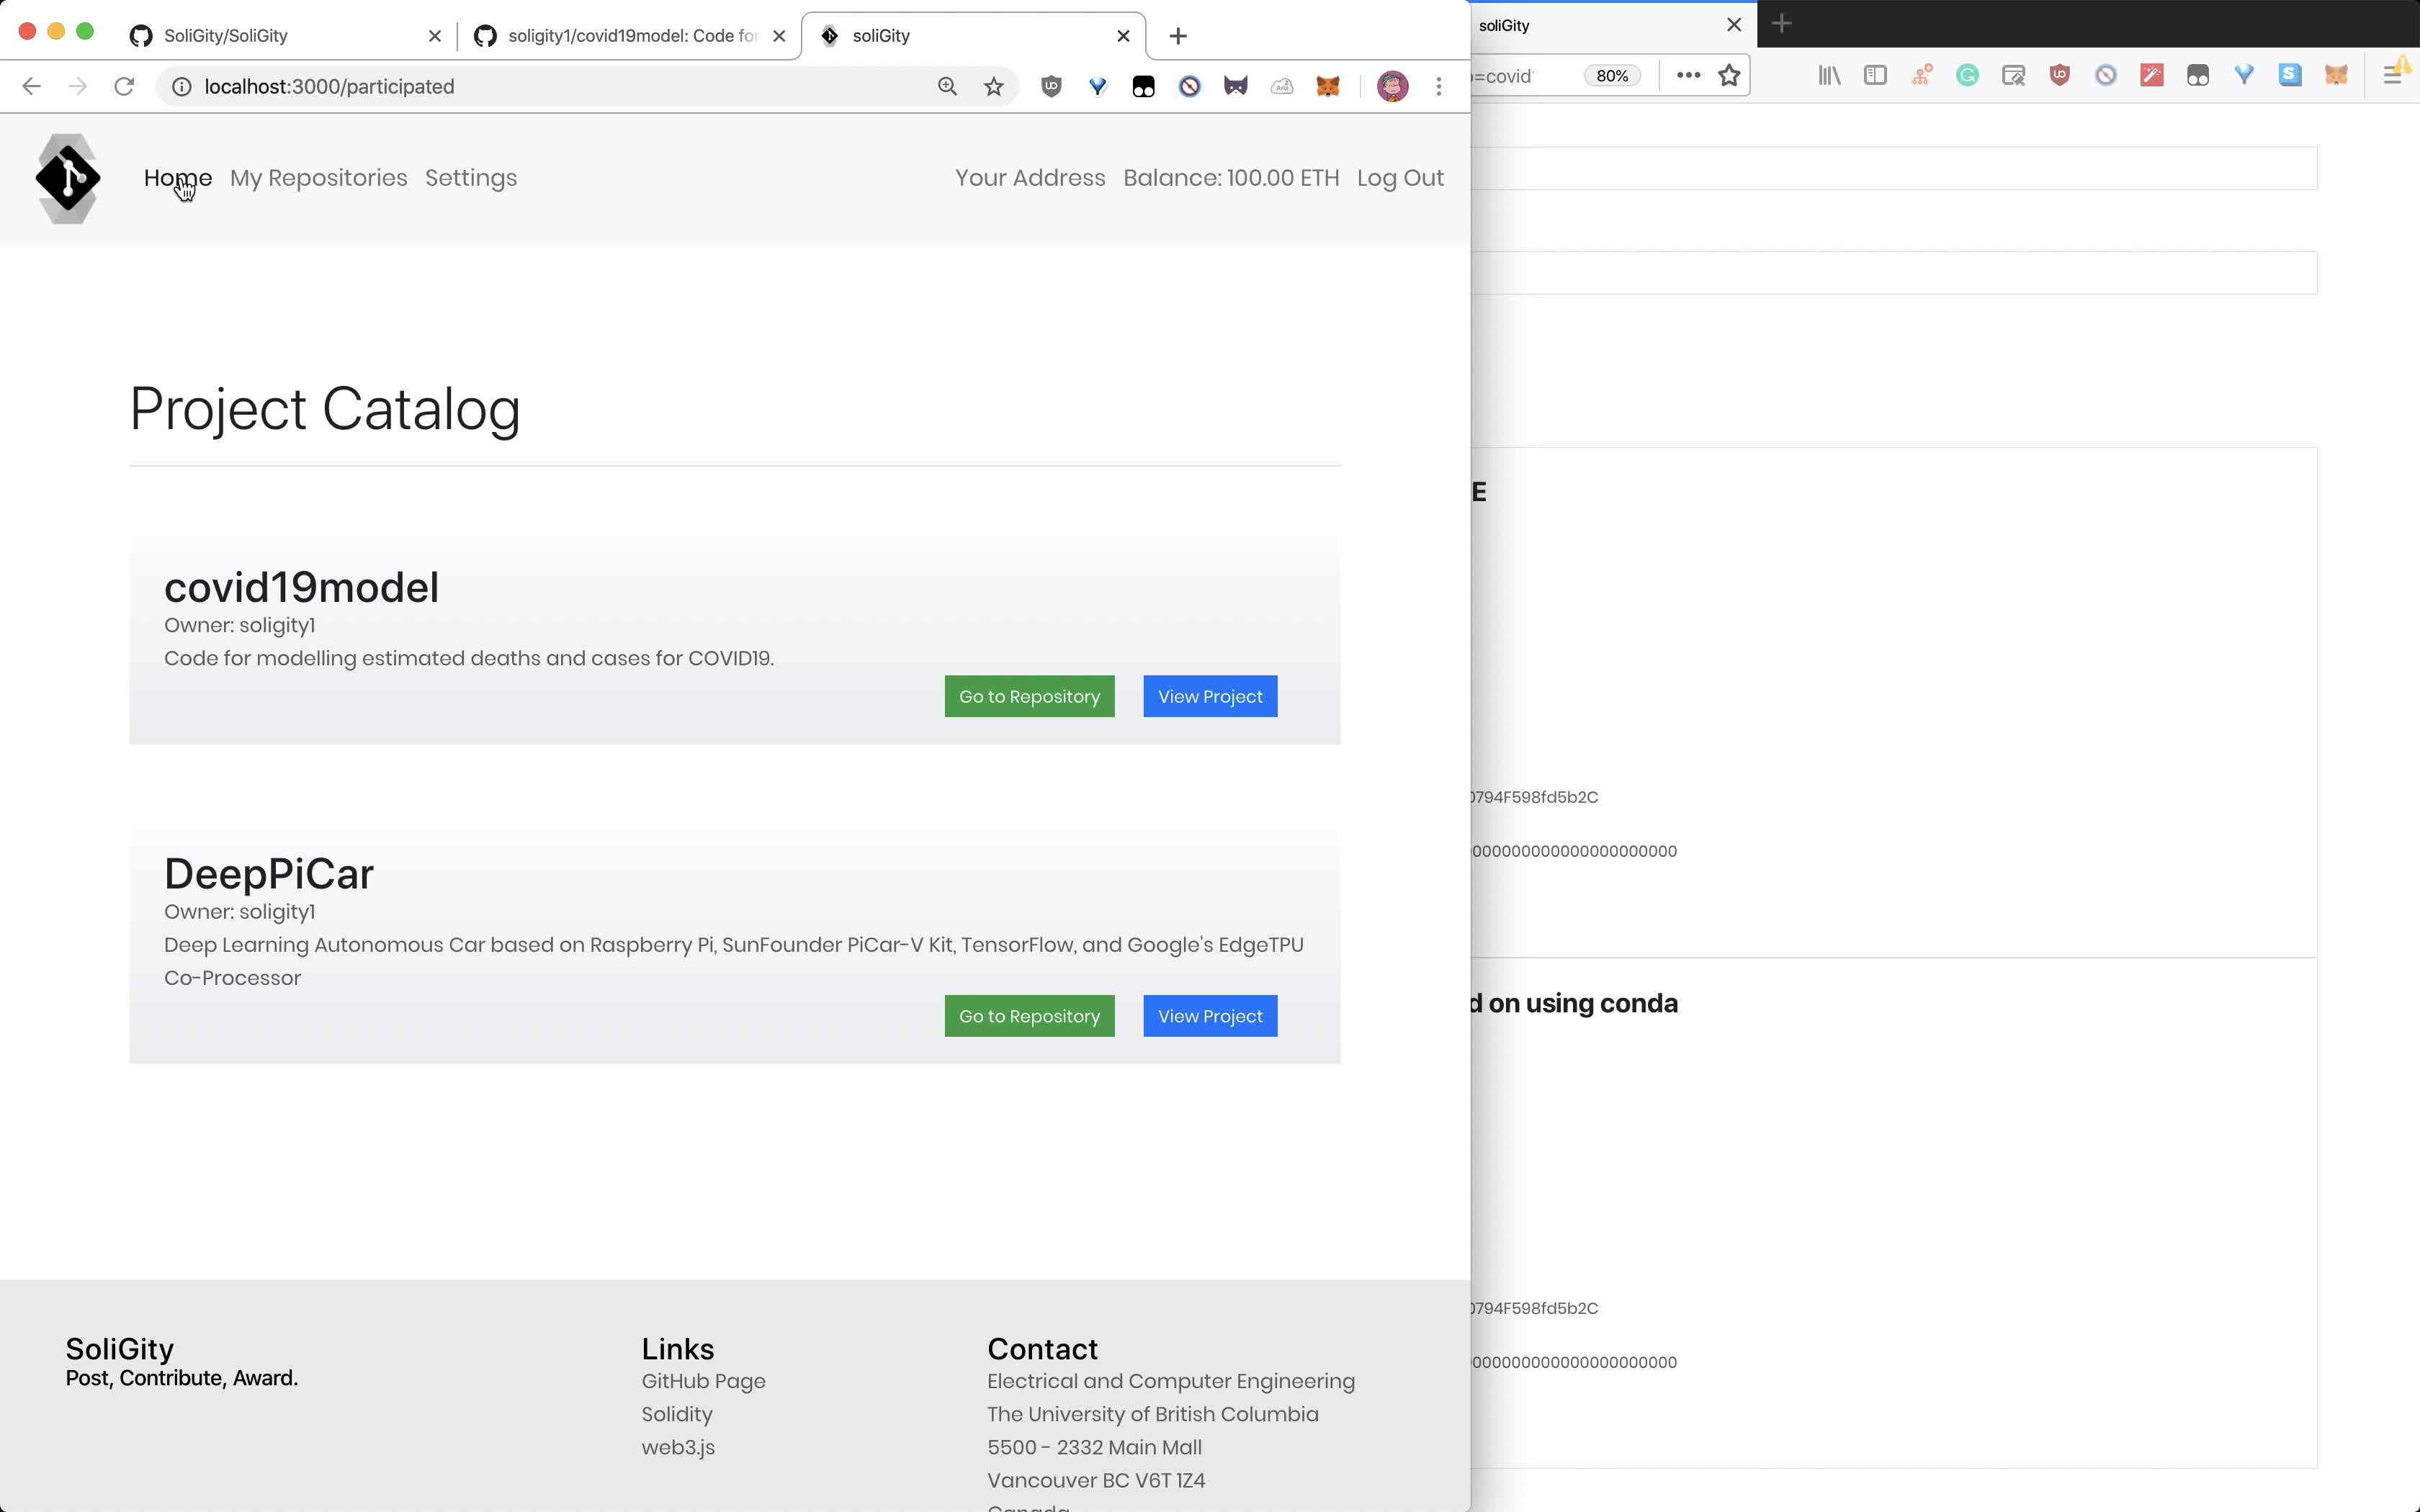
\includegraphics[height=7cm]{graphs/30. project_catalog_bob_view}

% 
\includegraphics[height=7cm]{graphs/31. bob_fork_project}

% 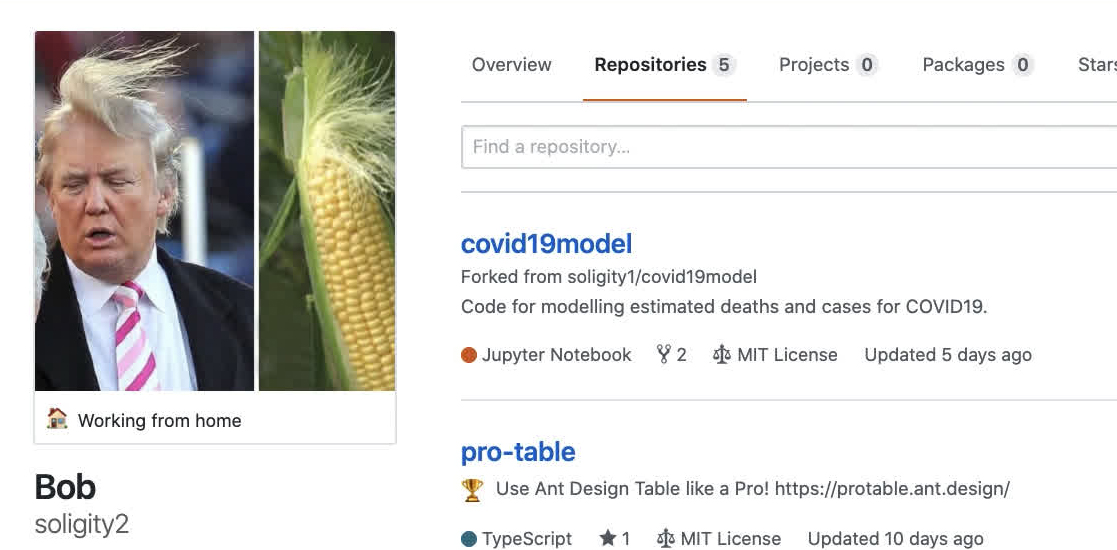
\includegraphics[height=7cm]{graphs/32. bob_forked_github}

% 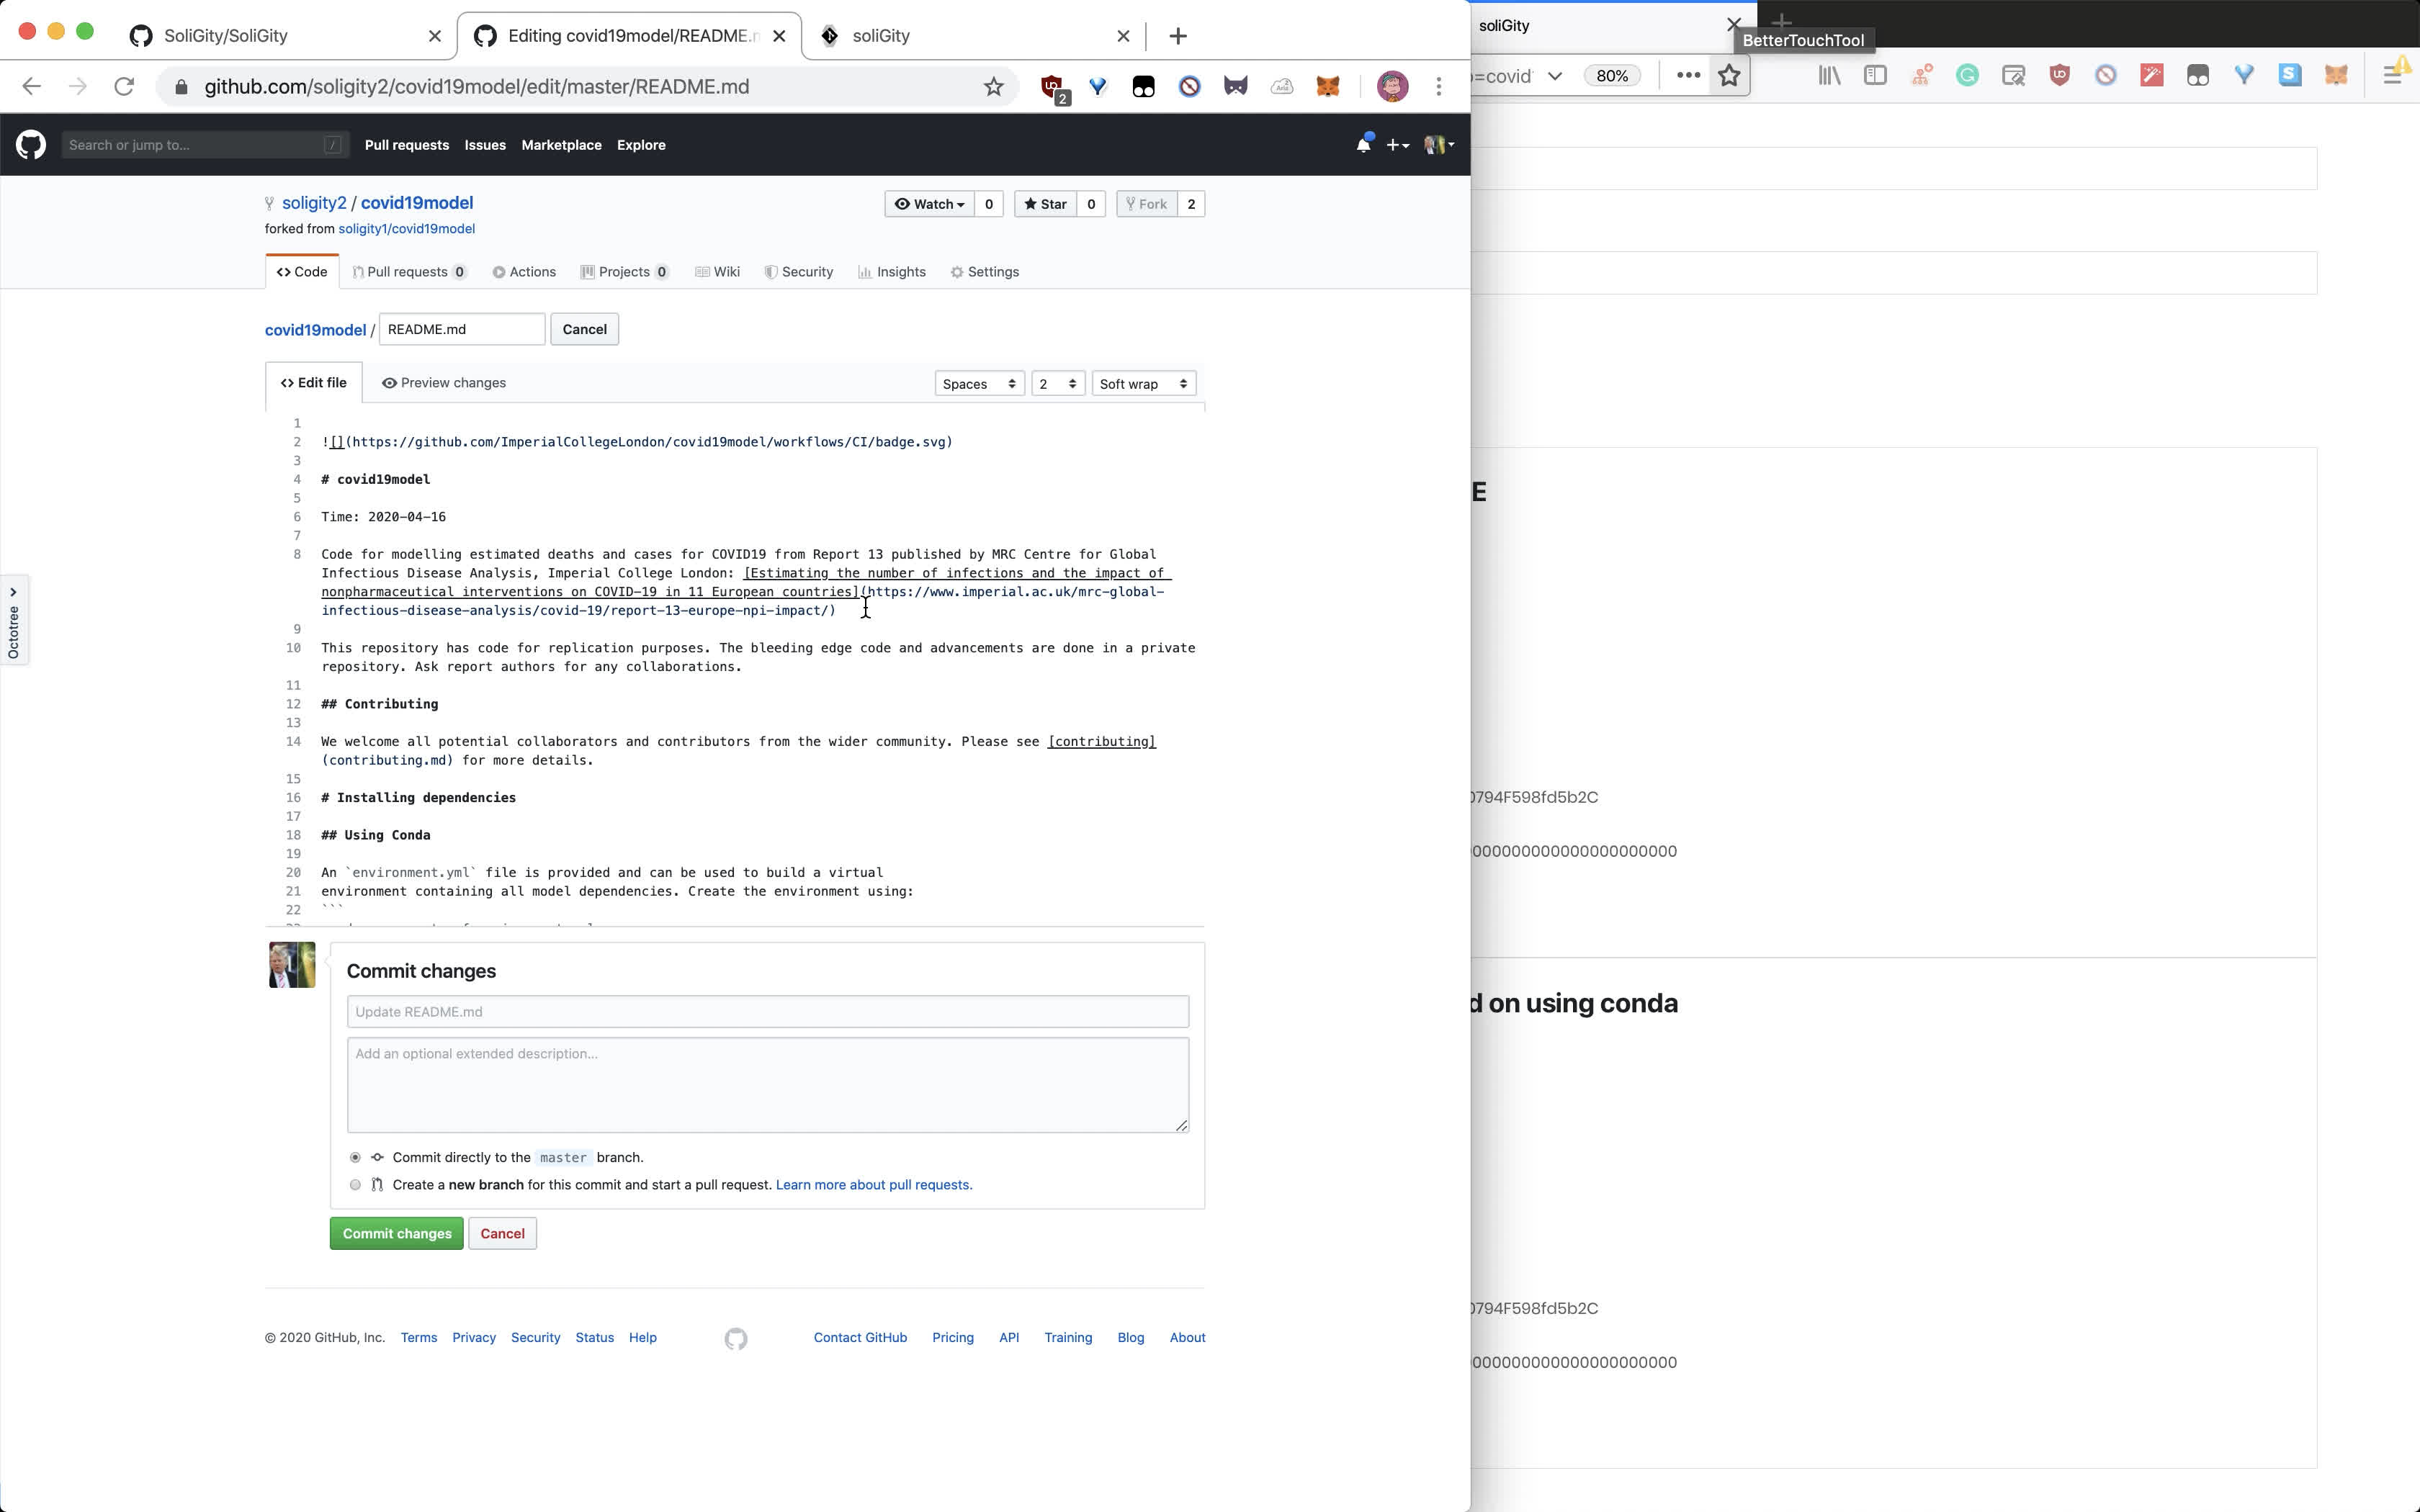
\includegraphics[height=7cm]{graphs/33. bob_make_changes}

% 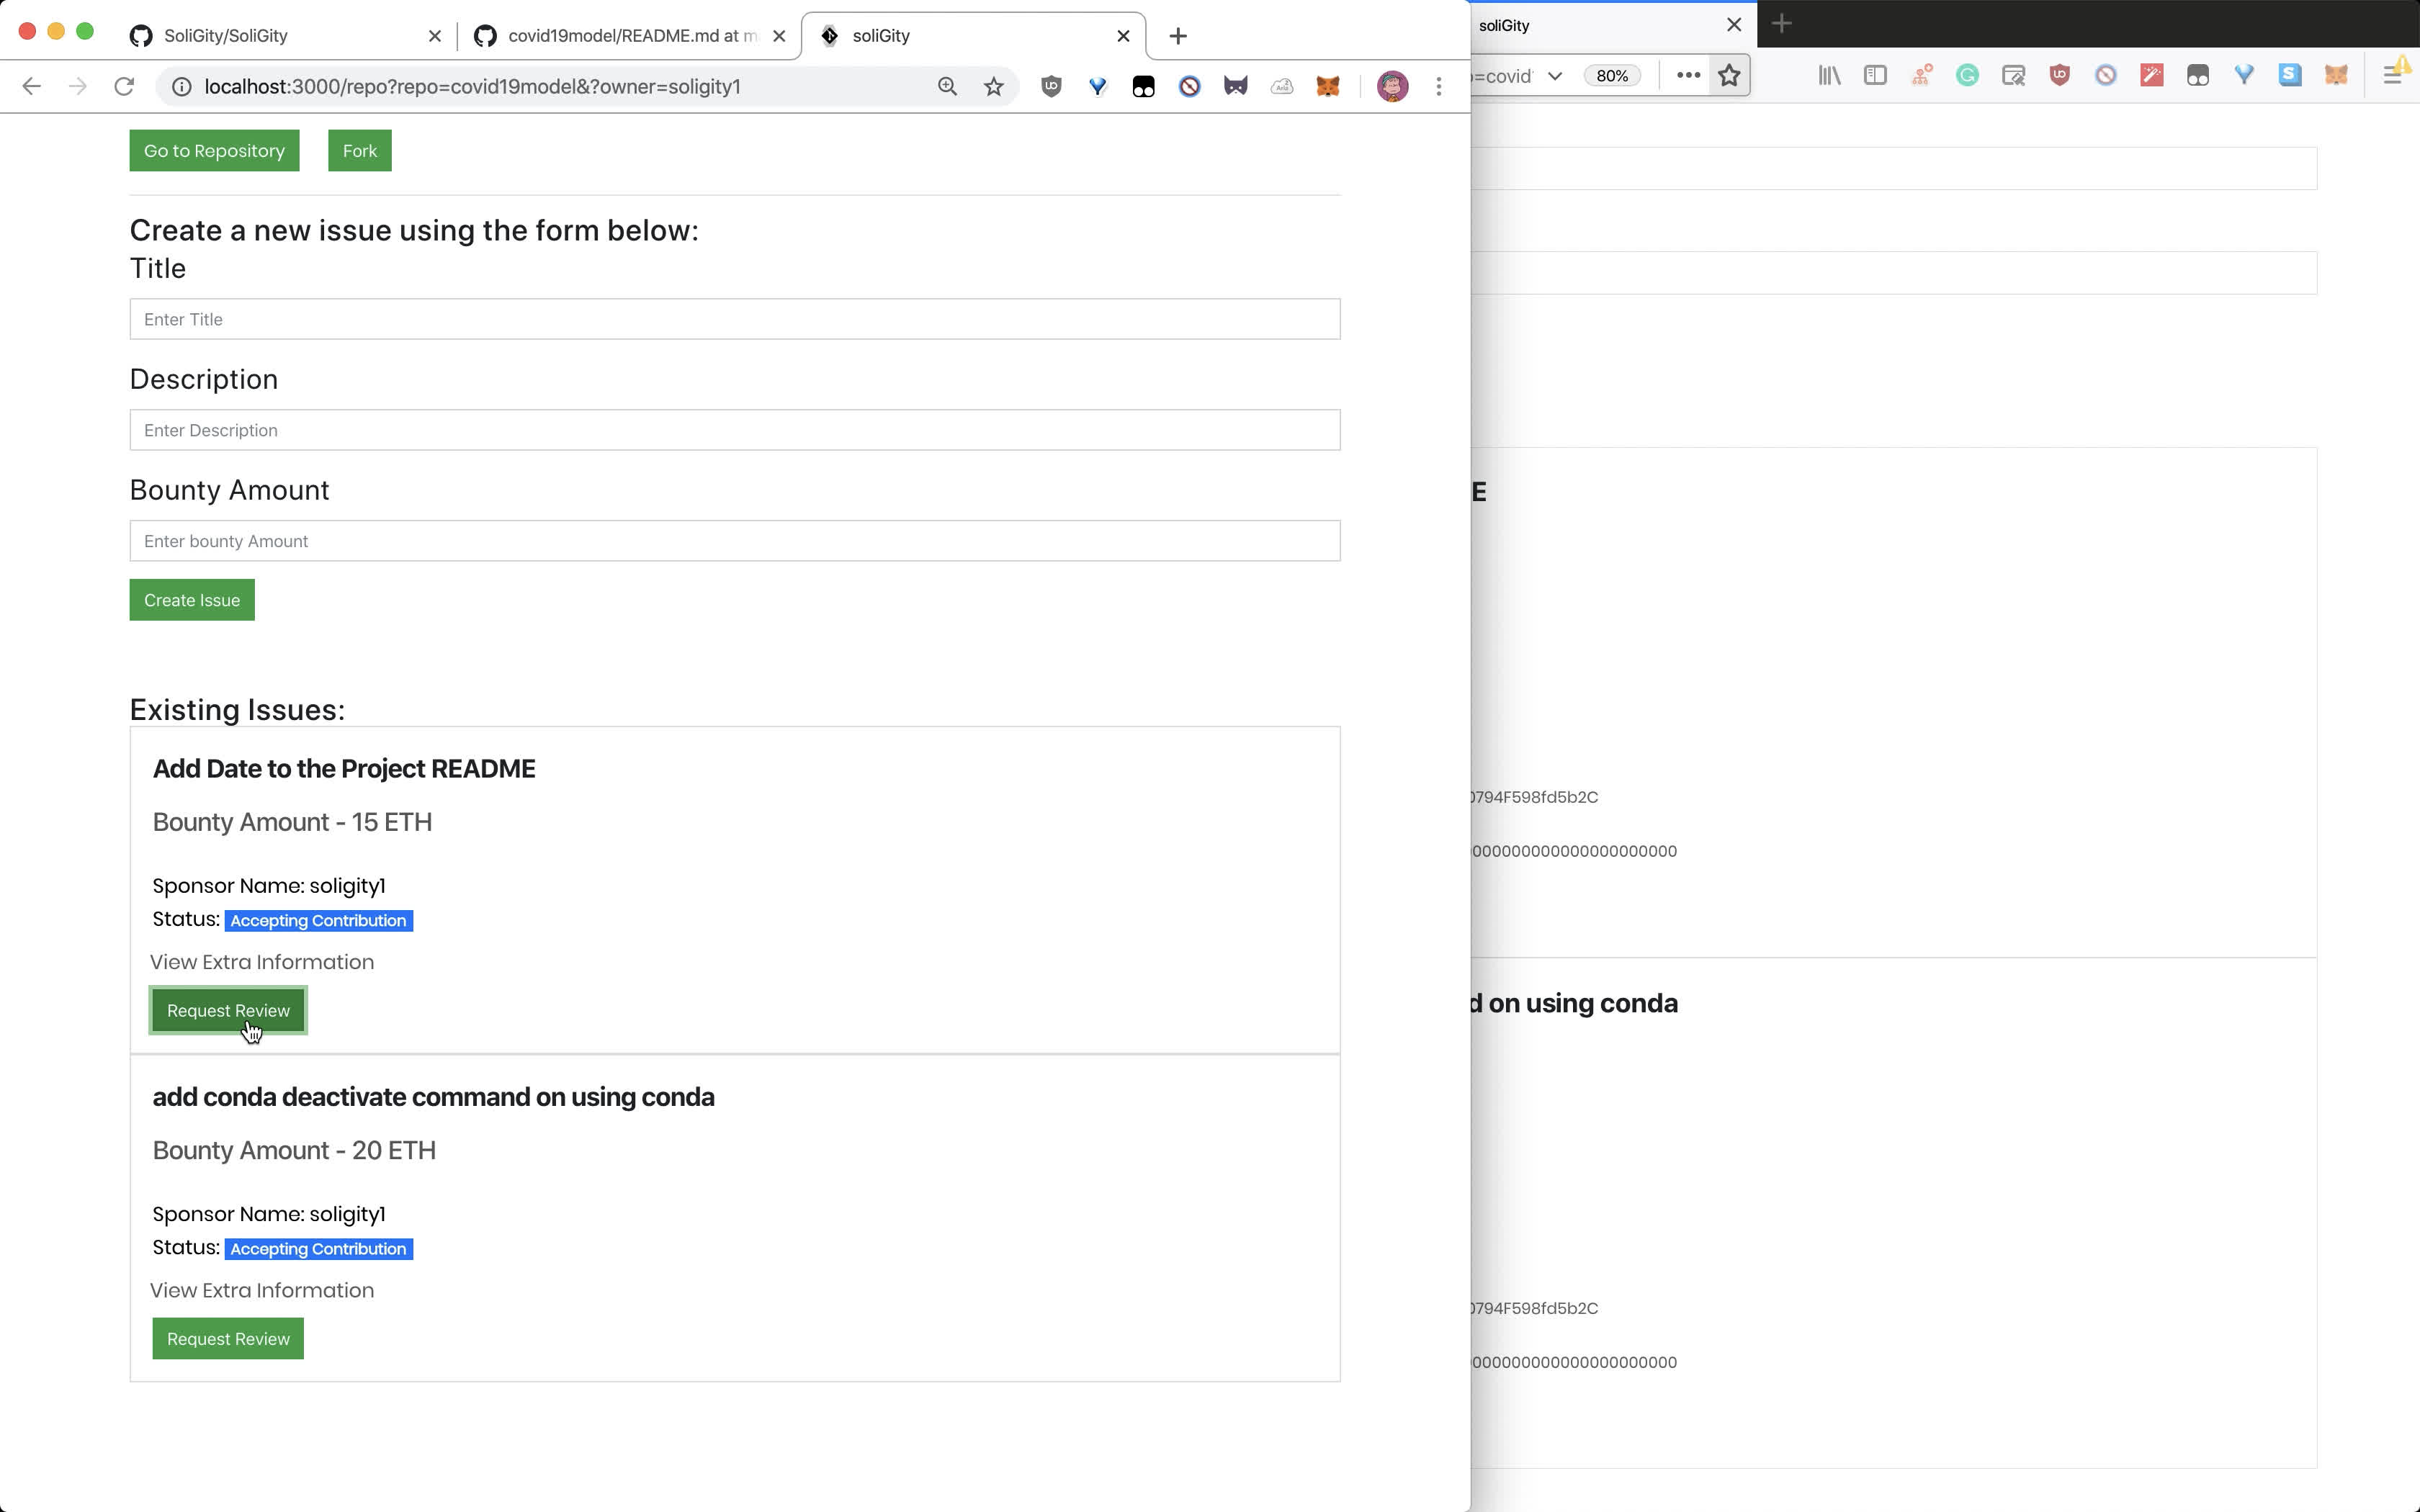
\includegraphics[height=7cm]{graphs/34. bob_review_request}

% 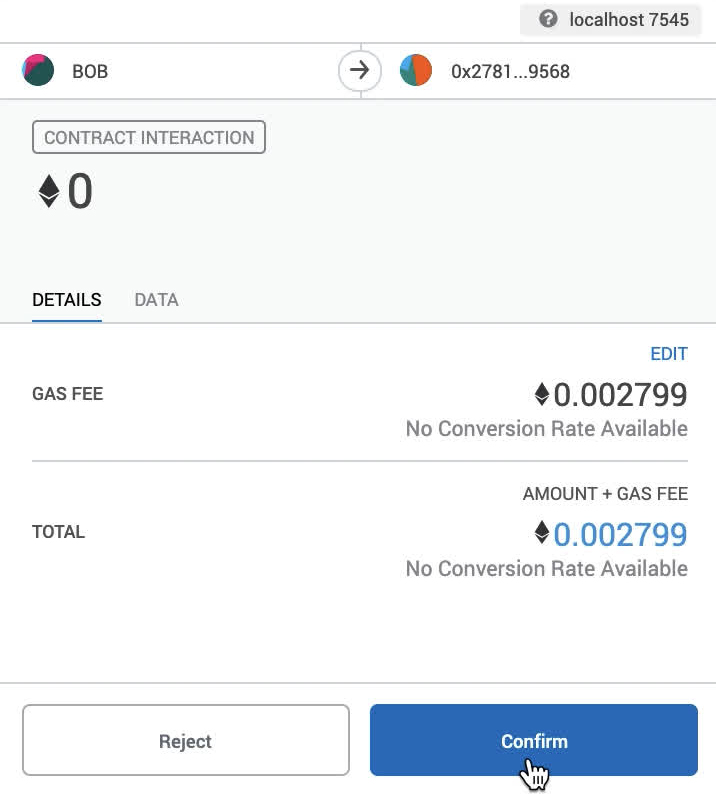
\includegraphics[height=7cm]{graphs/35. bob_review_request_metamask}

% 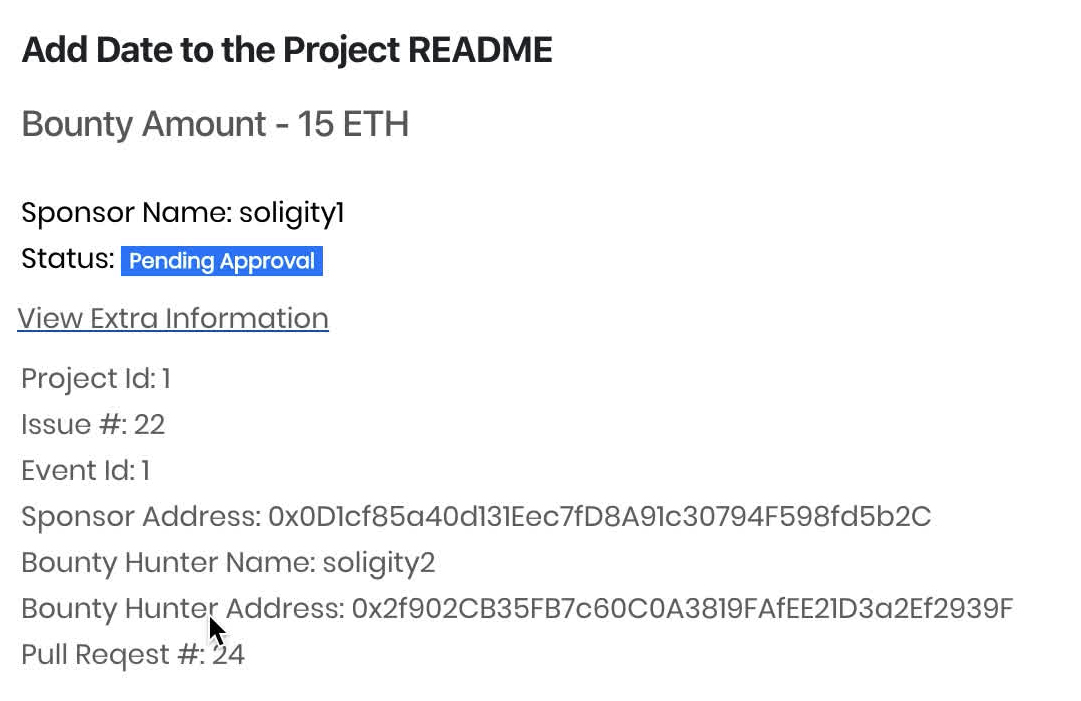
\includegraphics[height=7cm]{graphs/36. issue_info_updated}

% 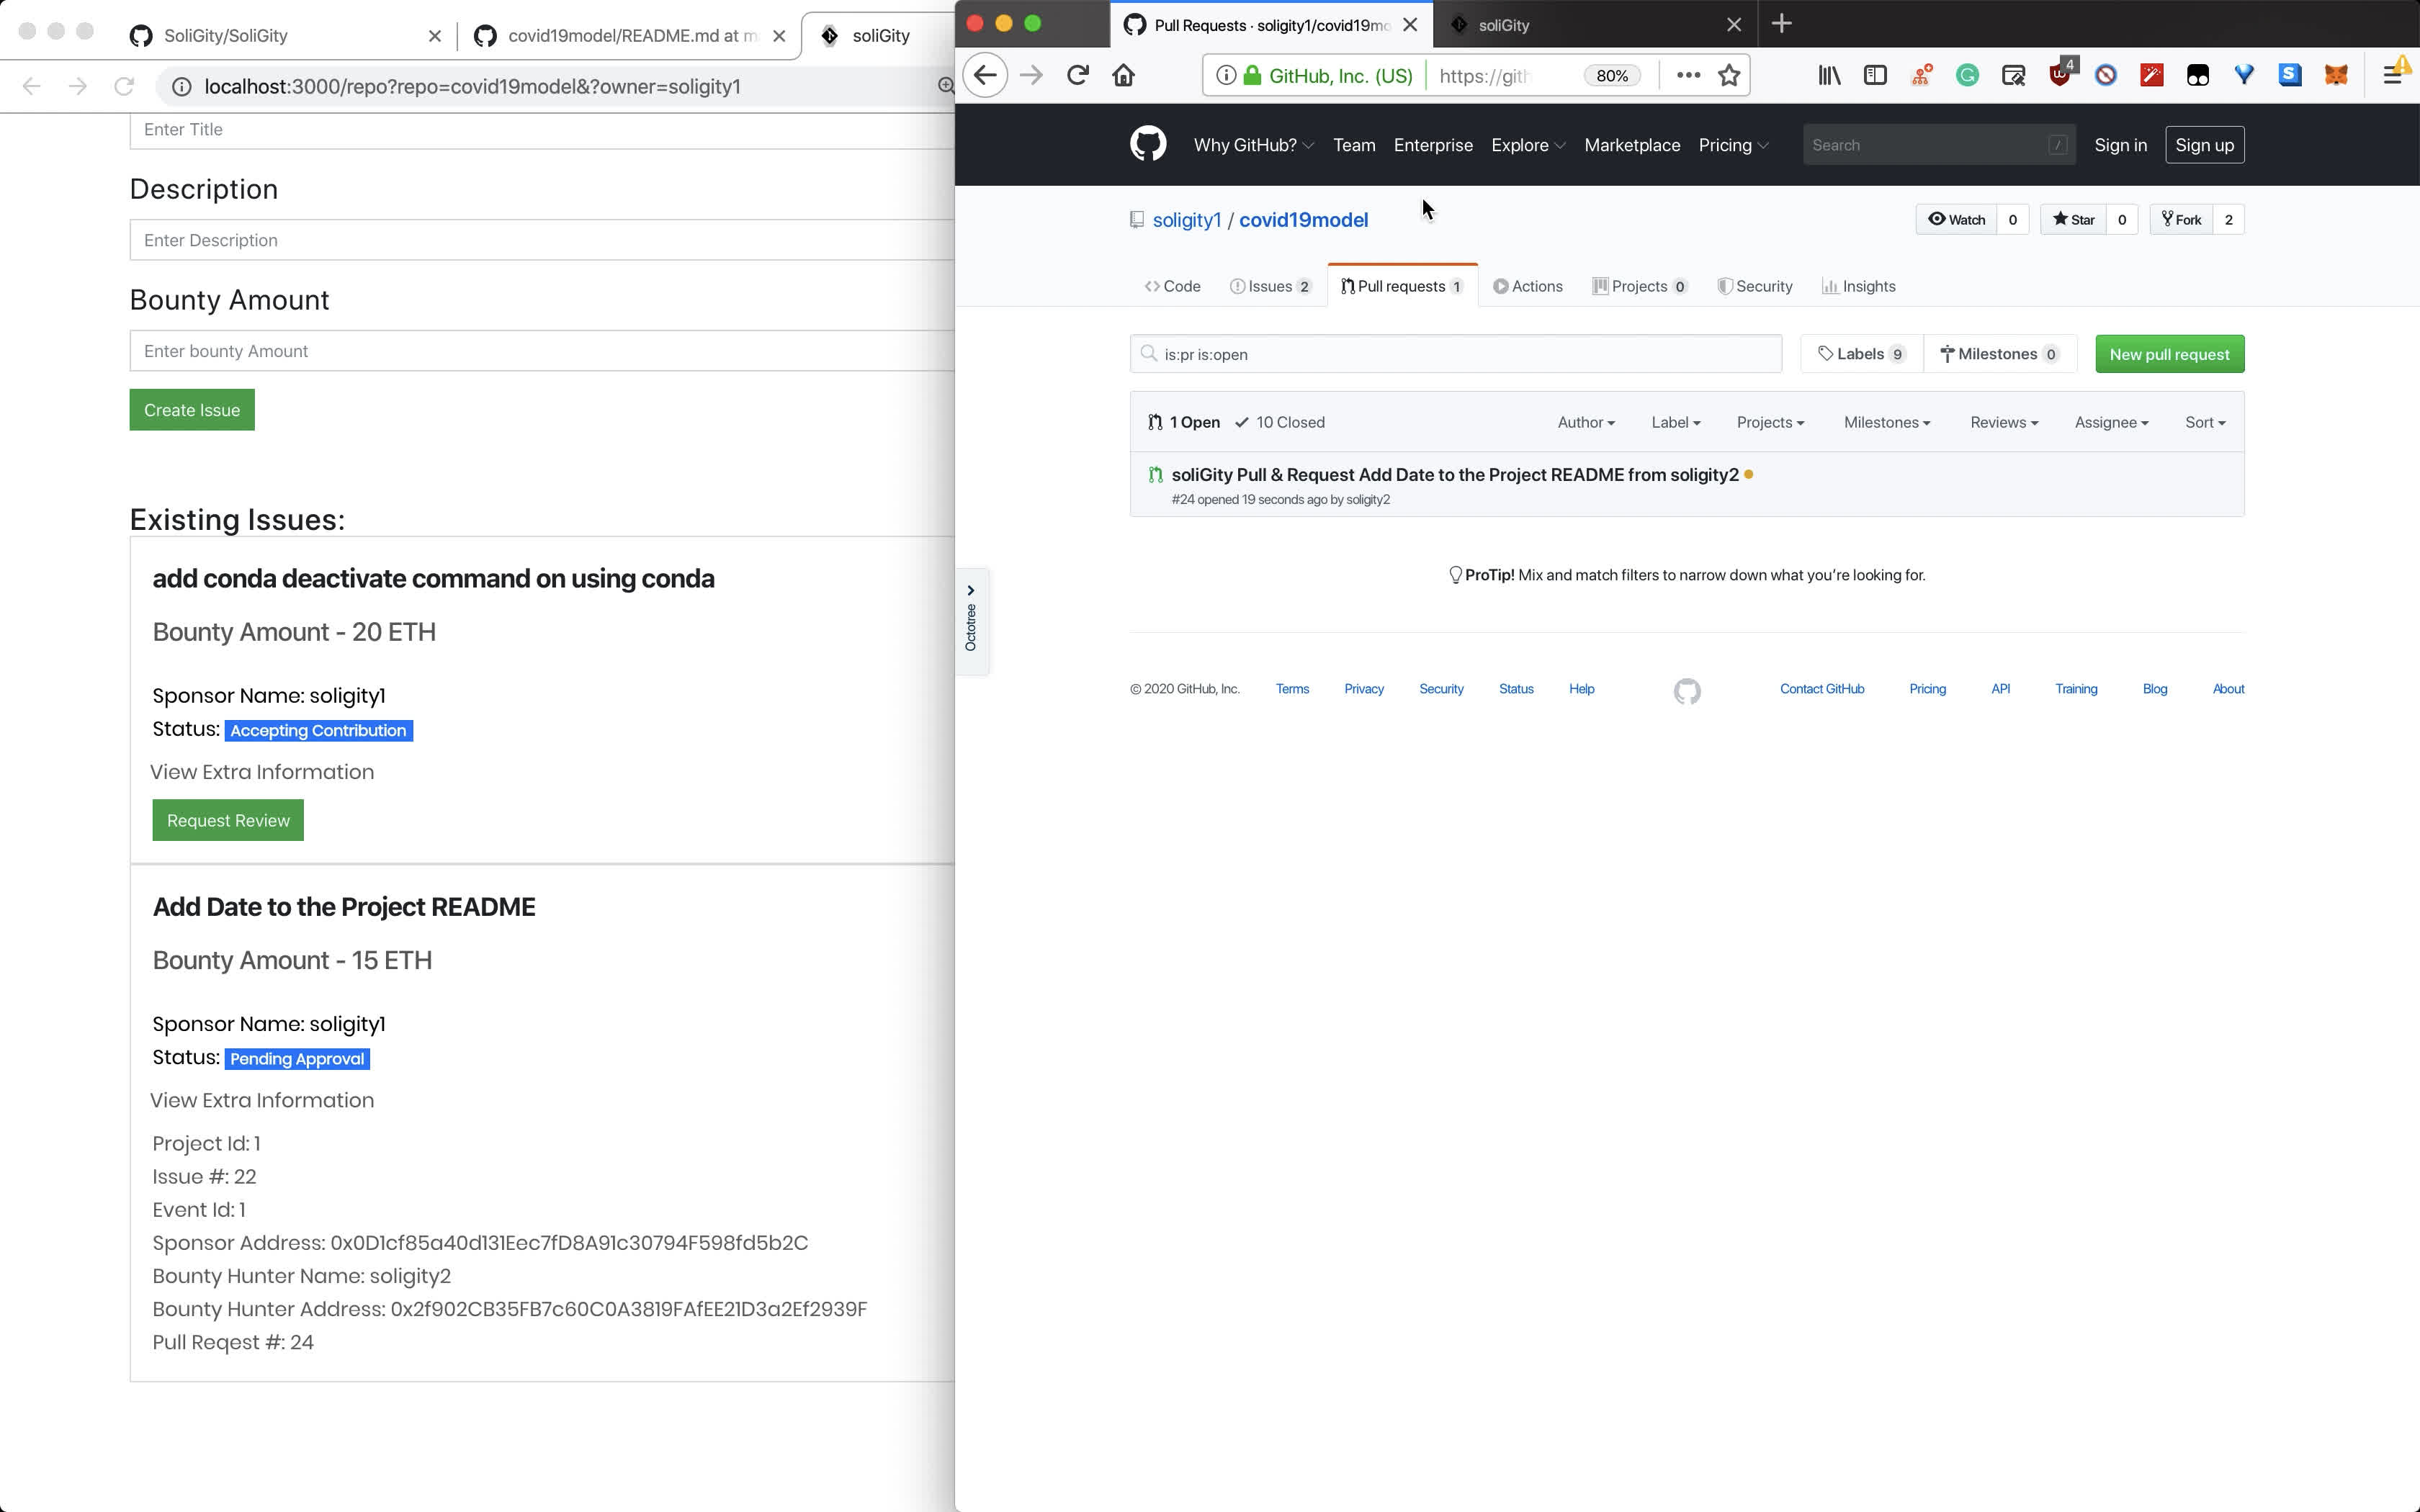
\includegraphics[height=7cm]{graphs/37. bob_pull_request_github}

% 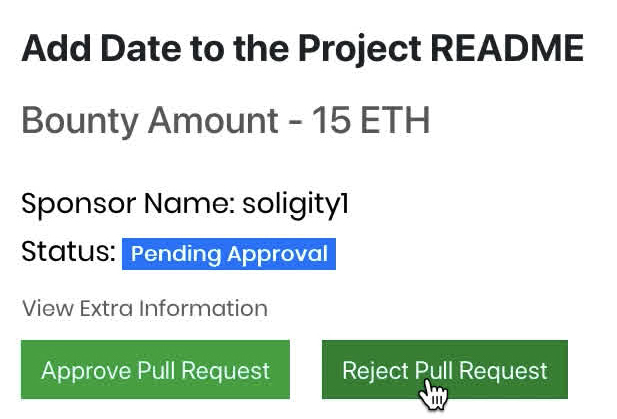
\includegraphics[height=7cm]{graphs/38. alice_reject_pull_request}

% 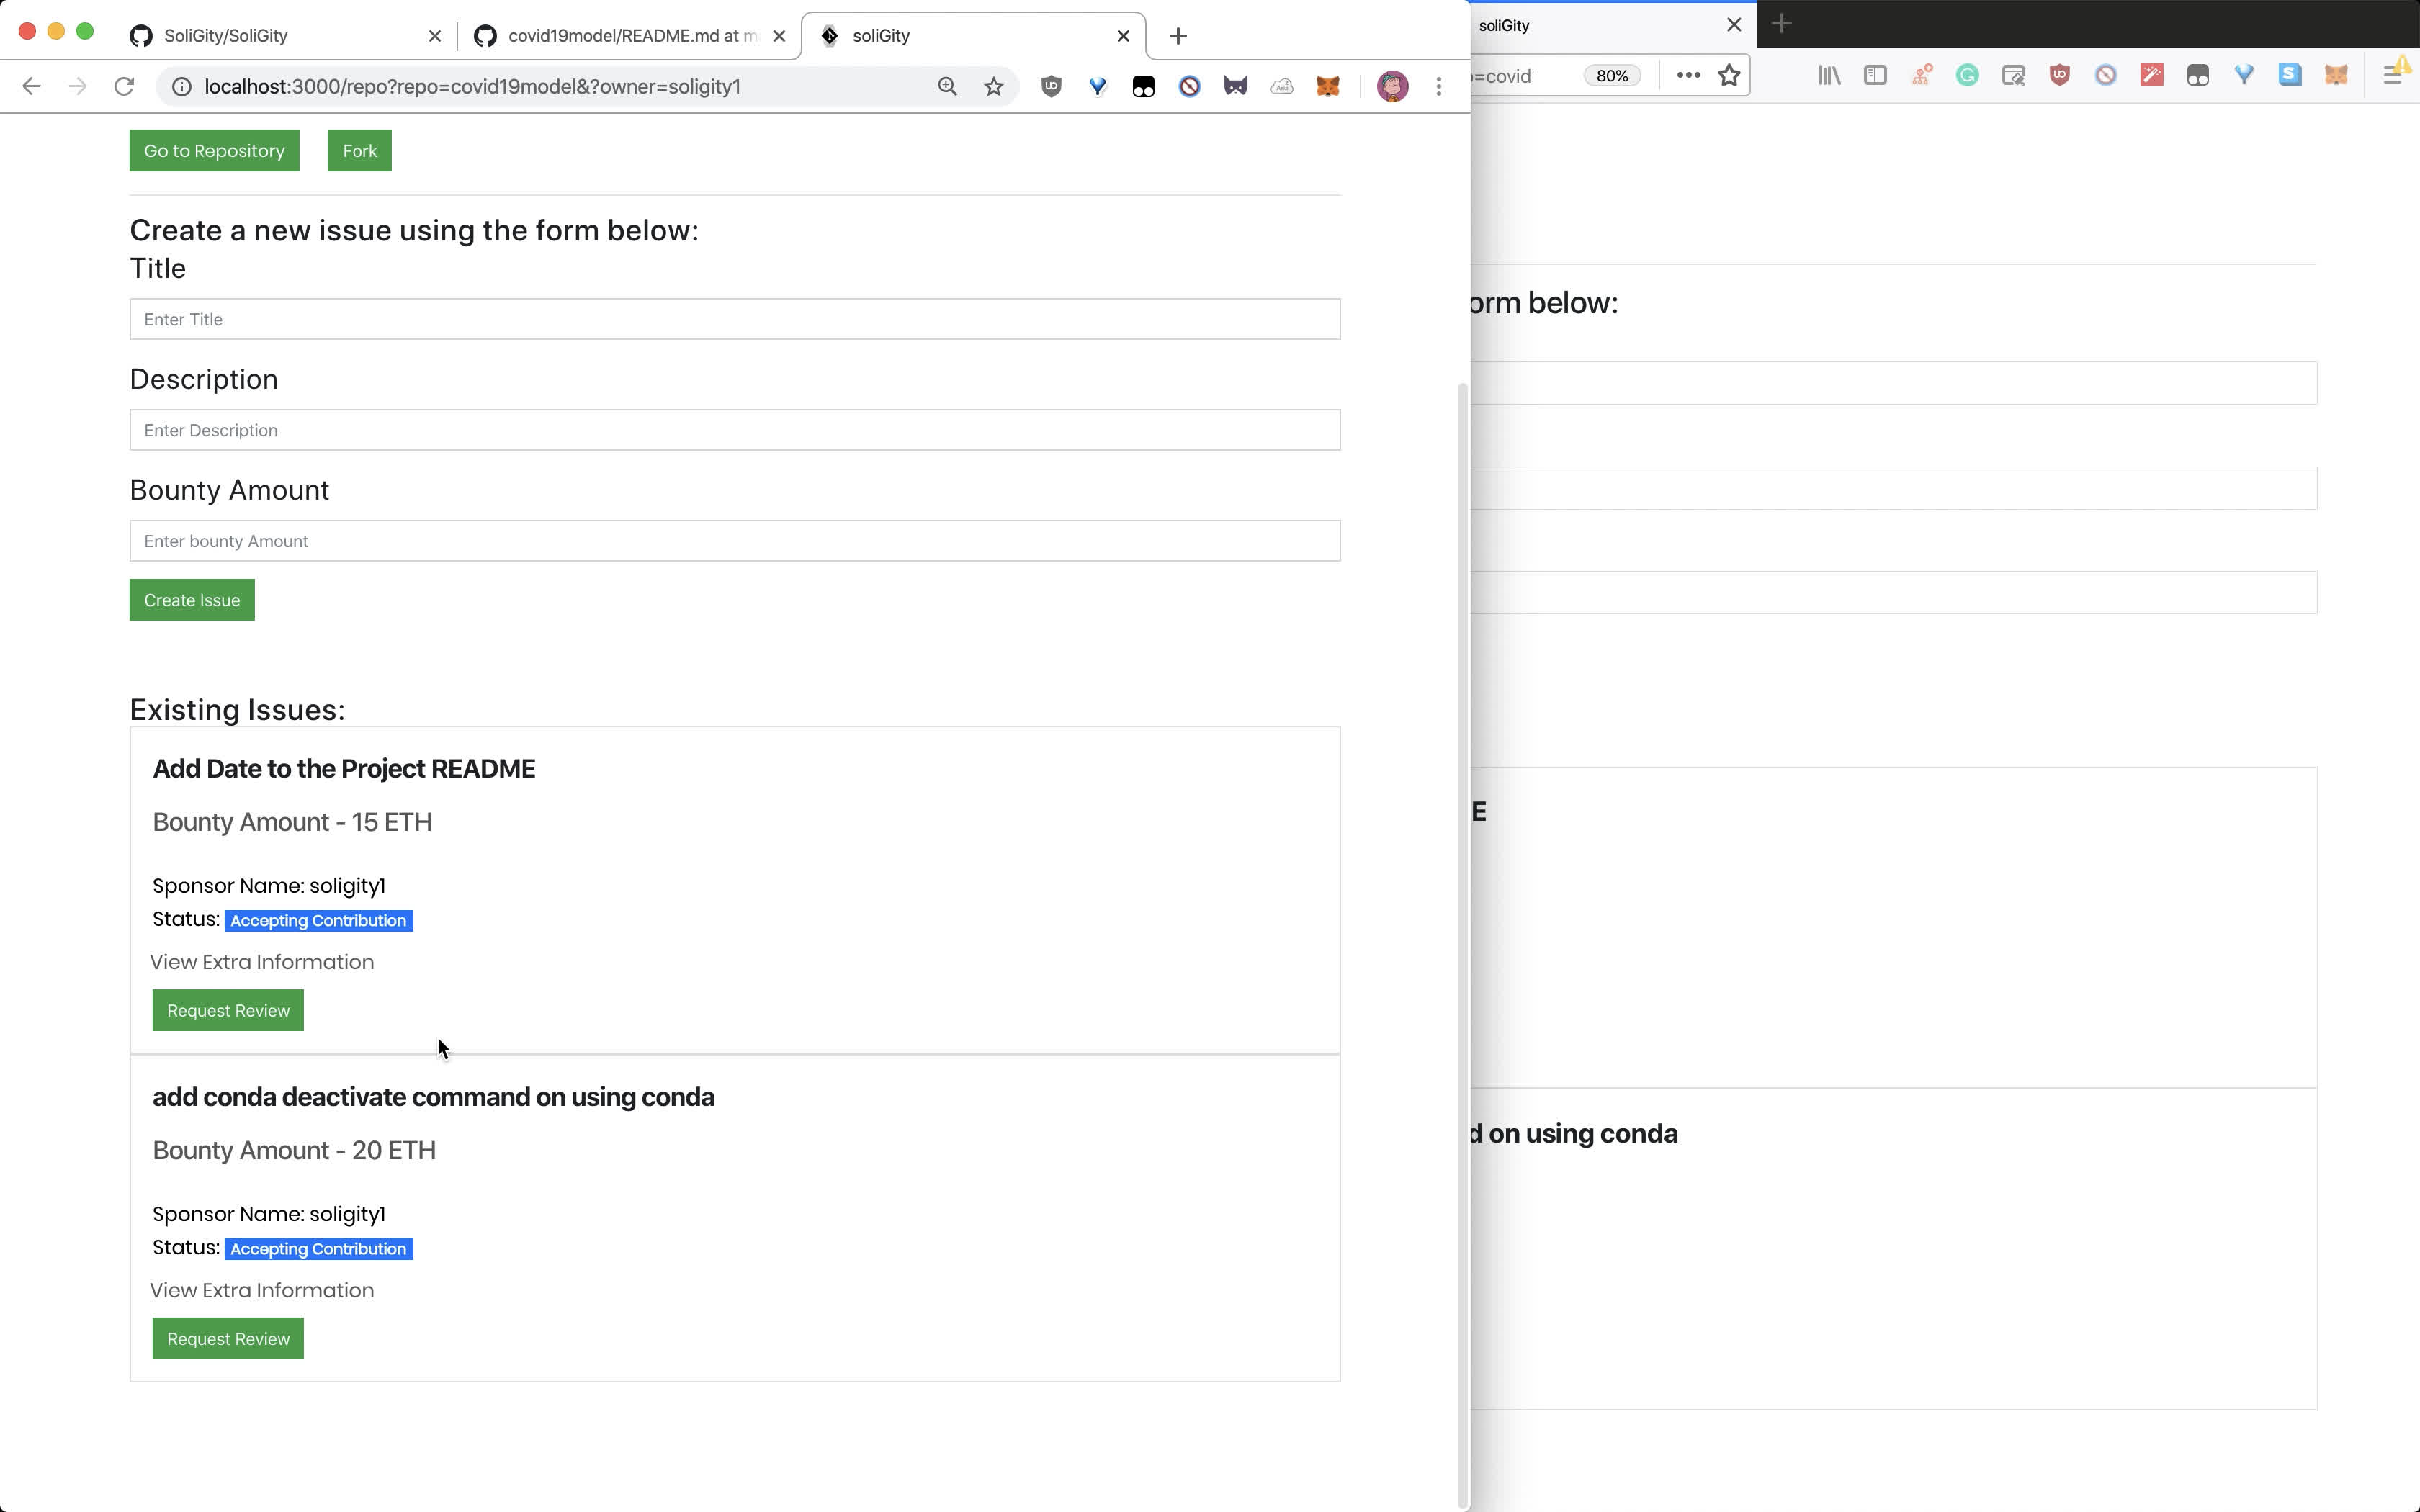
\includegraphics[height=7cm]{graphs/39. issue_info_updated}

% 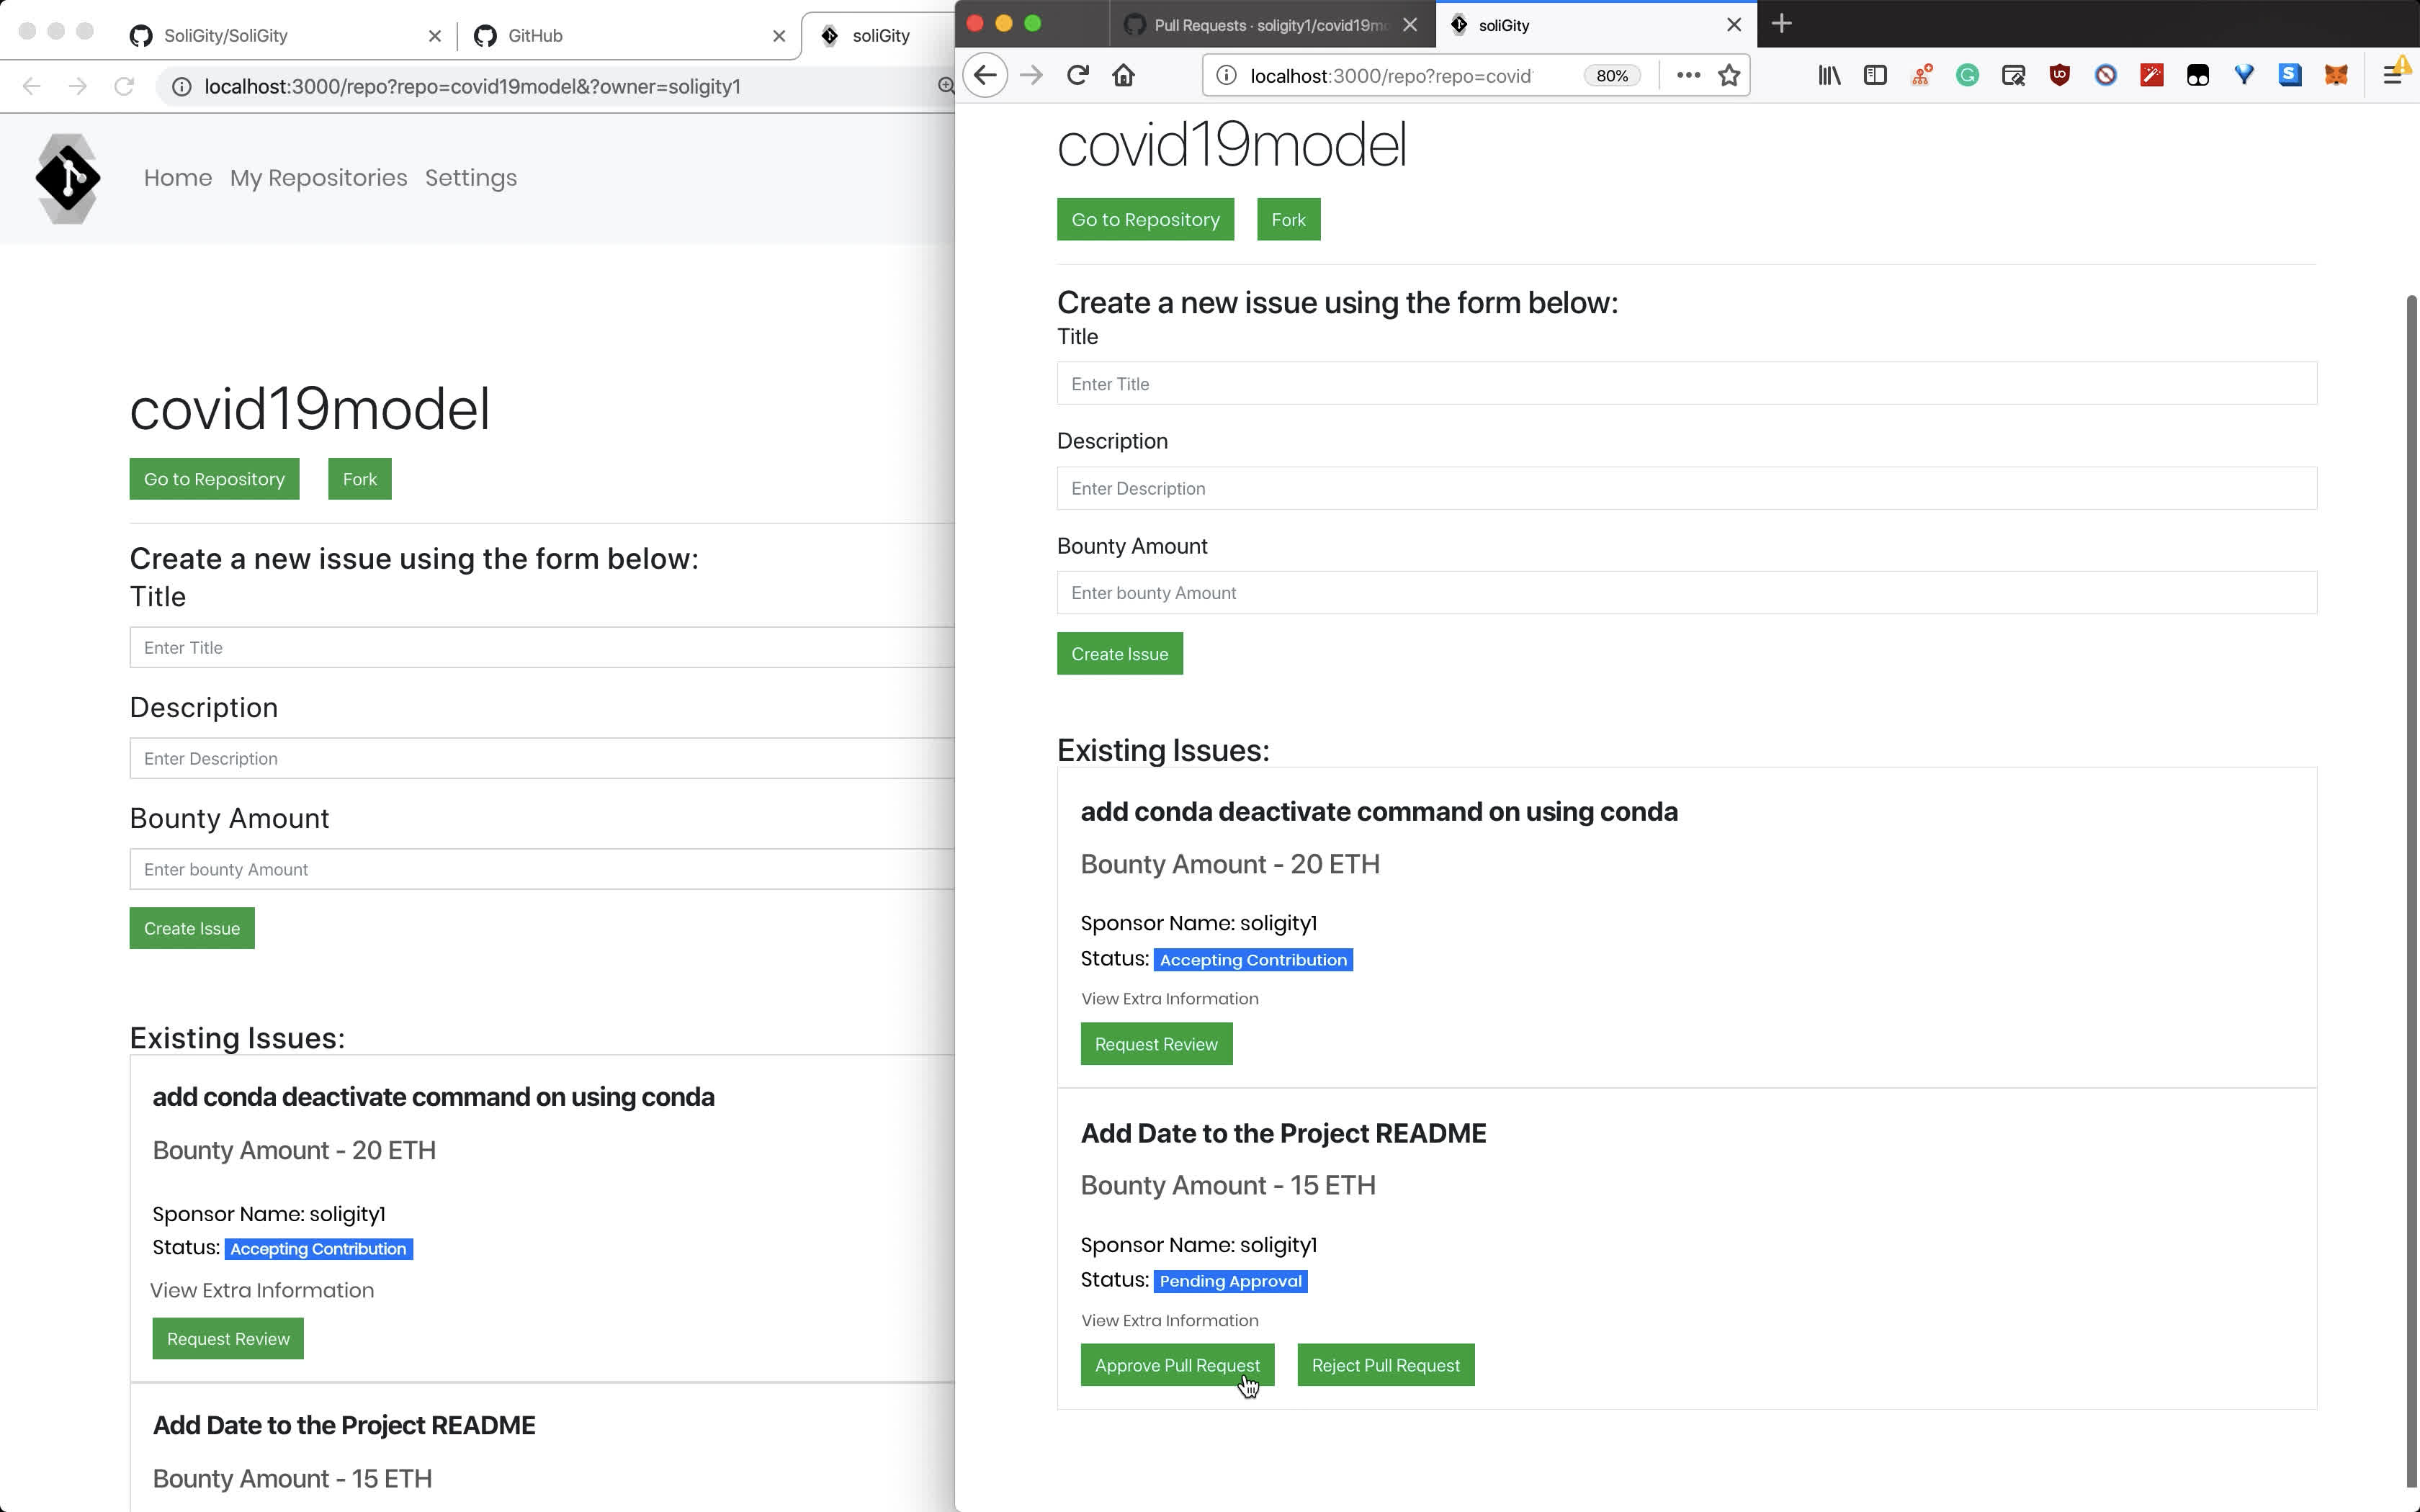
\includegraphics[height=7cm]{graphs/40. alice_approve_pull_request}

% 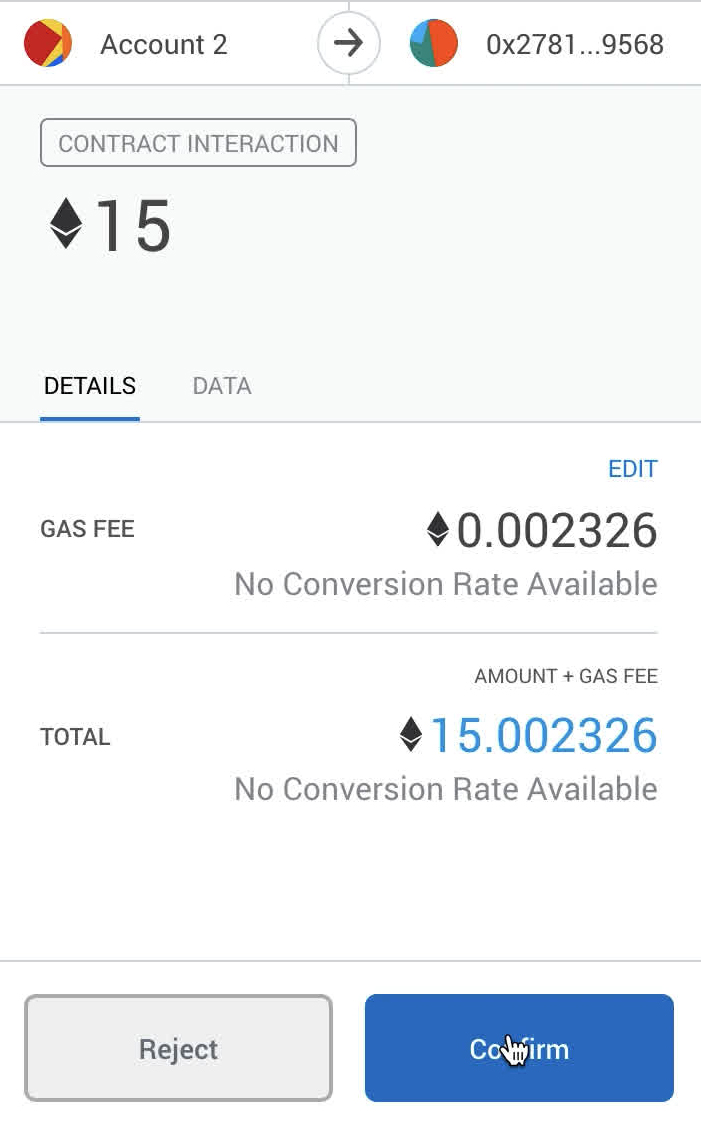
\includegraphics[height=7cm]{graphs/41. alice_metamask_confirm}

% \includegraphics[height=7cm]{graphs/42. alice_balance_updated}

% \includegraphics[height=7cm]{graphs/43. bob_balance_updated}

% \includegraphics[height=7cm]{graphs/44. pull_request_closed}

% \includegraphics[height=7cm]{graphs/45. issue_closed}



\section{Reflection}


\section{Future Work}


\section{Value Proposition}


\section{Conclusion}

\newpage


\begingroup
\raggedright

\bibliography{mybib.bib}{}
\bibliographystyle{unsrt}
\nocite{*}

\endgroup

\newpage

\begin{appendices}

	\section{Course Project Team Form}

	\begin{center}
		\textbf{Team Name: \uline{\hspace{10em}}}
	\end{center}

	\begin{table}[H]
		\centering
		\begin{tabular}{| C{2cm} | C{4cm} | C{4cm} | C{4cm} |}
			\hline
			\textbf{Index} & \textbf{Student No.} & \textbf{First Name (Printed)} & \textbf{Last Name (Printed)} \\ \hline
			1              &                      &                               &                              \\ \hline
			2              &                      &                               &                              \\ \hline
			3              &                      &                               &                              \\ \hline
			4              &                      &                               &                              \\ \hline
			5              &                      &                               &                              \\ \hline
		\end{tabular}
	\end{table}

	\begin{table}[H]
		\centering
		\begin{tabular}{| C{2cm} | C{6cm} | C{6cm} |}
			\hline
			\textbf{Index} & \textbf{Signature} & \textbf{Date} \\ \hline
			1              &                    &               \\ \hline
			2              &                    &               \\ \hline
			3              &                    &               \\ \hline
			4              &                    &               \\ \hline
			5              &                    &               \\ \hline
		\end{tabular}
	\end{table}
	\newpage

	\section{Course Project Peer-to-Peer Evaluation Form}

	\begin{center}
		\textbf{Team Name: \uline{\hspace{10em}}}
	\end{center}

	\begin{table}[H]
		\centering
		\begin{tabular}{| C{2cm} | C{4cm} | C{4cm} | C{4cm} |}
			\hline
			\textbf{Index} & \textbf{Student No.} & \textbf{First Name (Printed)} & \textbf{Last Name (Printed)} \\ \hline
			1              &                      &                               &                              \\ \hline
			2              &                      &                               &                              \\ \hline
			3              &                      &                               &                              \\ \hline
			4              &                      &                               &                              \\ \hline
			5              &                      &                               &                              \\ \hline
		\end{tabular}
	\end{table}

	\begin{table}[H]
		\centering
		\begin{tabular}{| C{2cm} | C{4cm} | C{4cm} | C{4cm} |}
			\hline
			\textbf{Index} & \textbf{Percentage} & \textbf{Signature} & \textbf{Date} \\ \hline
			1              &                     &                    &               \\ \hline
			2              &                     &                    &               \\ \hline
			3              &                     &                    &               \\ \hline
			4              &                     &                    &               \\ \hline
			5              &                     &                    &               \\ \hline
		\end{tabular}
	\end{table}
	\newpage

\end{appendices}

\end{document}